\documentclass{article}

\usepackage{arxiv}

\usepackage[utf8]{inputenc} % allow utf-8 input
\usepackage[T1]{fontenc}    % use 8-bit T1 fonts
\usepackage{lmodern}        % https://github.com/rstudio/rticles/issues/343
\usepackage{hyperref}       % hyperlinks
\usepackage{url}            % simple URL typesetting
\usepackage{booktabs}       % professional-quality tables
\usepackage{amsfonts}       % blackboard math symbols
\usepackage{nicefrac}       % compact symbols for 1/2, etc.
\usepackage{microtype}      % microtypography
\usepackage{lipsum}
\usepackage{graphicx}

\title{Avaliação de imóveis a partir de dados de oferta}

\author{
    Luiz Fernando Palin Droubi
   \\
    SPU/SC \\
    Secretaria de Coordenação e Governança do Patrimônio da União \\
  Florianópolis, SC \\
  \texttt{\href{mailto:lfpdroubi@gmail.com}{\nolinkurl{lfpdroubi@gmail.com}}} \\
  }

\usepackage{color}
\usepackage{fancyvrb}
\newcommand{\VerbBar}{|}
\newcommand{\VERB}{\Verb[commandchars=\\\{\}]}
\DefineVerbatimEnvironment{Highlighting}{Verbatim}{commandchars=\\\{\}}
% Add ',fontsize=\small' for more characters per line
\usepackage{framed}
\definecolor{shadecolor}{RGB}{248,248,248}
\newenvironment{Shaded}{\begin{snugshade}}{\end{snugshade}}
\newcommand{\AlertTok}[1]{\textcolor[rgb]{0.94,0.16,0.16}{#1}}
\newcommand{\AnnotationTok}[1]{\textcolor[rgb]{0.56,0.35,0.01}{\textbf{\textit{#1}}}}
\newcommand{\AttributeTok}[1]{\textcolor[rgb]{0.77,0.63,0.00}{#1}}
\newcommand{\BaseNTok}[1]{\textcolor[rgb]{0.00,0.00,0.81}{#1}}
\newcommand{\BuiltInTok}[1]{#1}
\newcommand{\CharTok}[1]{\textcolor[rgb]{0.31,0.60,0.02}{#1}}
\newcommand{\CommentTok}[1]{\textcolor[rgb]{0.56,0.35,0.01}{\textit{#1}}}
\newcommand{\CommentVarTok}[1]{\textcolor[rgb]{0.56,0.35,0.01}{\textbf{\textit{#1}}}}
\newcommand{\ConstantTok}[1]{\textcolor[rgb]{0.00,0.00,0.00}{#1}}
\newcommand{\ControlFlowTok}[1]{\textcolor[rgb]{0.13,0.29,0.53}{\textbf{#1}}}
\newcommand{\DataTypeTok}[1]{\textcolor[rgb]{0.13,0.29,0.53}{#1}}
\newcommand{\DecValTok}[1]{\textcolor[rgb]{0.00,0.00,0.81}{#1}}
\newcommand{\DocumentationTok}[1]{\textcolor[rgb]{0.56,0.35,0.01}{\textbf{\textit{#1}}}}
\newcommand{\ErrorTok}[1]{\textcolor[rgb]{0.64,0.00,0.00}{\textbf{#1}}}
\newcommand{\ExtensionTok}[1]{#1}
\newcommand{\FloatTok}[1]{\textcolor[rgb]{0.00,0.00,0.81}{#1}}
\newcommand{\FunctionTok}[1]{\textcolor[rgb]{0.00,0.00,0.00}{#1}}
\newcommand{\ImportTok}[1]{#1}
\newcommand{\InformationTok}[1]{\textcolor[rgb]{0.56,0.35,0.01}{\textbf{\textit{#1}}}}
\newcommand{\KeywordTok}[1]{\textcolor[rgb]{0.13,0.29,0.53}{\textbf{#1}}}
\newcommand{\NormalTok}[1]{#1}
\newcommand{\OperatorTok}[1]{\textcolor[rgb]{0.81,0.36,0.00}{\textbf{#1}}}
\newcommand{\OtherTok}[1]{\textcolor[rgb]{0.56,0.35,0.01}{#1}}
\newcommand{\PreprocessorTok}[1]{\textcolor[rgb]{0.56,0.35,0.01}{\textit{#1}}}
\newcommand{\RegionMarkerTok}[1]{#1}
\newcommand{\SpecialCharTok}[1]{\textcolor[rgb]{0.00,0.00,0.00}{#1}}
\newcommand{\SpecialStringTok}[1]{\textcolor[rgb]{0.31,0.60,0.02}{#1}}
\newcommand{\StringTok}[1]{\textcolor[rgb]{0.31,0.60,0.02}{#1}}
\newcommand{\VariableTok}[1]{\textcolor[rgb]{0.00,0.00,0.00}{#1}}
\newcommand{\VerbatimStringTok}[1]{\textcolor[rgb]{0.31,0.60,0.02}{#1}}
\newcommand{\WarningTok}[1]{\textcolor[rgb]{0.56,0.35,0.01}{\textbf{\textit{#1}}}}

% Pandoc citation processing

\usepackage{amsmath}
\usepackage{float}
\usepackage[brazil]{babel}


\begin{document}
\maketitle

\def\tightlist{}


\begin{abstract}
Um dos grandes problemas práticos da Engenharia de Avaliações no Brasil
é a falta de dados de mercado envolvendo transações de imóveis para
elaboração de avaliações com o Método Comparativo de Dados de Mercado. É
usual, portanto, a utilização de dados de oferta para a confecção de
modelos estatísticos, visando utilizá-la como parâmetro para a aferição
do valor de venda. Este trabalho pretende demonstrar diversas formas
para o tratamento destes dados de oferta, buscando um conjunto de
procedimentos que propriciem a obtenção de resultados consistentes,
qualquer quer seja o método aplicado.
\end{abstract}

\keywords{
    Fator Oferta
   \and
    Campo de Arbítrio
   \and
    Intervalos admissíveis
  }

\hypertarget{introduuxe7uxe3o}{%
\section{Introdução}\label{introduuxe7uxe3o}}

De acordo com Mooya (\protect\hyperlink{ref-mooya2009}{2009}), \ldots{}

Chinloy (\protect\hyperlink{ref-chinloy}{1980}) parece ter sido o
primeiro trabalho a abordar o fator oferta de maneira científica.

Posteriormente, Horowitz
(\protect\hyperlink{ref-horowitz}{1992})\ldots{}

Haurin et al.~(\protect\hyperlink{ref-haurin}{2013}) mostram que, em
períodos de \emph{boom} no mercado imobiliário, os preços de venda podem
superar os preços listados.

\hypertarget{revisuxe3o-bibliogruxe1fica}{%
\section{Revisão Bibliográfica}\label{revisuxe3o-bibliogruxe1fica}}

Segundo Matloff {[}(\protect\hyperlink{ref-matloff2009}{2009}), p.~54),
a variância (\(\mathbb V\)) do produto de uma variável aleatória (\(U\))
por uma constante (\(cU\)) é igual à variância desta mesma variável
aleatória \(U\), multiplicada pela constante ao quadrado (\(c^2\)),
\emph{i.e.}:

\begin{equation}
\label{eq:varprop}
\mathbb{V}(cU) = c^2\mathbb{V}(U)
\end{equation}

Isto tem implicações na Engenharia de Avaliações, já que, apesar desta
estar interessada na estimação da variável Valor de Venda
(\(V_{venda}\)), nem sempre esta variável aleatória pode ser diretamente
observada, sendo usual a utilização de dados de oferta, mais facilmente
encontrados, ou seja, trabalha-se com o observação da variável
\(V_{oferta}\) e presume-se que:

\begin{equation}
\label{eq:varVenda}
V_{venda} \approx cV_{oferta}
\end{equation}

Onde, nos casos práticos, \(c \leq 1,0\).

Ocorre que na Engenharia de Avaliações existem ao menos duas abordagens
práticas:

\begin{enumerate}
\def\labelenumi{\arabic{enumi}.}
\item
  A aplicação de um fator de redução aos valores de oferta
  (homogeneização) antes do ajuste de um modelo estatístico com a
  variável.
\item
  A utilização da variável \(V_{oferta}\) para o ajuste de modelos
  estatísticos e, com o modelo ajustado, a aplicação de um fator de
  redução (campo de arbítrio) para a transformação do valor previsto
  pelo modelo estatístico em um valor de venda, que se deseja prever.
\end{enumerate}

Para a obtenção da estimativa de valor central para os valores de venda
a partir da segunda abordagem, basta a multiplicação do valor estimado
com o modelo de ofertas, haja vista que {[}Matloff
(\protect\hyperlink{ref-matloff2009}{2009}), p.~47):

\begin{equation}
\label{eq:Eprop}
\mathbb{E}[cU] = c\mathbb{E}[U]
\end{equation}

Em outros termos, a estimativa de valor central para o valor de venda
(\(\hat V_{venda}\)) pode ser calculado de acordo com a equação
\ref{eq:valorVenda}:

\begin{align}
\hat V_{venda} &= \mathbb{E}[V_{venda}] \nonumber \\ 
&= \mathbb{E}[cV_{oferta}] \nonumber \\
&= c\mathbb{E}[V_{oferta}] \nonumber \\
\hat V_{venda} &= c \hat V_{oferta} \label{eq:valorVenda}
\end{align}

Ocorre que, se estima-se a variável \(V_{venda}\) através da
\(V_{oferta}\) como na equação \ref{eq:valorVenda}, pela propriedade
expressa na equação \ref{eq:varprop}, tem-se que:

\begin{align}
\label{eq:varianciaVenda}
\hat{\mathbb{V}}(\hat V_{venda}) &= \hat{\mathbb{V}}(c \hat V_{oferta}) \\ 
&= c^2 \hat{\mathbb{V}}(\hat V_{oferta})
\end{align}

Deve-se lembrar, portanto, que os intervalos de confiança fazem uso da
variância estimada (\(\hat{\mathbb{V}}\)) para o cálculo dos intervalos
de confiança e predição dos coeficientes e dos valores previstos pelo
modelo. O intervalo de confiança para a previsão de valores médios à
partir de um modelo de regressão linear ajustado para uma variável
dependente \(y\) pode ser calculado através da equação \ref{eq:IC}
(Faraway \protect\hyperlink{ref-faraway2004linear}{2004}, 41--42):

\begin{equation}
\label{eq:IC}
IC = \hat y \pm t_{(1-\alpha/2; n-k-1)} s.e.(\hat y)
\end{equation}

Onde \(s.e.(\hat y) = \sqrt{\hat{\mathbb{V}} (\hat y)}\) (Matloff
\protect\hyperlink{ref-matloff2009}{2009}, 272).

Isto não ocorreria caso o modelo estatístico fosse elaborado com a
variável homogeneizada (\(V_{venda}\)), pois os intervalos de confiança
construídos por tal modelo já estariam utilizando a variância adequada
para o seu cômputo:

\begin{equation}
\label{eq:ICVenda}
[\hat V_{venda} - t_{(1-\alpha/2; n-k-1)} s.e.(\hat V_{venda}) ;
 \hat V_{venda} + t_{(1-\alpha/2; n-k-1)} s.e.(\hat V_{venda}) ]
\end{equation}

Onde \(s.e.(\hat V_{venda}) = \sqrt{\hat{\mathbb{V}} (\hat V_{venda})}\)
é o erro-padrão do estimador obtido com o modelo ajustado com a variável
homogeneizada.

Porém, quando se ajusta o modelo com a variável não homogeneizada
(\(V_{oferta}\)) e se obtem o valor de venda a partir da aplicação da
equação \ref{eq:valorVenda}, fazendo uso do Campo de Arbítrio do
avaliador, deve-se ter em conta que o intervalo de confiança para a
variável \(V_{venda}\) deve ser calculado com a variância da variável
\(\hat V_{venda}\) e não com a variável \(\hat V_{oferta}\) obtida com
os valores ajustados do modelo.

Pois quando ajusta-se o modelo com os dados de oferta, obtem-se um
intervalo de confiança ajustado para valores de oferta, e não para
valores de venda, que é o que se deseja estimar:

\begin{equation}
\label{eq:ICOferta}
IC_{oferta} = [\hat V_{oferta} - t_{(1-\alpha/2; n-k-1)} s.e.(\hat V_{oferta});
   \hat V_{oferta} + t_{(1-\alpha/2; n-k-1)} s.e.(\hat V_{oferta})]
\end{equation}

Para a obtenção do intervalo de confiança para a variável \(V_{venda}\)
deve-se aplicar as transformações apropriadas, \emph{i.e.}
\(\hat V_{venda} = c \hat V_{oferta}\) e
\(s.e.(\hat V_{venda}) = c \cdot s.e.(\hat V_{oferta})\), já que o erro
padrão do estimador \(\hat V_{venda}\) deve ser assim derivado:

\begin{align*}
s.e.(\hat V_{venda}) &= \sqrt{\hat{\mathbb{V}}(\hat V_{venda})}\\
&= \sqrt{\hat{\mathbb{V}}(c \hat V_{oferta})} \\
&= \sqrt{c^2 \hat{\mathbb{V}}(\hat V_{oferta})}\\
&= c \sqrt{\hat{\mathbb{V}}(\hat V_{oferta})}
\end{align*}

\begin{equation}
\label{eq:SEVenda}
s.e.(\hat V_{venda}) = c \cdot s.e.(\hat V_{oferta})
\end{equation}

De maneira que pode-se escrever o intervalo de confiança para a
estimação do Valor de venda em termos do Valor de oferta como segue:

\[IC_{venda} = [c \hat V_{oferta} - t_{(1-\alpha/2; n-k-1)} c \cdot s.e.(\hat V_{oferta}); 
   c \hat V_{oferta} + t_{(1-\alpha/2; n-k-1)} c \cdot s.e.(\hat V_{oferta})]\]

Colocando-se \(c\) em evidência, obtem-se:

\[IC_{venda} = [c(\hat V_{oferta} - t_{(1-\alpha/2; n-k-1)} s.e.(\hat V_{oferta})); 
   c(\hat V_{oferta} + t_{(1-\alpha/2; n-k-1)} s.e.(\hat V_{oferta}))]\]

Em suma:

\begin{equation}
\label{eq:ICVendaOferta}
IC_{venda} = c \cdot IC_{oferta}
\end{equation}

\hypertarget{estudos-de-casos}{%
\section{Estudos de Casos}\label{estudos-de-casos}}

\hypertarget{ec1}{%
\subsection{EC1}\label{ec1}}

\hypertarget{dados}{%
\subsubsection{Dados}\label{dados}}

\begin{table}[!htbp] \centering 
  \caption{} 
  \label{} 
\begin{tabular}{@{\extracolsep{5pt}}lccccccc} 
\\[-1.8ex]\hline 
\hline \\[-1.8ex] 
Statistic & valor & area\_total & quartos & suites & garagens & dist\_b\_mar & padrao \\ 
\hline \\[-1.8ex] 
N & 50 & 53 & 53 & 53 & 53 & 53 & 53 \\ 
Mean & 953,800.000 & 188.122 & 2.679 & 1.189 & 1.698 & 528.792 & 2.321 \\ 
St. Dev. & 627,318.800 & 116.215 & 0.754 & 0.900 & 0.972 & 308.098 & 0.754 \\ 
Min & 195,000.000 & 48 & 1 & 0 & 0 & 60 & 1 \\ 
Pctl(25) & 547,750.000 & 109 & 2 & 1 & 1 & 260 & 2 \\ 
Pctl(75) & 1,254,000.000 & 220 & 3 & 1 & 2 & 730 & 3 \\ 
Max & 3,000,000.000 & 578 & 4 & 3 & 4 & 1,430 & 3 \\ 
\hline \\[-1.8ex] 
\end{tabular} 
\end{table}

\hypertarget{variuxe2ncia-da-variuxe1vel-resposta}{%
\subsubsection{Variância da Variável
resposta}\label{variuxe2ncia-da-variuxe1vel-resposta}}

\begin{itemize}
\tightlist
\item
  Valores de oferta
\end{itemize}

\begin{Shaded}
\begin{Highlighting}[]
\KeywordTok{var}\NormalTok{(dados}\OperatorTok{$}\NormalTok{valor, }\DataTypeTok{na.rm =} \OtherTok{TRUE}\NormalTok{)}
\end{Highlighting}
\end{Shaded}

\begin{verbatim}
## [1] 393528897959
\end{verbatim}

\begin{itemize}
\tightlist
\item
  Valores de oferta homogeneizados pelo fator oferta (c = 0,9)
\end{itemize}

\begin{Shaded}
\begin{Highlighting}[]
\KeywordTok{var}\NormalTok{(.}\DecValTok{9}\OperatorTok{*}\NormalTok{dados}\OperatorTok{$}\NormalTok{valor, }\DataTypeTok{na.rm =} \OtherTok{TRUE}\NormalTok{)}
\end{Highlighting}
\end{Shaded}

\begin{verbatim}
## [1] 318758407347
\end{verbatim}

\begin{itemize}
\tightlist
\item
  Ajuste da variância (\(c^2 \hat{\mathbb{V}}(V_{Oferta})\))
\end{itemize}

\begin{Shaded}
\begin{Highlighting}[]
\FloatTok{.9}\OperatorTok{^}\DecValTok{2}\OperatorTok{*}\KeywordTok{var}\NormalTok{(dados}\OperatorTok{$}\NormalTok{valor, }\DataTypeTok{na.rm =} \OtherTok{TRUE}\NormalTok{)}
\end{Highlighting}
\end{Shaded}

\begin{verbatim}
## [1] 318758407347
\end{verbatim}

\hypertarget{ajuste-de-modelos}{%
\subsubsection{Ajuste de modelos}\label{ajuste-de-modelos}}

\begin{itemize}
\tightlist
\item
  Com dados de oferta
\end{itemize}

\begin{Shaded}
\begin{Highlighting}[]
\NormalTok{fit <-}\StringTok{ }\KeywordTok{lm}\NormalTok{(}\KeywordTok{log}\NormalTok{(valor)}\OperatorTok{~}\NormalTok{area_total }\OperatorTok{+}\StringTok{ }\NormalTok{quartos }\OperatorTok{+}\StringTok{ }\NormalTok{suites }\OperatorTok{+}\StringTok{ }\NormalTok{garagens }\OperatorTok{+}\StringTok{ }
\StringTok{            }\KeywordTok{log}\NormalTok{(dist_b_mar) }\OperatorTok{+}\StringTok{ }\KeywordTok{I}\NormalTok{(padrao}\OperatorTok{^-}\DecValTok{1}\NormalTok{), }\DataTypeTok{data =}\NormalTok{ dados, }\DataTypeTok{subset =} \OperatorTok{-}\KeywordTok{c}\NormalTok{(}\DecValTok{31}\NormalTok{, }\DecValTok{39}\NormalTok{))}
\end{Highlighting}
\end{Shaded}

\begin{itemize}
\tightlist
\item
  Com dados de oferta pré-ajustados
\end{itemize}

\begin{Shaded}
\begin{Highlighting}[]
\NormalTok{dados <-}\StringTok{ }\KeywordTok{within}\NormalTok{(dados, valor1 <-}\StringTok{ }\FloatTok{.9}\OperatorTok{*}\NormalTok{valor)}
\NormalTok{fit1 <-}\StringTok{ }\KeywordTok{lm}\NormalTok{(}\KeywordTok{log}\NormalTok{(valor1)}\OperatorTok{~}\NormalTok{area_total }\OperatorTok{+}\StringTok{ }\NormalTok{quartos }\OperatorTok{+}\StringTok{ }\NormalTok{suites }\OperatorTok{+}\StringTok{ }\NormalTok{garagens }\OperatorTok{+}\StringTok{ }
\StringTok{            }\KeywordTok{log}\NormalTok{(dist_b_mar) }\OperatorTok{+}\StringTok{ }\KeywordTok{I}\NormalTok{(padrao}\OperatorTok{^-}\DecValTok{1}\NormalTok{), }\DataTypeTok{data =}\NormalTok{ dados, }\DataTypeTok{subset =} \OperatorTok{-}\KeywordTok{c}\NormalTok{(}\DecValTok{31}\NormalTok{, }\DecValTok{39}\NormalTok{))}
\end{Highlighting}
\end{Shaded}

\hypertarget{estatuxedsticas-dos-modelos}{%
\subsubsection{Estatísticas dos
modelos}\label{estatuxedsticas-dos-modelos}}

\begin{table}[H] \centering 
  \caption{Comparação dos modelos} 
  \label{} 
\begin{tabular}{@{\extracolsep{5pt}}lcc} 
\\[-1.8ex]\hline 
\hline \\[-1.8ex] 
 & \multicolumn{2}{c}{\textit{Dependent variable:}} \\ 
\cline{2-3} 
\\[-1.8ex] & $log(Valor_{oferta})$ & $log(Valor_{Hom})$ \\ 
\\[-1.8ex] & (1) & (2)\\ 
\hline \\[-1.8ex] 
 Constant & 13,56 (13,27, 13,86) & 13,46 (13,16, 13,75) \\ 
  & t = 58,85$^{***}$ & t = 58,39$^{***}$ \\ 
  area\_total & 0,001 (0,001, 0,002) & 0,001 (0,001, 0,002) \\ 
  & t = 5,11$^{***}$ & t = 5,11$^{***}$ \\ 
  quartos & 0,16 (0,12, 0,21) & 0,16 (0,12, 0,21) \\ 
  & t = 4,63$^{***}$ & t = 4,63$^{***}$ \\ 
  suites & 0,06 (0,02, 0,10) & 0,06 (0,02, 0,10) \\ 
  & t = 1,81$^{***}$ & t = 1,81$^{***}$ \\ 
  garagens & 0,21 (0,17, 0,25) & 0,21 (0,17, 0,25) \\ 
  & t = 6,25$^{***}$ & t = 6,25$^{***}$ \\ 
  log(dist\_b\_mar) & $-$0,14 ($-$0,18, $-$0,11) & $-$0,14 ($-$0,18, $-$0,11) \\ 
  & t = $-$5,17$^{***}$ & t = $-$5,17$^{***}$ \\ 
  I(padrao$\hat{\mkern6mu}$-1) & $-$0,56 ($-$0,70, $-$0,43) & $-$0,56 ($-$0,70, $-$0,43) \\ 
  & t = $-$5,36$^{***}$ & t = $-$5,36$^{***}$ \\ 
 \hline \\[-1.8ex] 
Observations & 48 & 48 \\ 
R$^{2}$ & 0,96 & 0,96 \\ 
Adjusted R$^{2}$ & 0,95 & 0,95 \\ 
Residual Std. Error (df = 41) & 0,14 & 0,14 \\ 
F Statistic (df = 6; 41) & 148,92$^{***}$ & 148,92$^{***}$ \\ 
\hline 
\hline \\[-1.8ex] 
Notas: & \multicolumn{2}{r}{$^{*}$p$<$0,3; $^{**}$p$<$0,2; $^{***}$p$<$0,1} \\ 
\end{tabular} 
\end{table}

\hypertarget{previsuxf5es-com-os-modelos}{%
\subsubsection{Previsões com os
modelos}\label{previsuxf5es-com-os-modelos}}

\begin{enumerate}
\def\labelenumi{\alph{enumi}.}
\tightlist
\item
  Com dados de oferta
\end{enumerate}

\begin{Shaded}
\begin{Highlighting}[]
\NormalTok{new <-}\StringTok{ }\NormalTok{dados[}\DecValTok{52}\NormalTok{, ]}
\NormalTok{p <-}\StringTok{ }\KeywordTok{predict}\NormalTok{(fit, }\DataTypeTok{newdata =}\NormalTok{ new, }\DataTypeTok{interval =} \StringTok{"confidence"}\NormalTok{, }\DataTypeTok{level =} \FloatTok{.80}\NormalTok{)}
\NormalTok{(P <-}\StringTok{ }\KeywordTok{exp}\NormalTok{(p))}
\end{Highlighting}
\end{Shaded}

\begin{verbatim}
##         fit      lwr     upr
## 52 961660.6 924768.1 1000025
\end{verbatim}

\begin{verbatim}
##      C.A.I.  C.A.S.
## 52 817411.5 1105910
\end{verbatim}

\begin{itemize}
\tightlist
\item
  Aplicando-se o fator oferta apenas à estimativa de tendência central e
  deslocando-se os limites do intervalo com a mesma magnitude do valor
  arbitrado, conforme a NBR 14.653-02
  (\protect\hyperlink{ref-NBR1465302}{2011}, item A.10.1.2):
\end{itemize}

\begin{Shaded}
\begin{Highlighting}[]
\NormalTok{P1 <-}\StringTok{ }\NormalTok{P}
\NormalTok{P1[, }\StringTok{"fit"}\NormalTok{] <-}\StringTok{ }\FloatTok{0.9}\OperatorTok{*}\NormalTok{P[, }\StringTok{"fit"}\NormalTok{]}
\NormalTok{P1[, }\StringTok{"lwr"}\NormalTok{] <-}\StringTok{ }\NormalTok{P1[, }\StringTok{"lwr"}\NormalTok{] }\OperatorTok{-}\StringTok{ }\NormalTok{(P[, }\StringTok{"fit"}\NormalTok{] }\OperatorTok{-}\StringTok{ }\NormalTok{P1[, }\StringTok{"fit"}\NormalTok{])}
\NormalTok{P1[, }\StringTok{"upr"}\NormalTok{] <-}\StringTok{ }\NormalTok{P1[, }\StringTok{"upr"}\NormalTok{] }\OperatorTok{-}\StringTok{ }\NormalTok{(P[, }\StringTok{"fit"}\NormalTok{] }\OperatorTok{-}\StringTok{ }\NormalTok{P1[, }\StringTok{"fit"}\NormalTok{])}
\NormalTok{P1}
\end{Highlighting}
\end{Shaded}

\begin{verbatim}
##         fit      lwr      upr
## 52 865494.6 828602.1 903858.9
\end{verbatim}

\begin{itemize}
\tightlist
\item
  Aplicando-se o fator oferta a todos os parâmetros:
\end{itemize}

\begin{Shaded}
\begin{Highlighting}[]
\NormalTok{(.}\DecValTok{9}\OperatorTok{*}\NormalTok{P)}
\end{Highlighting}
\end{Shaded}

\begin{verbatim}
##         fit      lwr      upr
## 52 865494.6 832291.3 900022.4
\end{verbatim}

\begin{enumerate}
\def\labelenumi{\alph{enumi}.}
\setcounter{enumi}{1}
\tightlist
\item
  Com dados de oferta pré-ajustados
\end{enumerate}

\begin{Shaded}
\begin{Highlighting}[]
\NormalTok{p1 <-}\StringTok{ }\KeywordTok{predict}\NormalTok{(fit1, }\DataTypeTok{newdata =}\NormalTok{ new, }\DataTypeTok{interval =} \StringTok{"confidence"}\NormalTok{, }\DataTypeTok{level =} \FloatTok{.80}\NormalTok{)}
\NormalTok{(P1 <-}\StringTok{ }\KeywordTok{exp}\NormalTok{(p1))}
\end{Highlighting}
\end{Shaded}

\begin{verbatim}
##         fit      lwr      upr
## 52 865494.6 832291.3 900022.4
\end{verbatim}

\hypertarget{com-dados-simulados}{%
\subsubsection{Com dados simulados}\label{com-dados-simulados}}

\begin{Shaded}
\begin{Highlighting}[]
\NormalTok{P1 <-}\StringTok{ }\NormalTok{P}
\NormalTok{P1[, }\StringTok{"fit"}\NormalTok{] <-}\StringTok{ }\FloatTok{0.9}\OperatorTok{*}\NormalTok{P[, }\StringTok{"fit"}\NormalTok{]}
\NormalTok{P1[, }\StringTok{"lwr"}\NormalTok{] <-}\StringTok{ }\NormalTok{P1[, }\StringTok{"lwr"}\NormalTok{] }\OperatorTok{-}\StringTok{ }\NormalTok{(P[, }\StringTok{"fit"}\NormalTok{] }\OperatorTok{-}\StringTok{ }\NormalTok{P1[, }\StringTok{"fit"}\NormalTok{])}
\NormalTok{P1[, }\StringTok{"upr"}\NormalTok{] <-}\StringTok{ }\NormalTok{P1[, }\StringTok{"upr"}\NormalTok{] }\OperatorTok{-}\StringTok{ }\NormalTok{(P[, }\StringTok{"fit"}\NormalTok{] }\OperatorTok{-}\StringTok{ }\NormalTok{P1[, }\StringTok{"fit"}\NormalTok{])}
\KeywordTok{brf}\NormalTok{(P1)}
\end{Highlighting}
\end{Shaded}

\begin{verbatim}
##      fit            lwr            upr           
## [1,] "  900.000,00" "  750.000,00" "1.050.000,00"
\end{verbatim}

\begin{Shaded}
\begin{Highlighting}[]
\KeywordTok{brf}\NormalTok{(.}\DecValTok{9}\OperatorTok{*}\NormalTok{P)}
\end{Highlighting}
\end{Shaded}

\begin{verbatim}
##      fit            lwr            upr           
## [1,] "  900.000,00" "  765.000,00" "1.035.000,00"
\end{verbatim}

Como pode-se perceber, a diferença entre os intervalos obtidos passa a
ser mais significante, ainda que o modelo apresente grau I de precisão.

No entanto, a situação ainda se agrava se considera-se que o limite
inferior deve ser restringido pelo Campo de Arbítrio do avaliador.

\begin{verbatim}
##      fit            lwr            upr           
## [1,] "  900.000,00" "  850.000,00" "1.050.000,00"
\end{verbatim}

\hypertarget{ec2}{%
\subsection{EC2}\label{ec2}}

Foram simulados 100 dados aleatórios de venda ou oferta de imóveis
segundo a expressão abaixo, em que \(Fonte\) é uma variável dicotômica
que assume o valor zero em caso de se tratar de um dado de oferta e o
valor 1 no caso de se tratar de um dado de venda. Ou seja, os dados de
venda foram simulados para apresentarem, em média, valor 15\% menor do
que os dados de oferta de imóveis. A variável \(Area\) expressa a área
do imóvel em metros quadrados e, por fim, a variável \(\varepsilon\) é
uma variável aleatória com distribuição normal, média zero e desvio
padrão igual a 150.

\[VU = (1 - 0,15.Fonte)(3000 - 0,25.Area + \varepsilon)\]

Na Figura \ref{fig:dados1} é possível visualizar os dados gerados, assim
como as retas de regressão para cada tipo de dados separadamente. Como
era de se esperar, os dados de maior valor unitário, sejam de oferta ou
de transação, apresentam uma maior discrepância de valores entre si
relativamente aos dados de maior valor unitário, à direita do gráfico.

\begin{verbatim}
## `geom_smooth()` using formula 'y ~ x'
\end{verbatim}

\begin{figure}
\centering
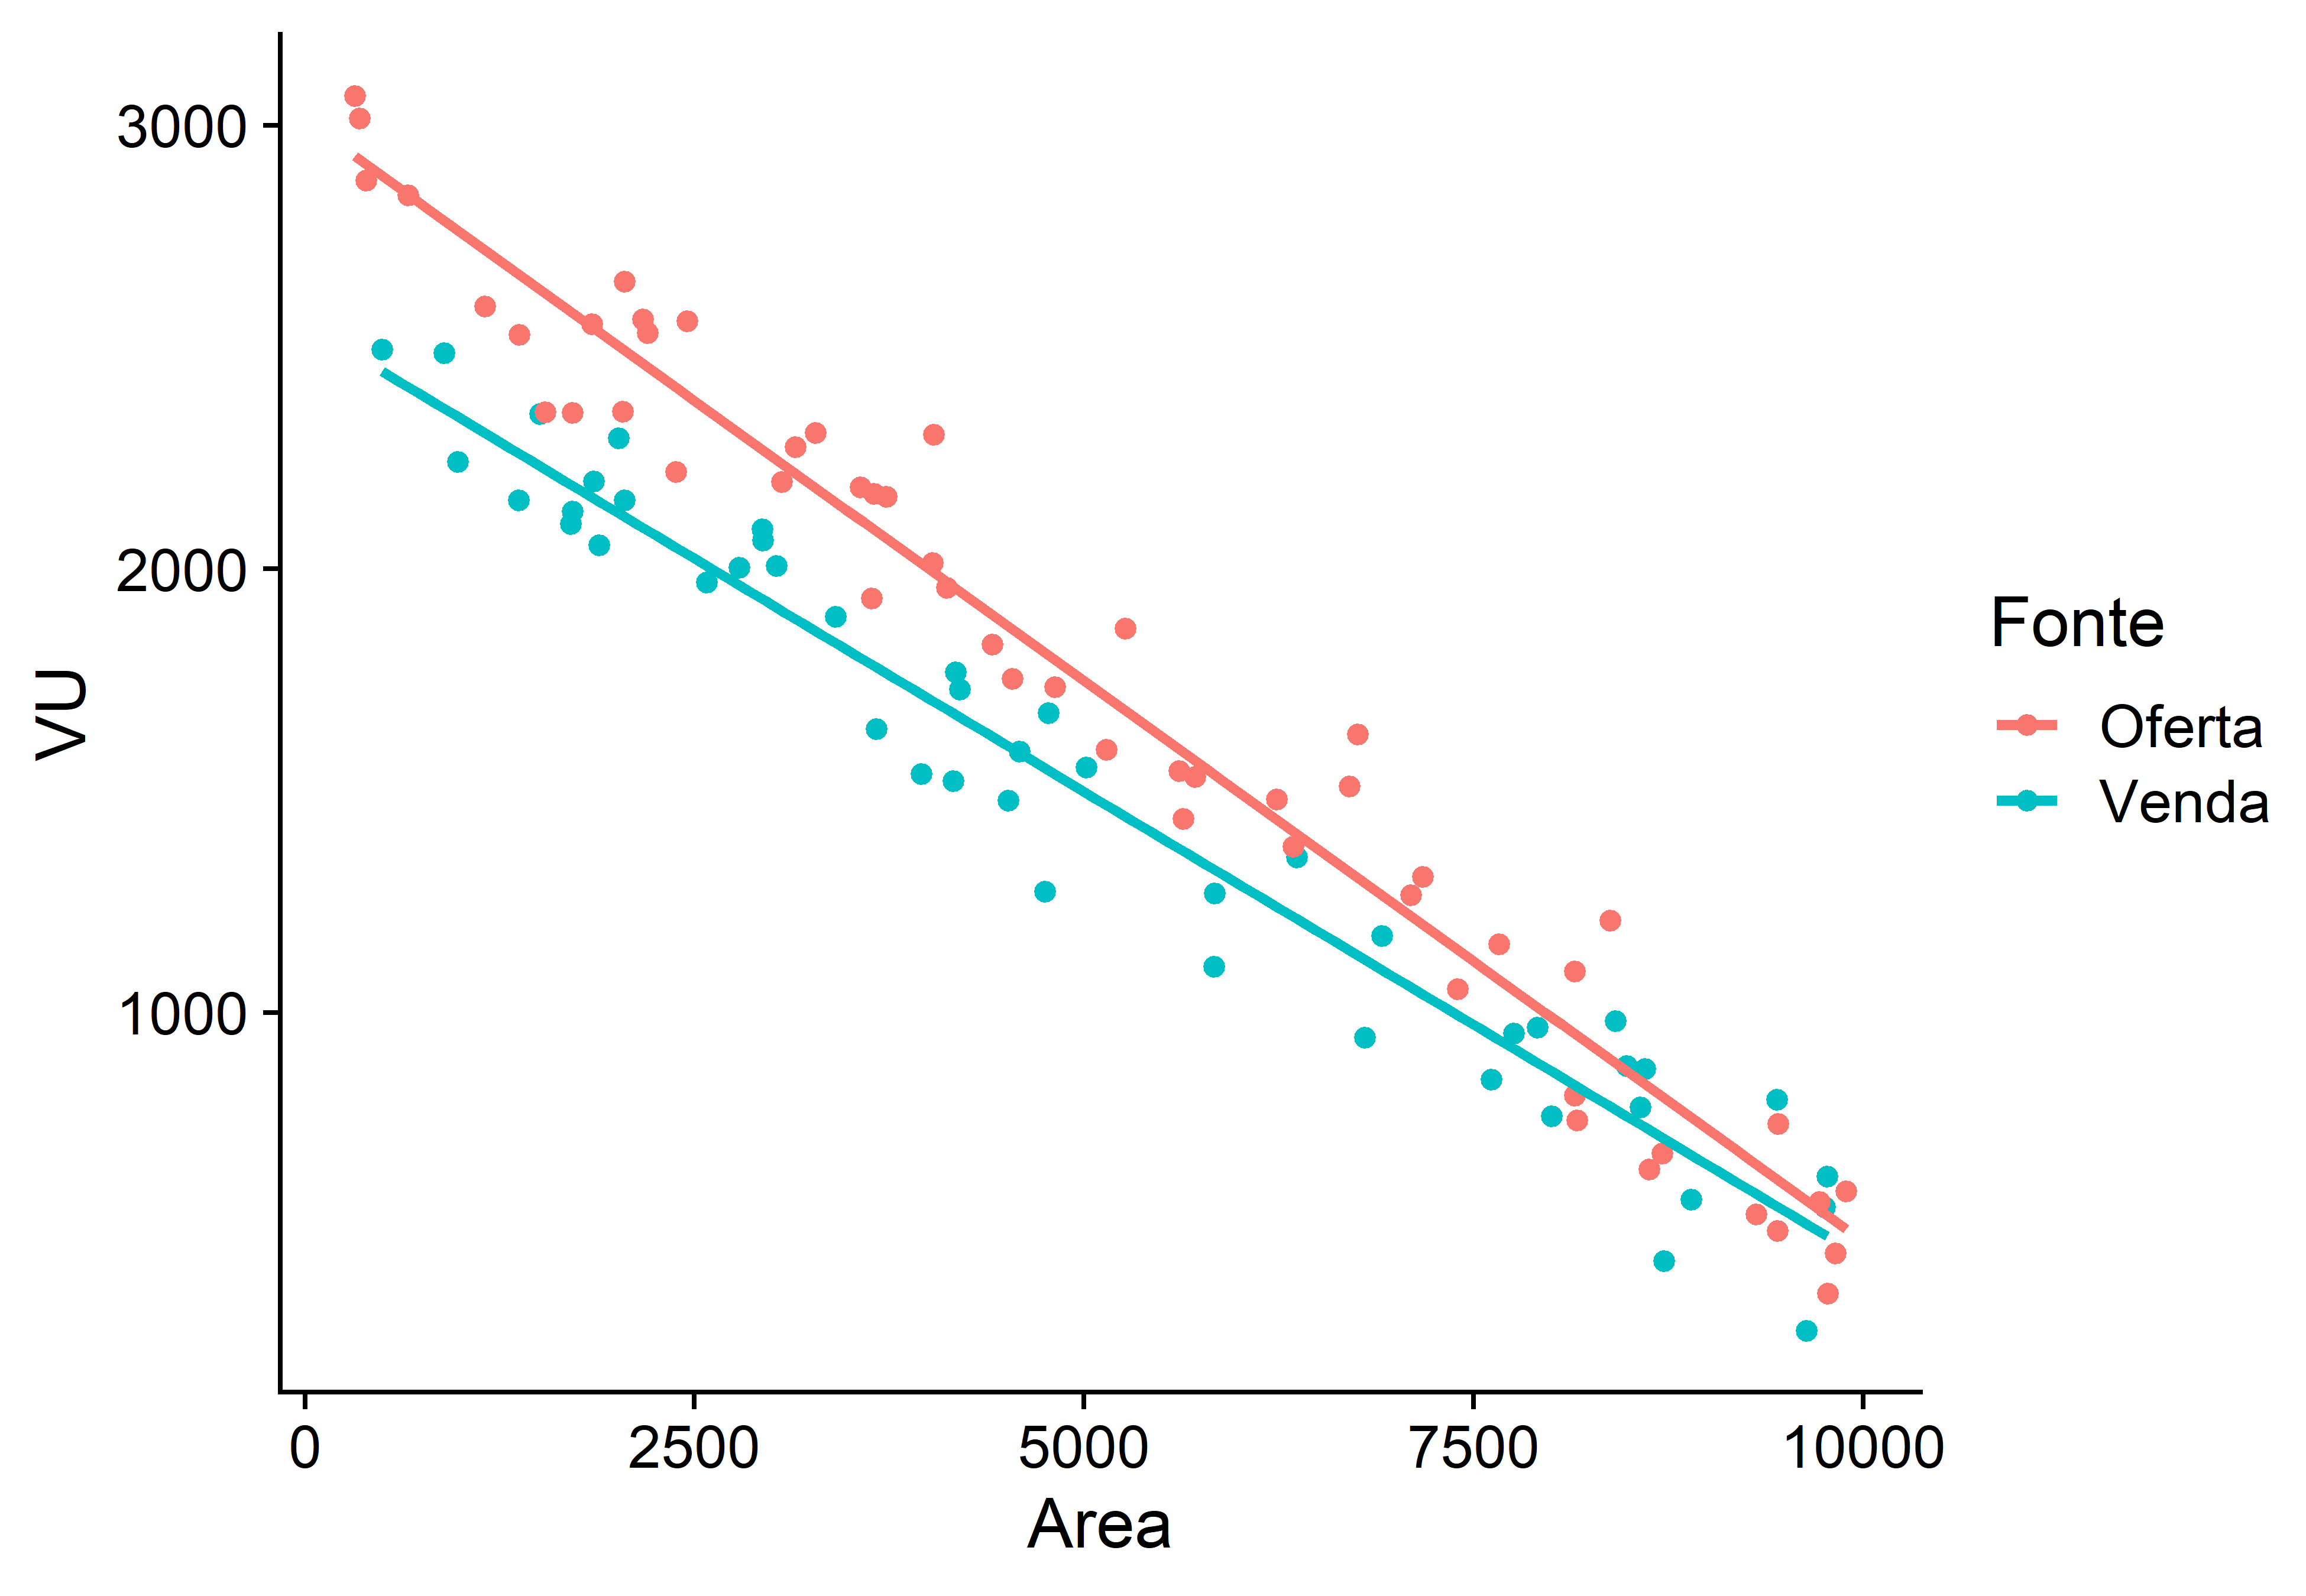
\includegraphics{./images/dados1-1.png}
\caption{Dados randômicos de oferta (em vermelho) e transação (em
verde)}
\end{figure}

Como é possível perceber já pela simples visualização gráfica dos dados,
um modelo de regressão que contemple o fator fonte ou fator oferta na
forma direta\footnote{Isto é, sem a utilização de transformação para a
  variável dependente.}, deverá fazê-lo por meio da adição de uma
interação entre a variável \(Fonte\) com as outras variáveis
explicativas do modelo.

Apenas para efeito ilustrativo, ajustou-se um modelo com a variável
\(Fonte\) na forma direta, sem a adição da interação entre ela e a
variável explicativa. O modelo mostrou-se bem ajustado.

\begin{figure}
\centering
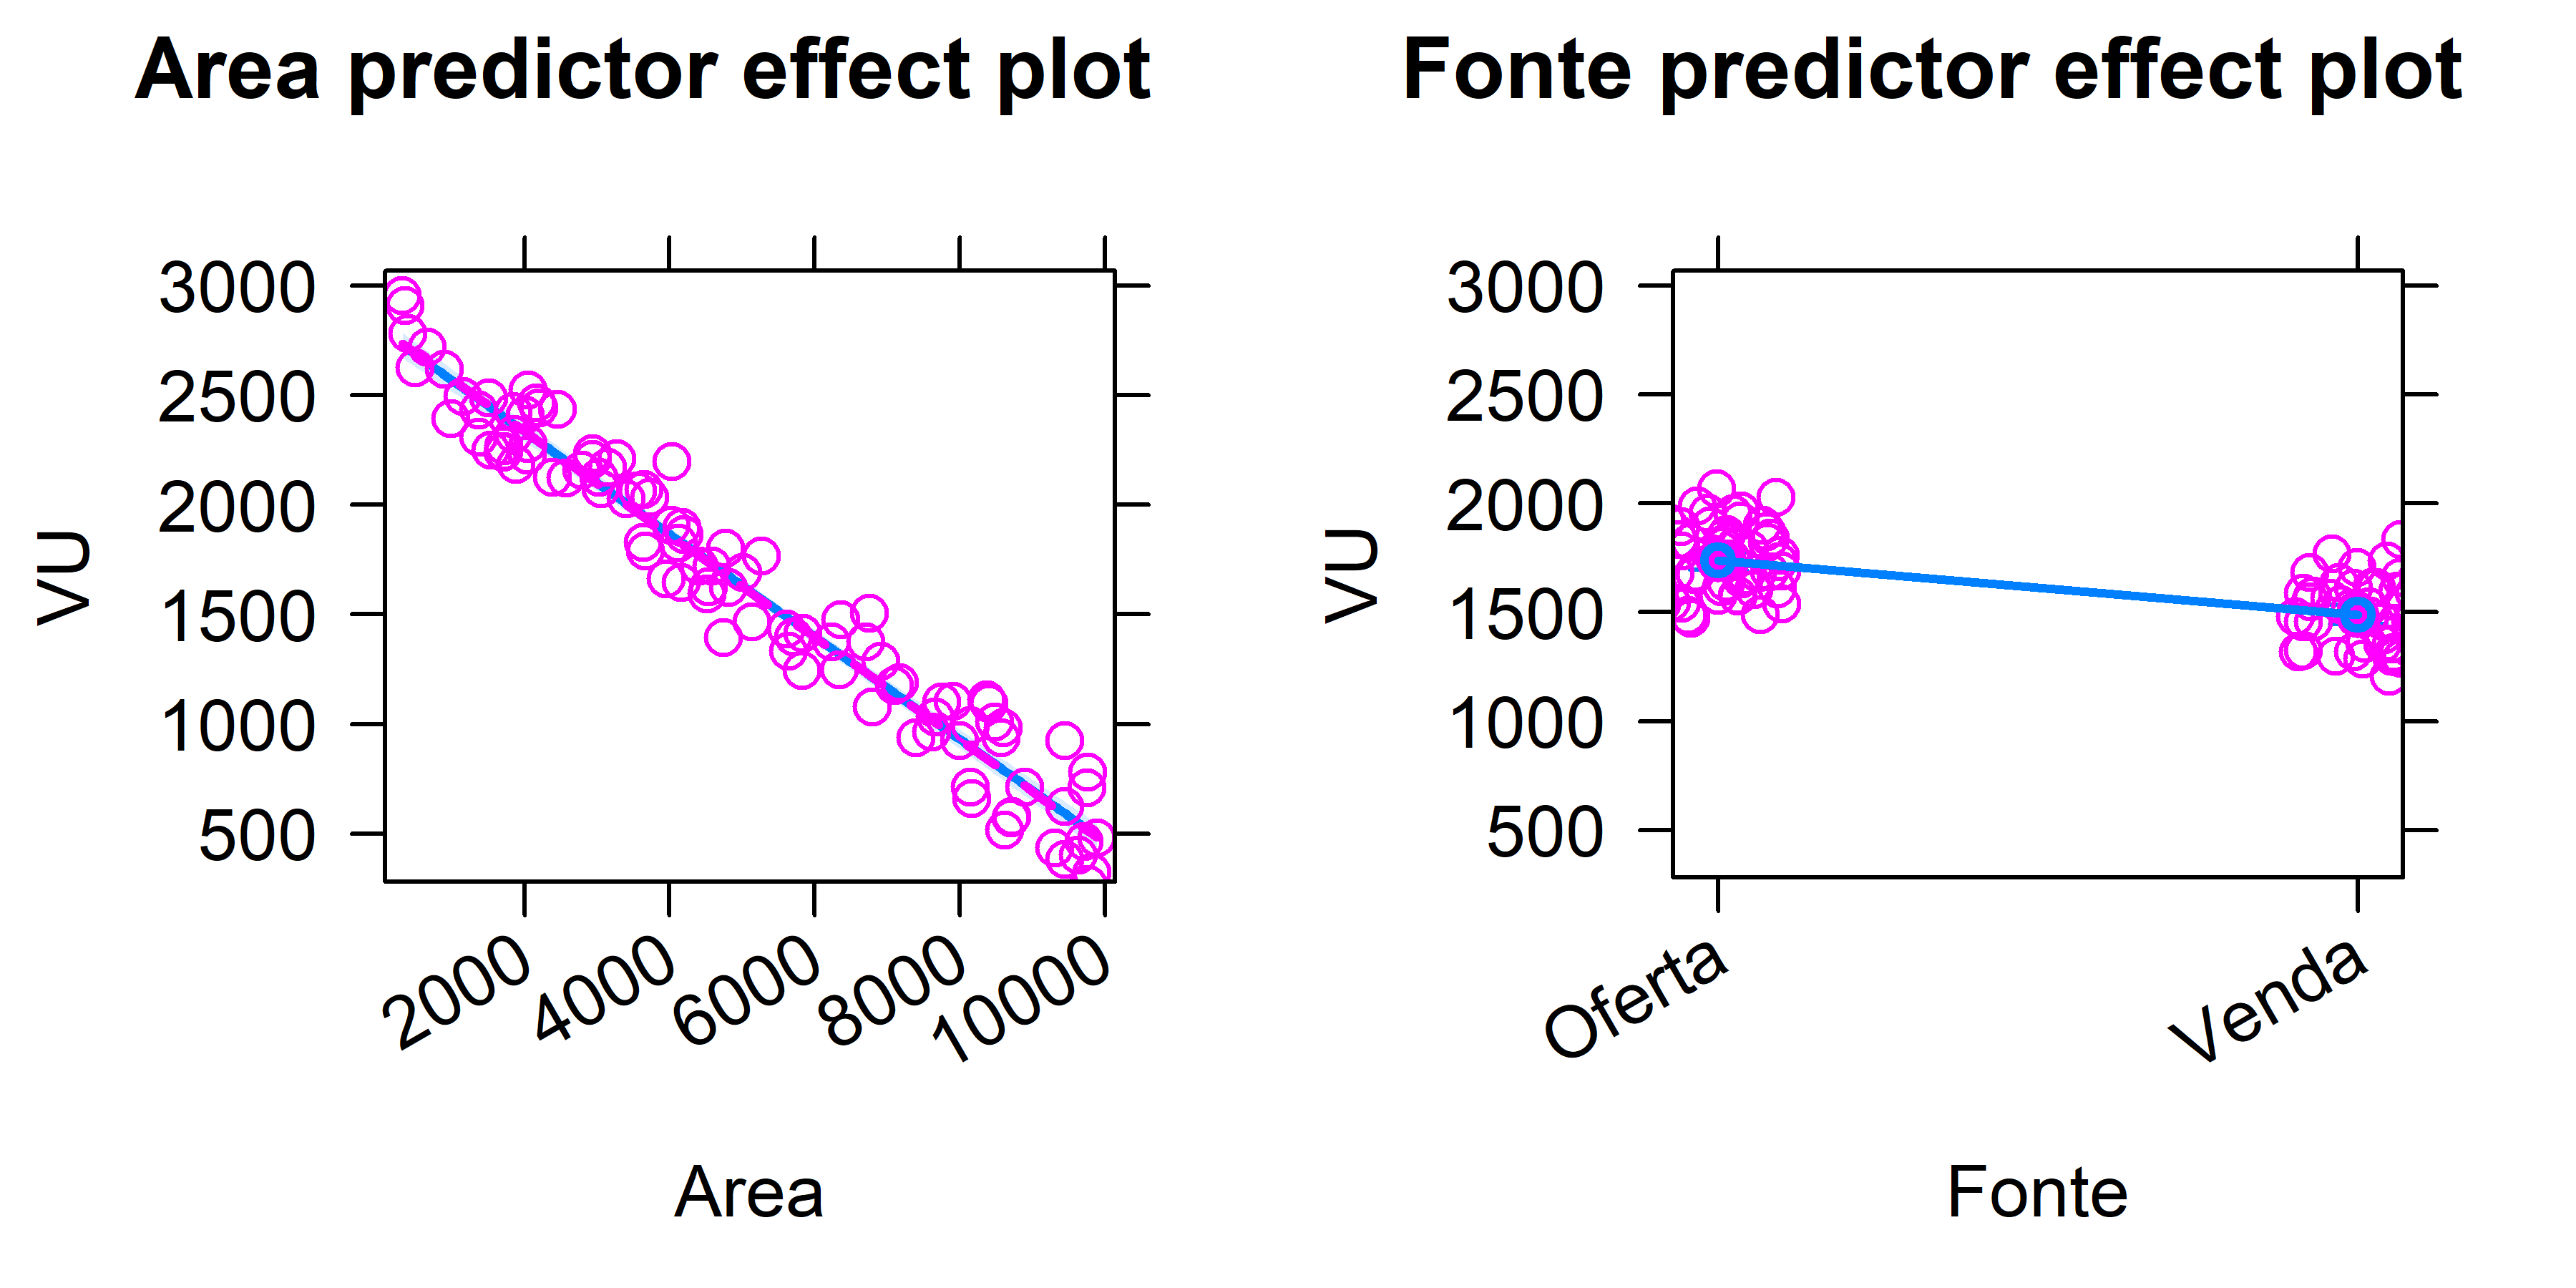
\includegraphics{./images/wrongModel-1.png}
\caption{Fator oferta na forma direta. Má especificação do modelo.}
\end{figure}

\begin{figure}[H]
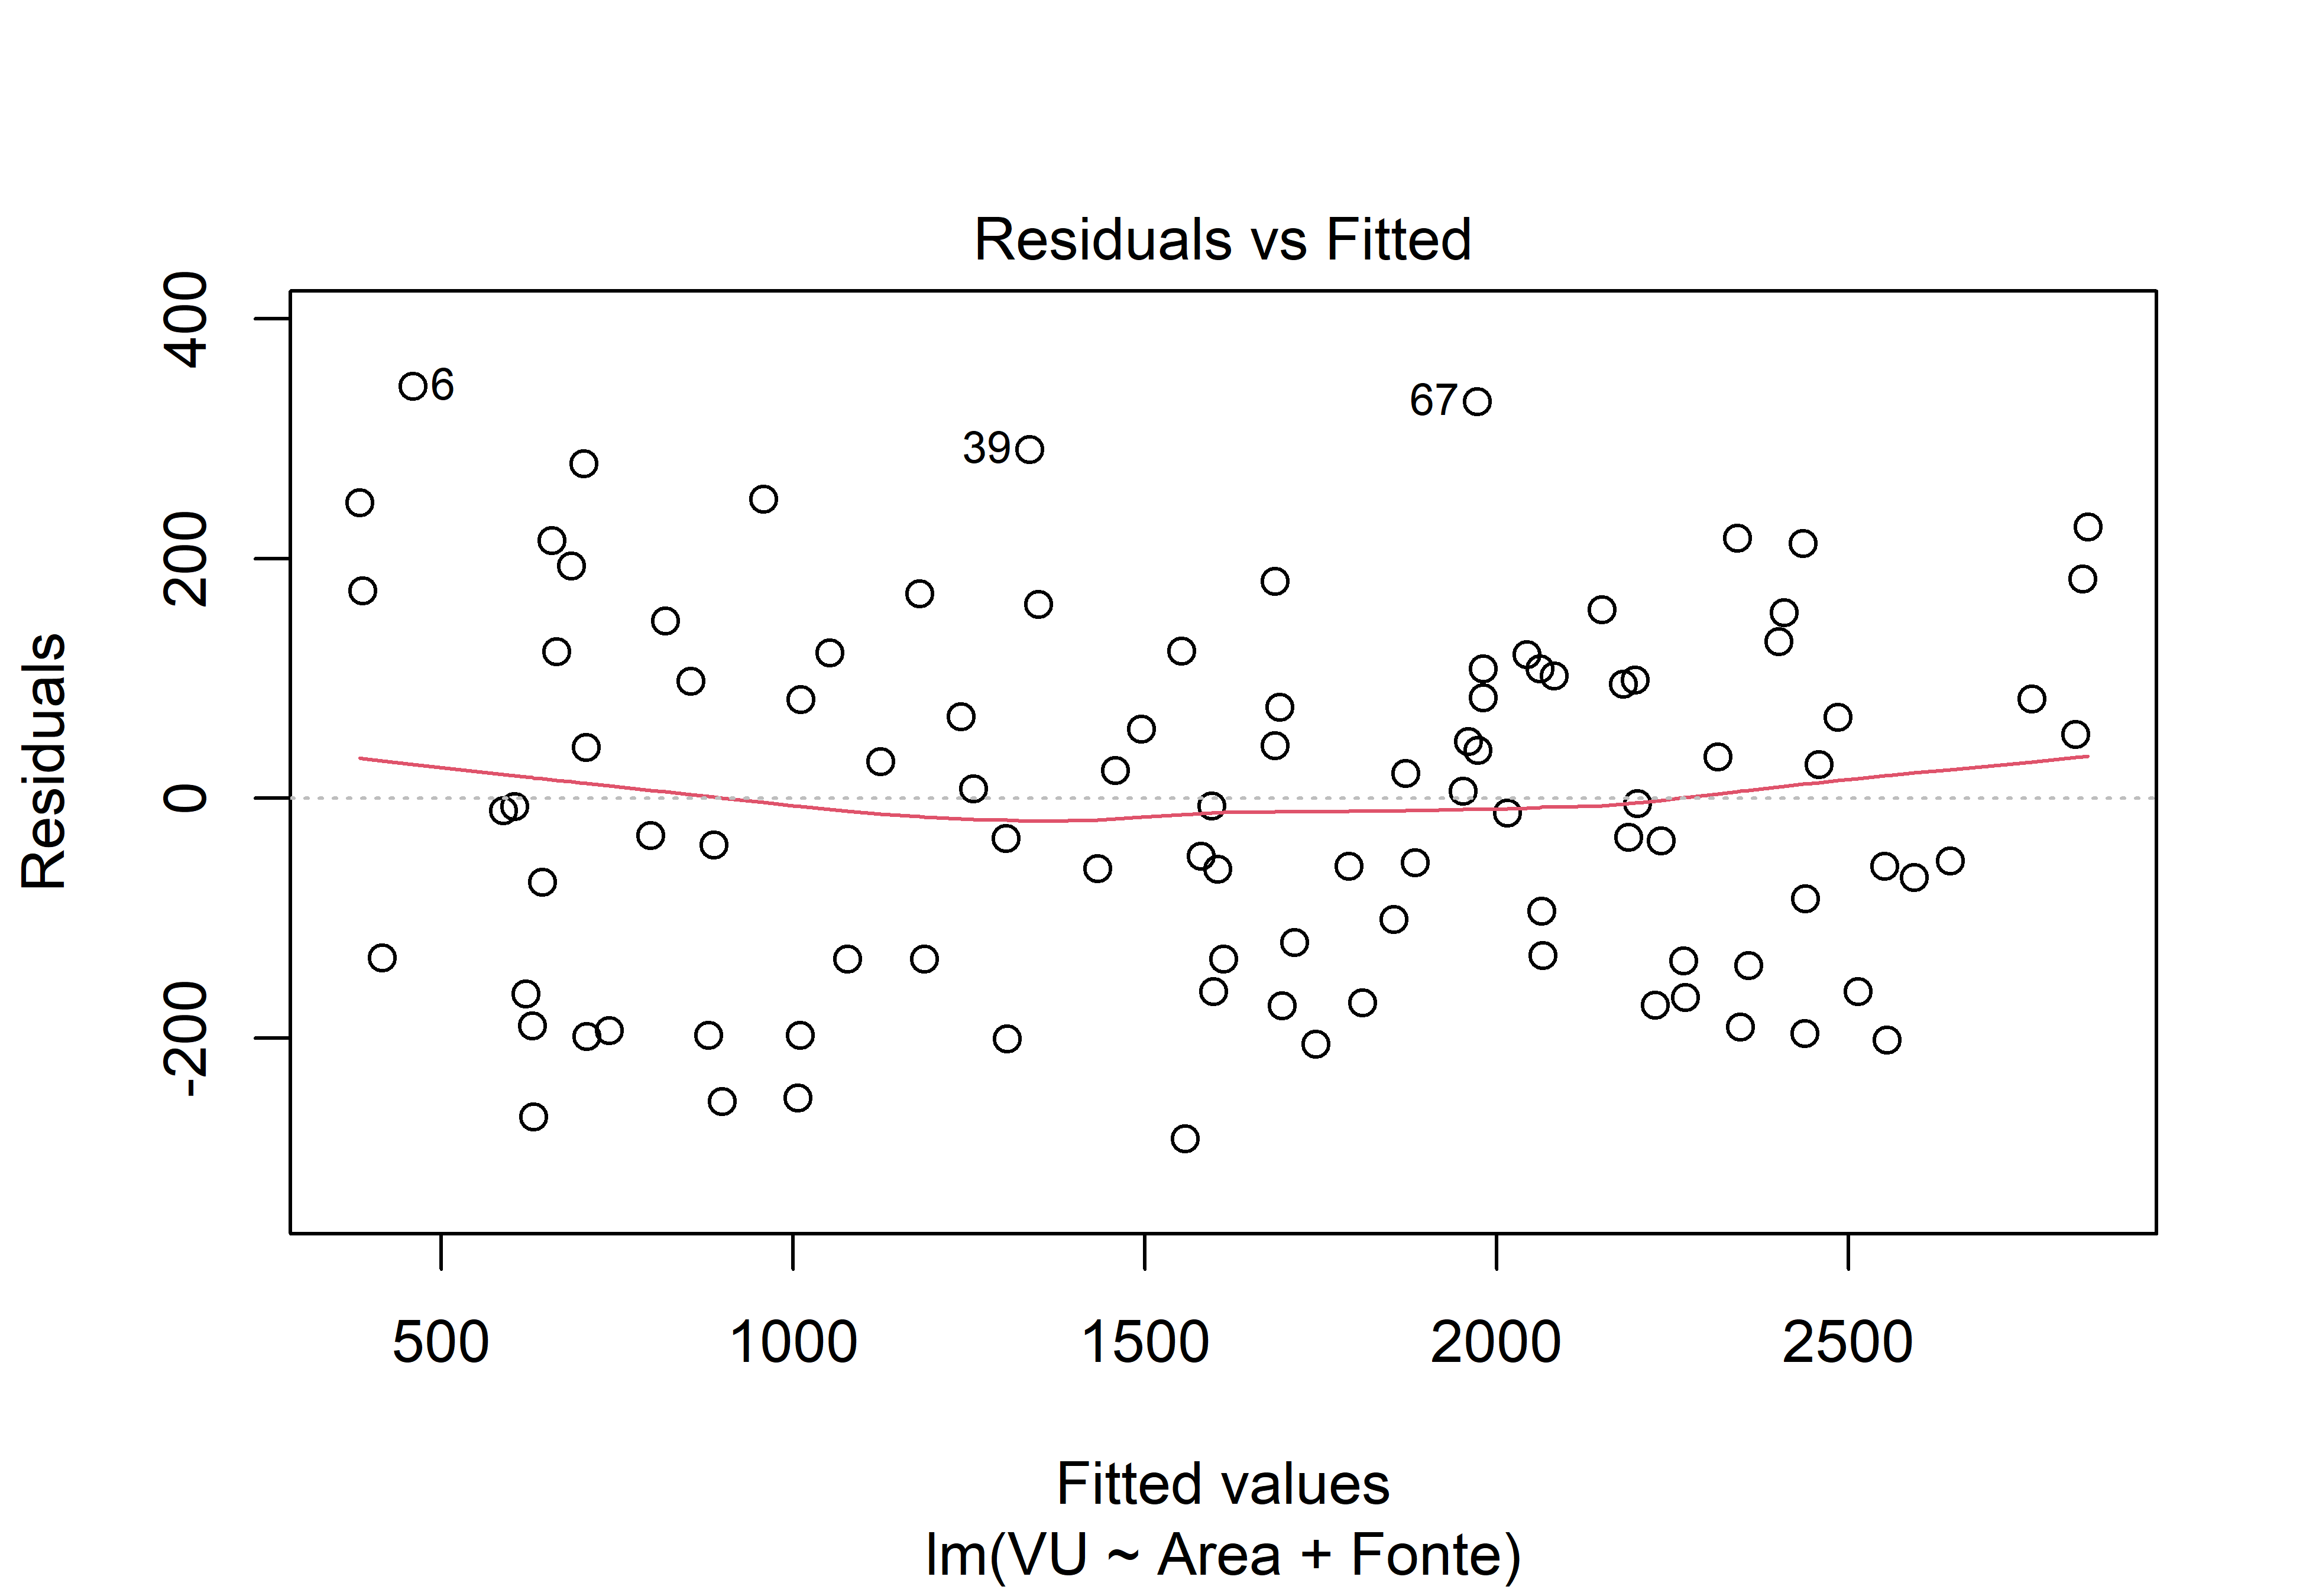
\includegraphics[width=0.5\linewidth]{./images/fitPlot-1} 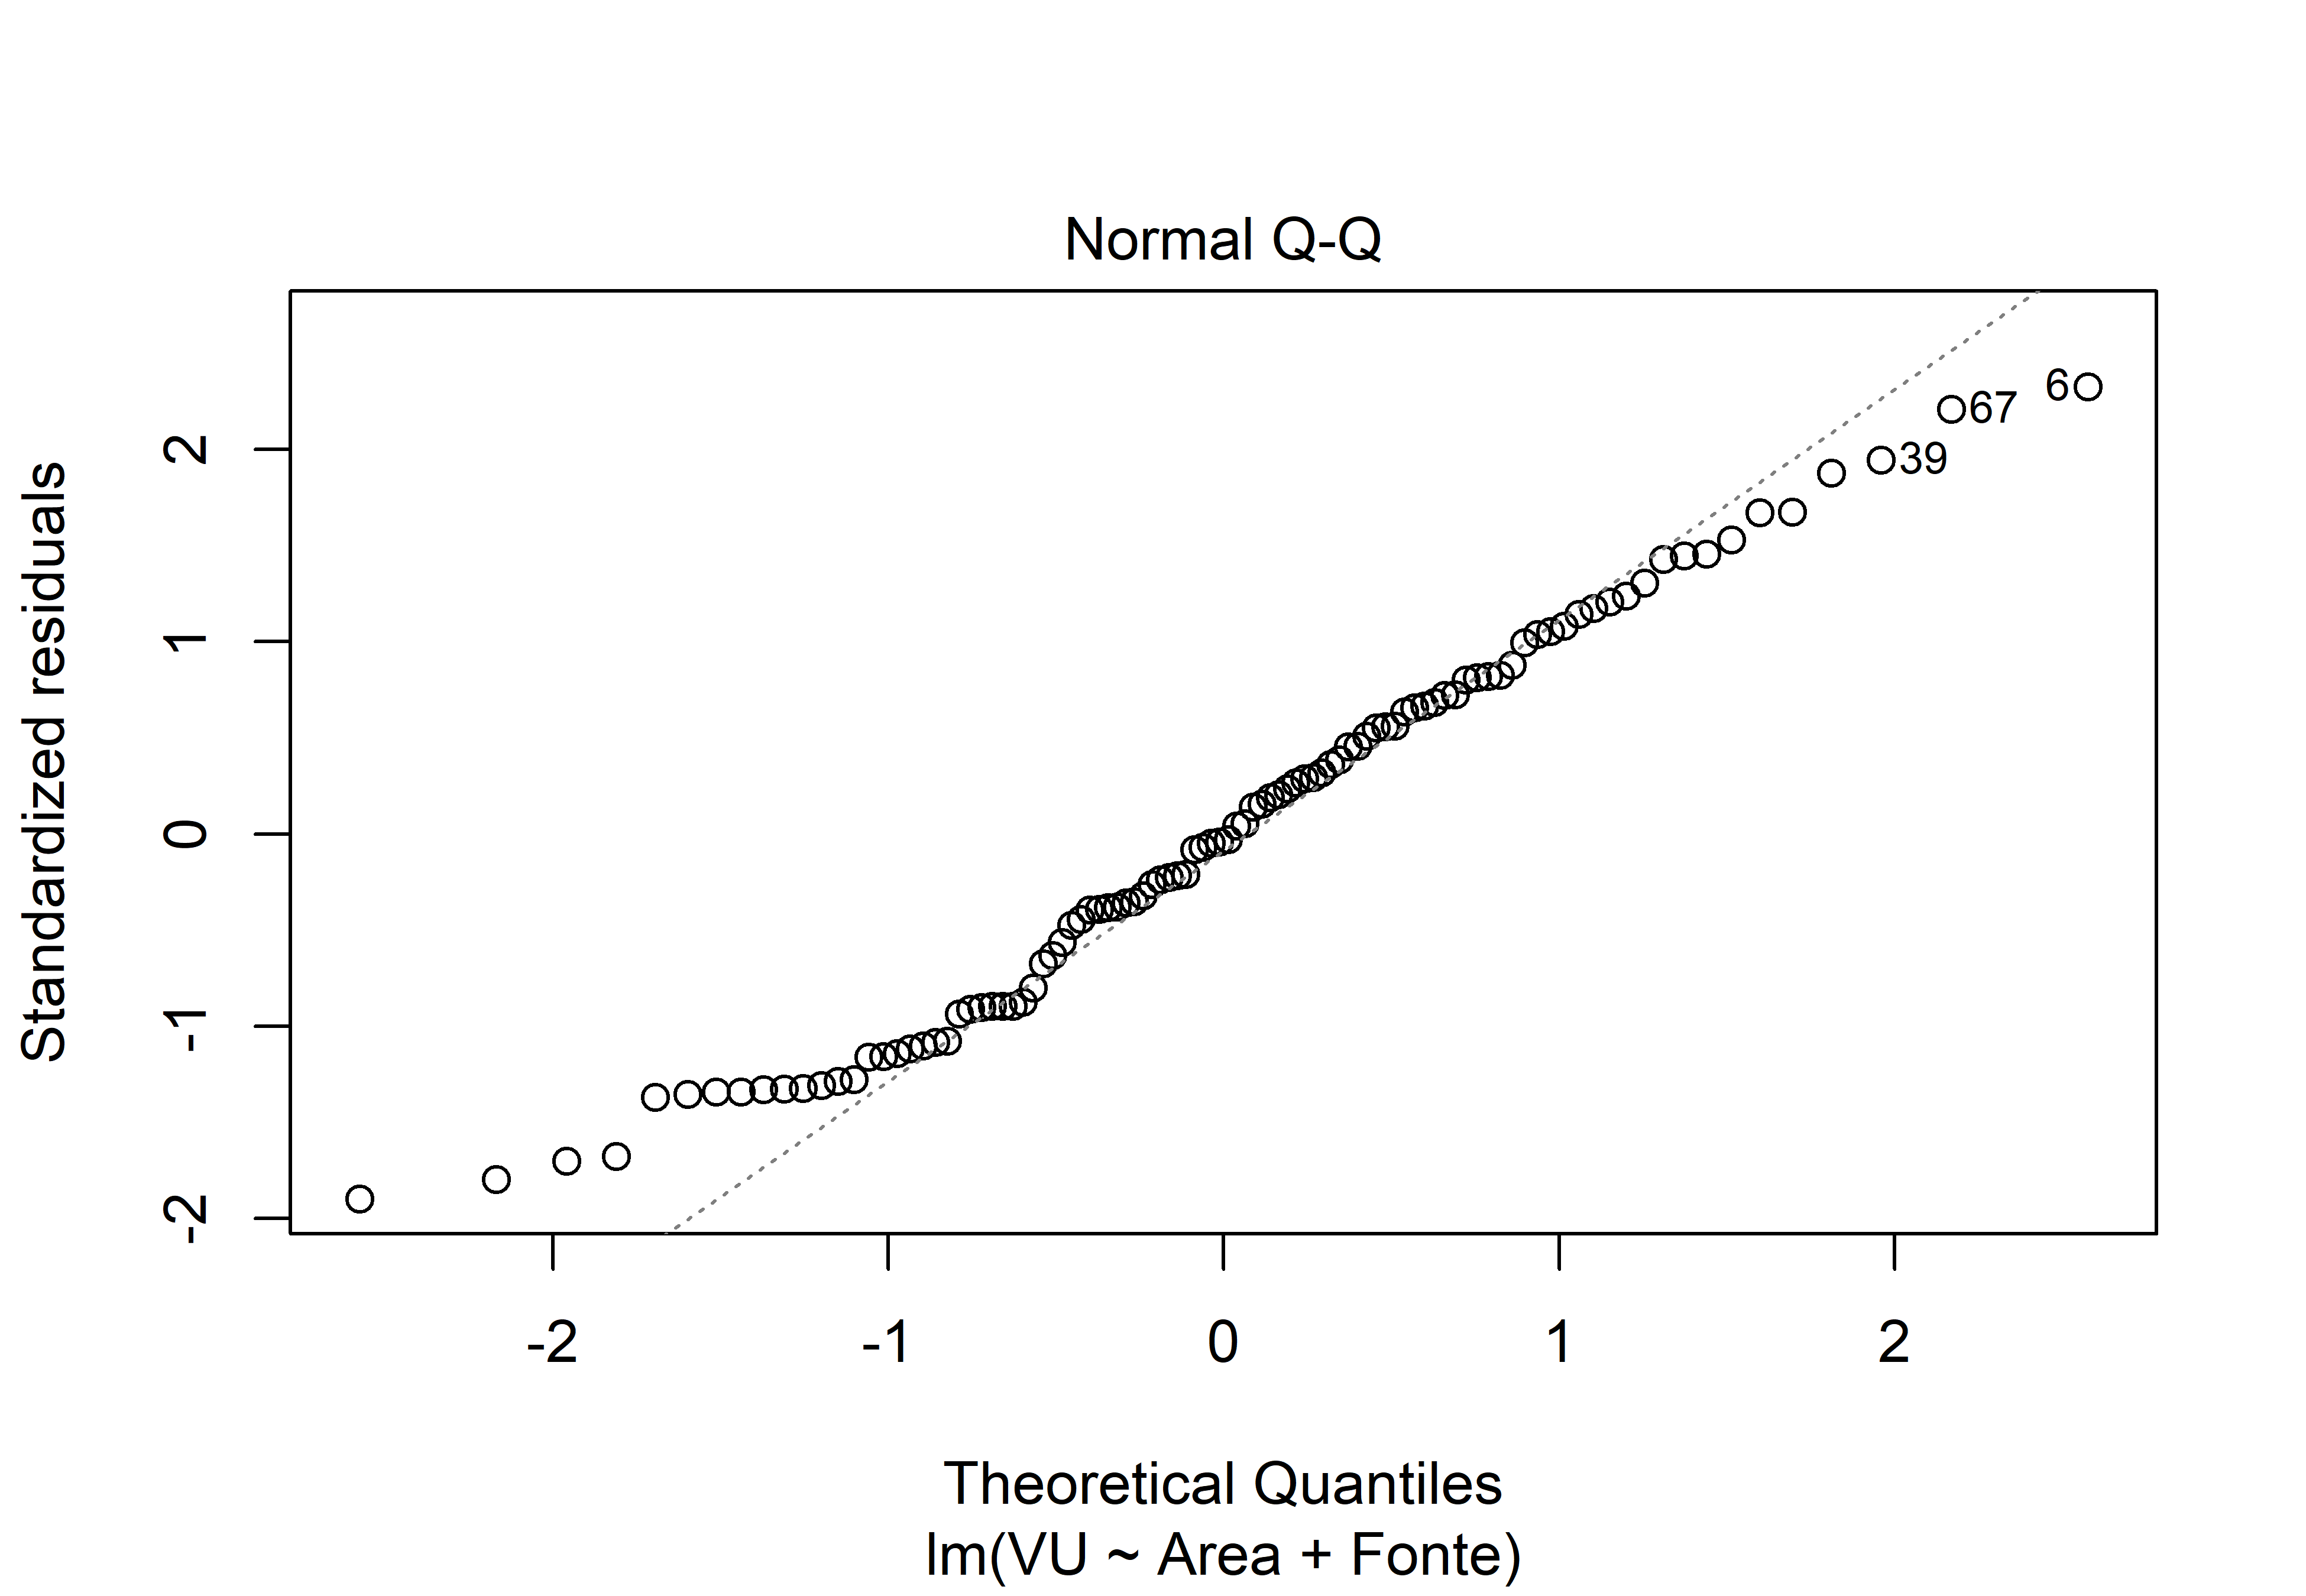
\includegraphics[width=0.5\linewidth]{./images/fitPlot-2} 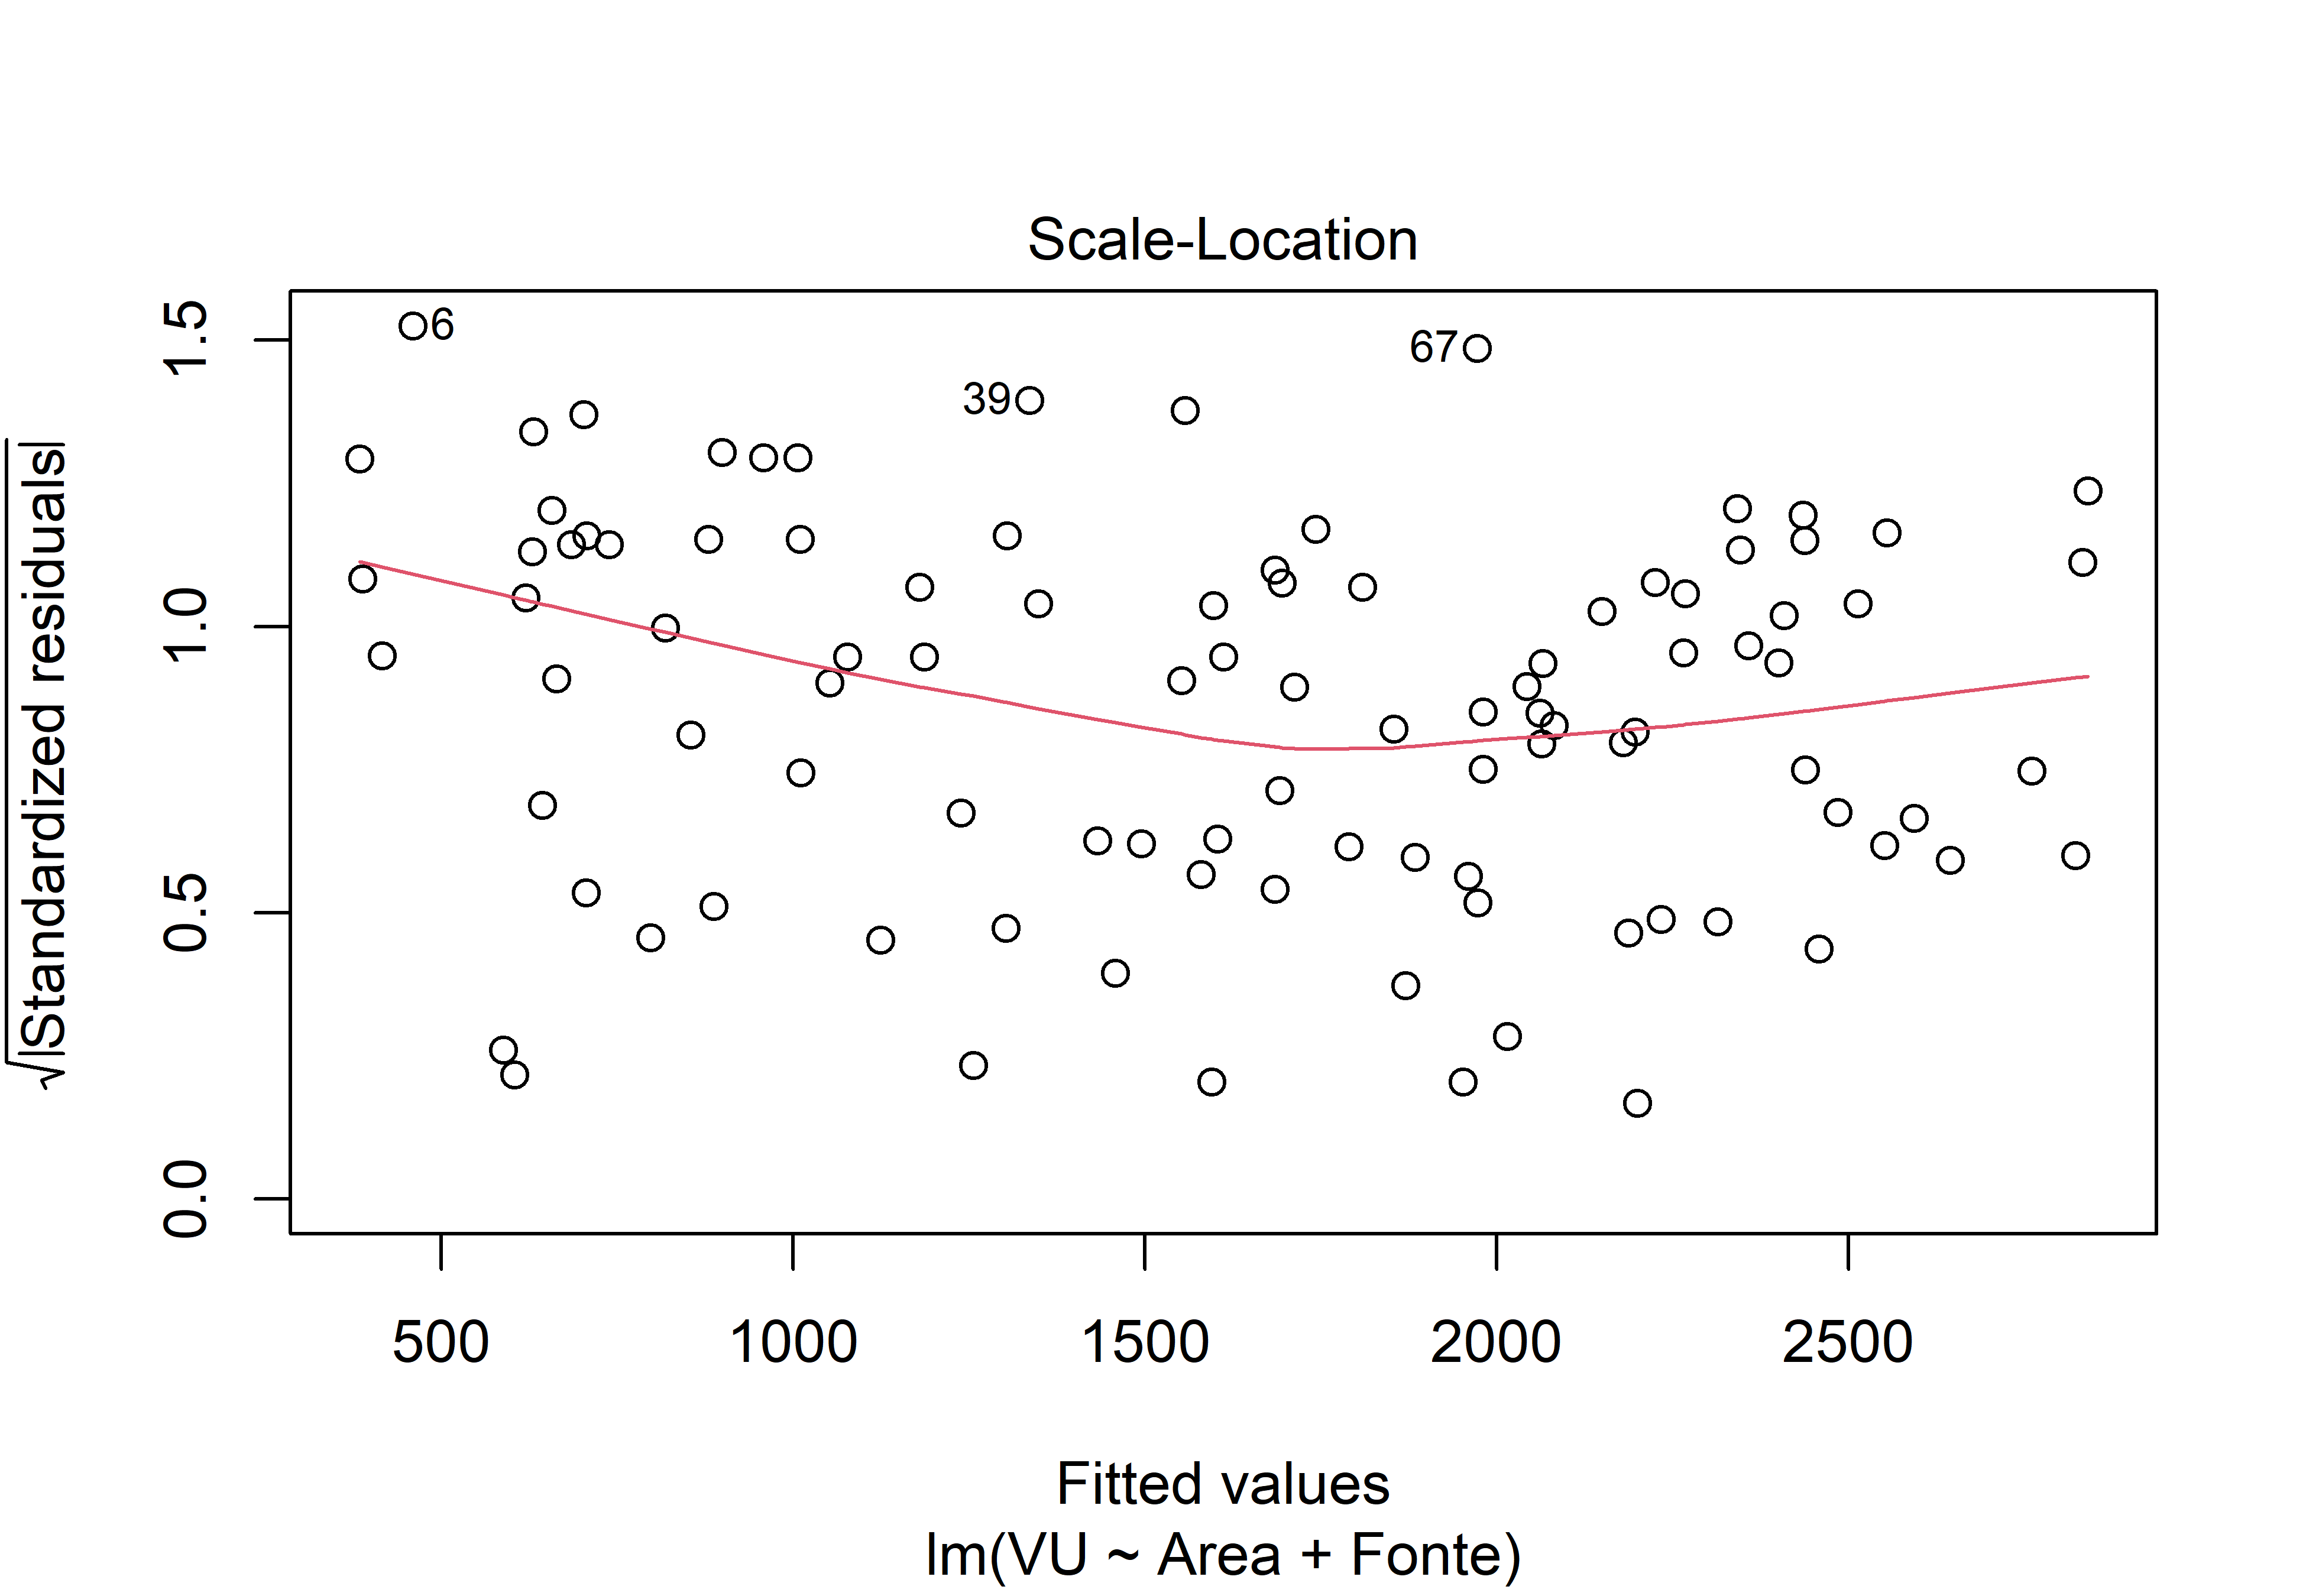
\includegraphics[width=0.5\linewidth]{./images/fitPlot-3} 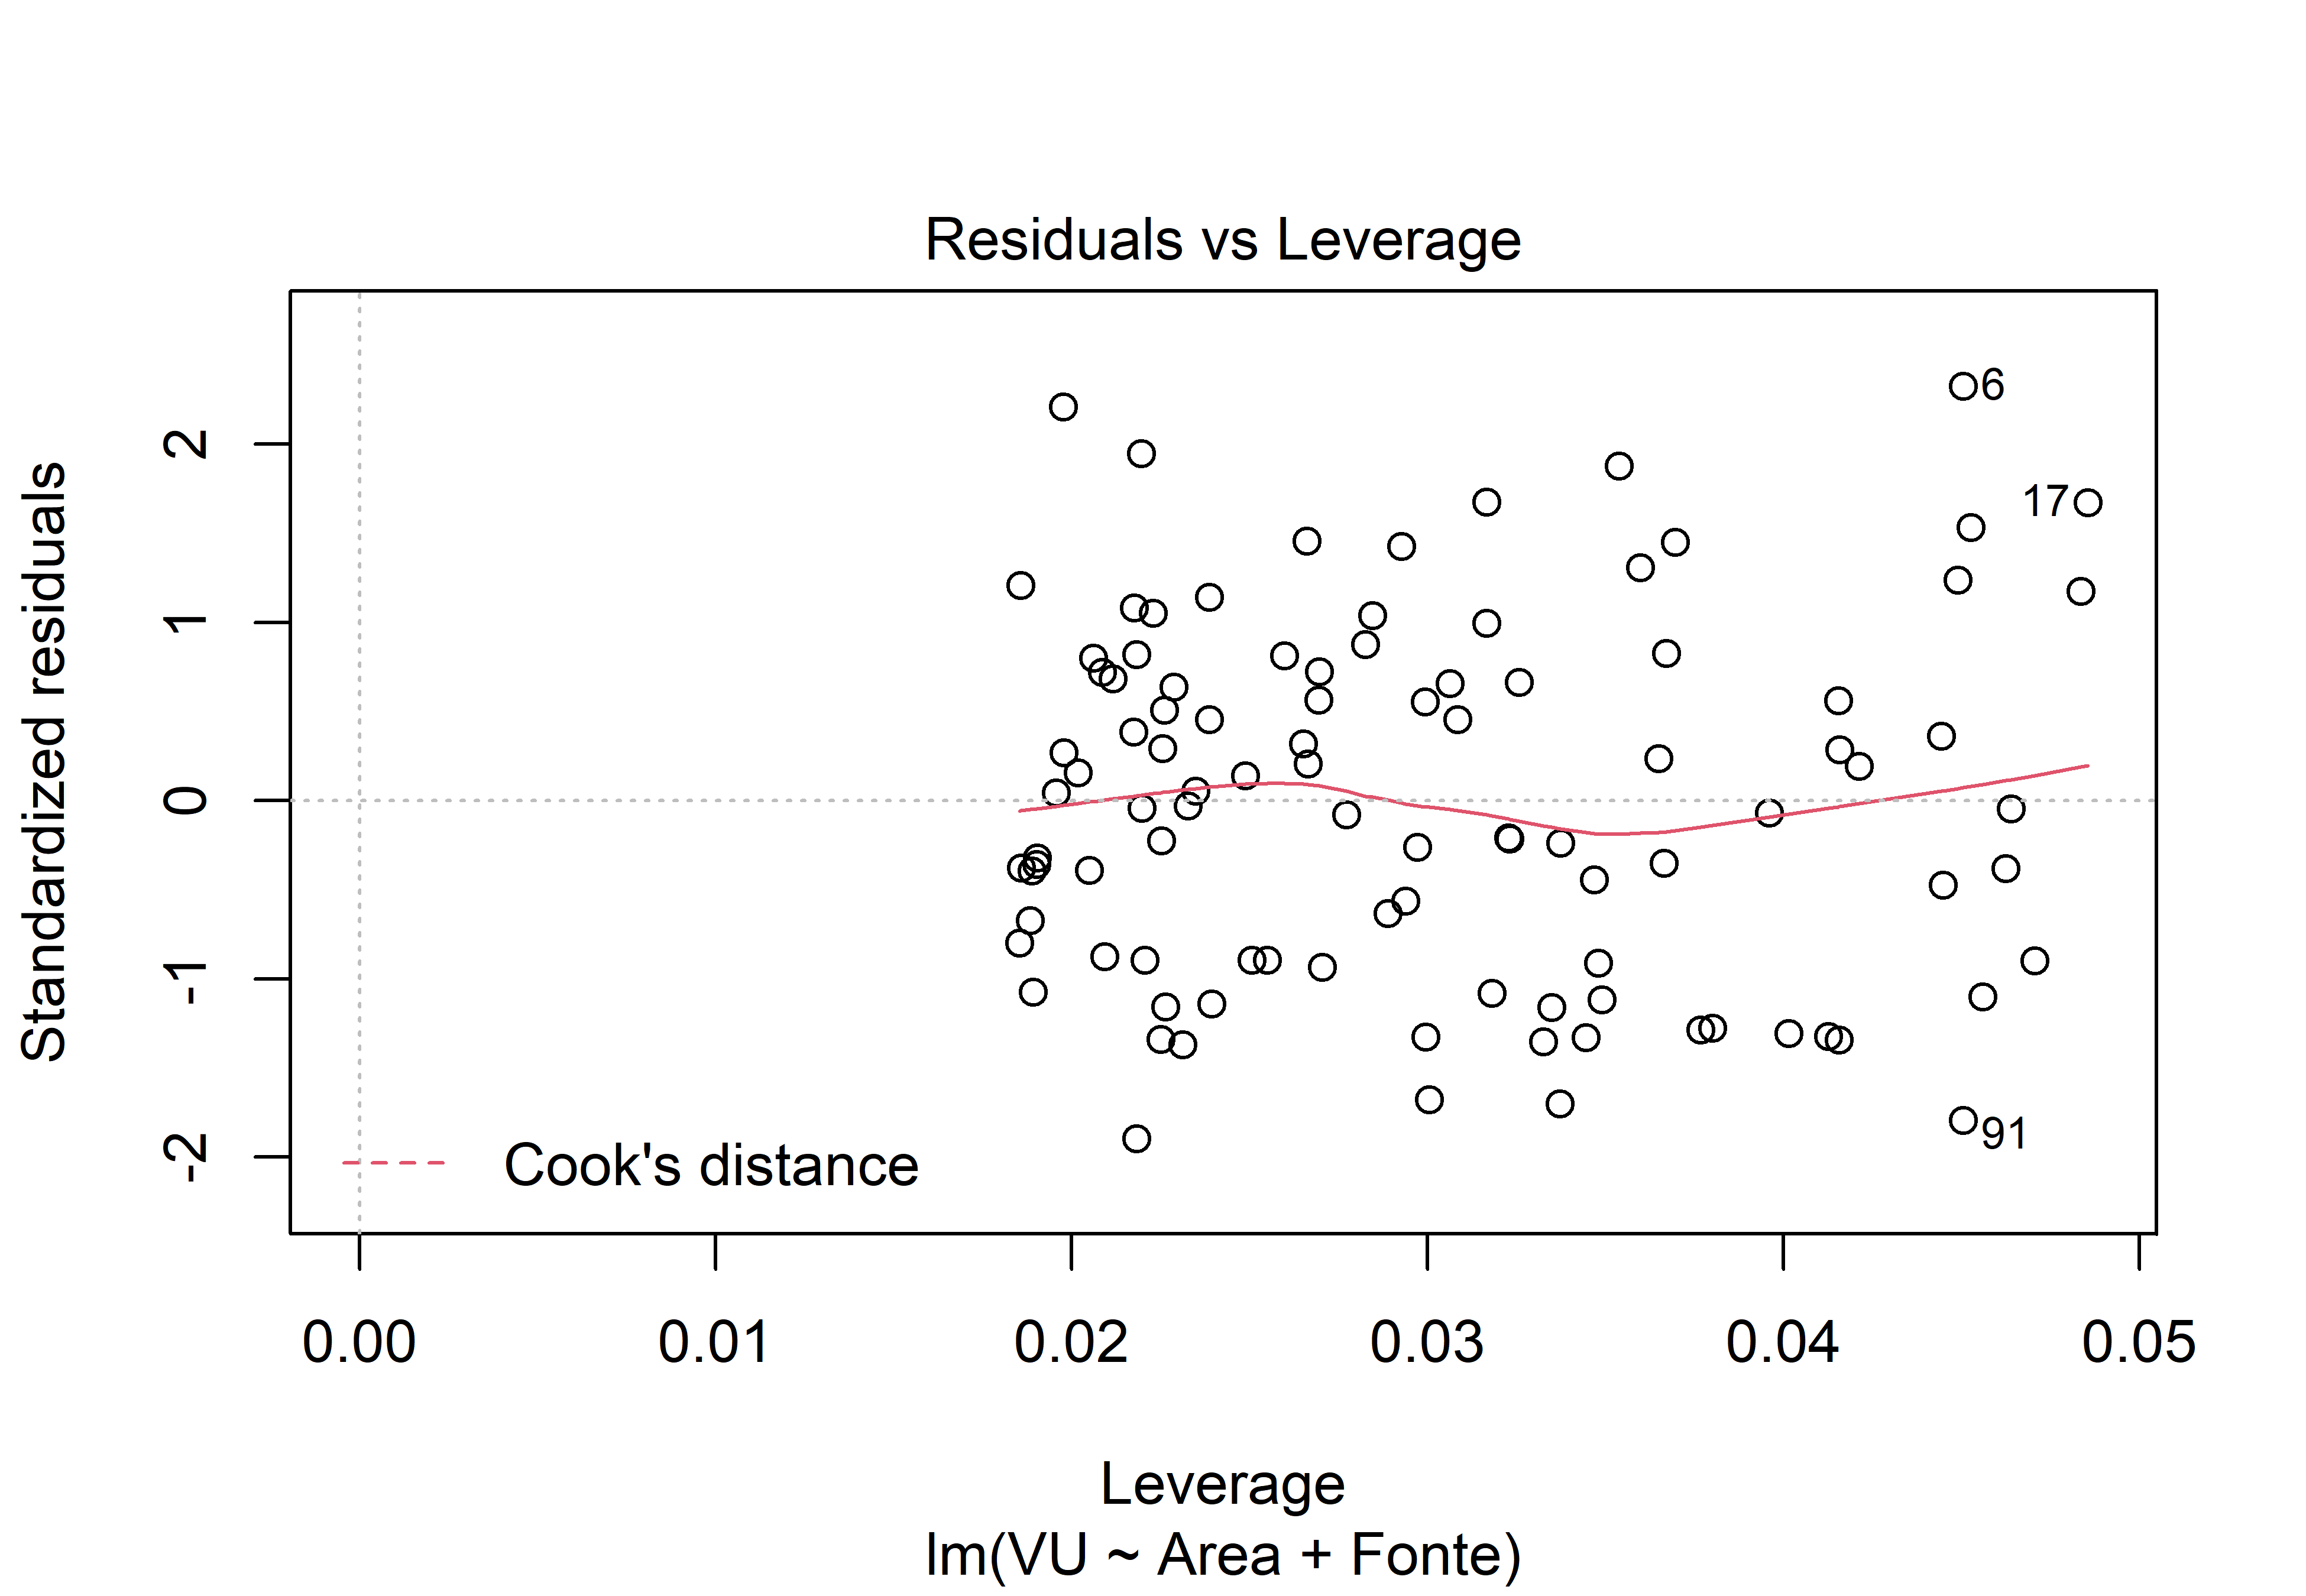
\includegraphics[width=0.5\linewidth]{./images/fitPlot-4} \caption{Diagnóstico do modelo mau especificado na forma direta.}\label{fig:fitPlot}
\end{figure}

Com esta formulação, o desconto é constante ao longo de todo o modelo. É
possível verificar a falha na especificação do modelo de forma gráfica,
pela análise dos gráficos diagnósticos da Figura \ref{fig:fitPlot}, ou
através do teste de Breusch-Pagan.

\begin{verbatim}
## 
##  studentized Breusch-Pagan test
## 
## data:  fit
## BP = 6.4355, df = 2, p-value = 0.04005
\end{verbatim}

Com o ajuste correto do modelo, com a adição da interação entre a
variável \(Fonte\) e a variável explicativa \(Area\), a
heteroscedasticidade desaparece.

\begin{figure}
\centering
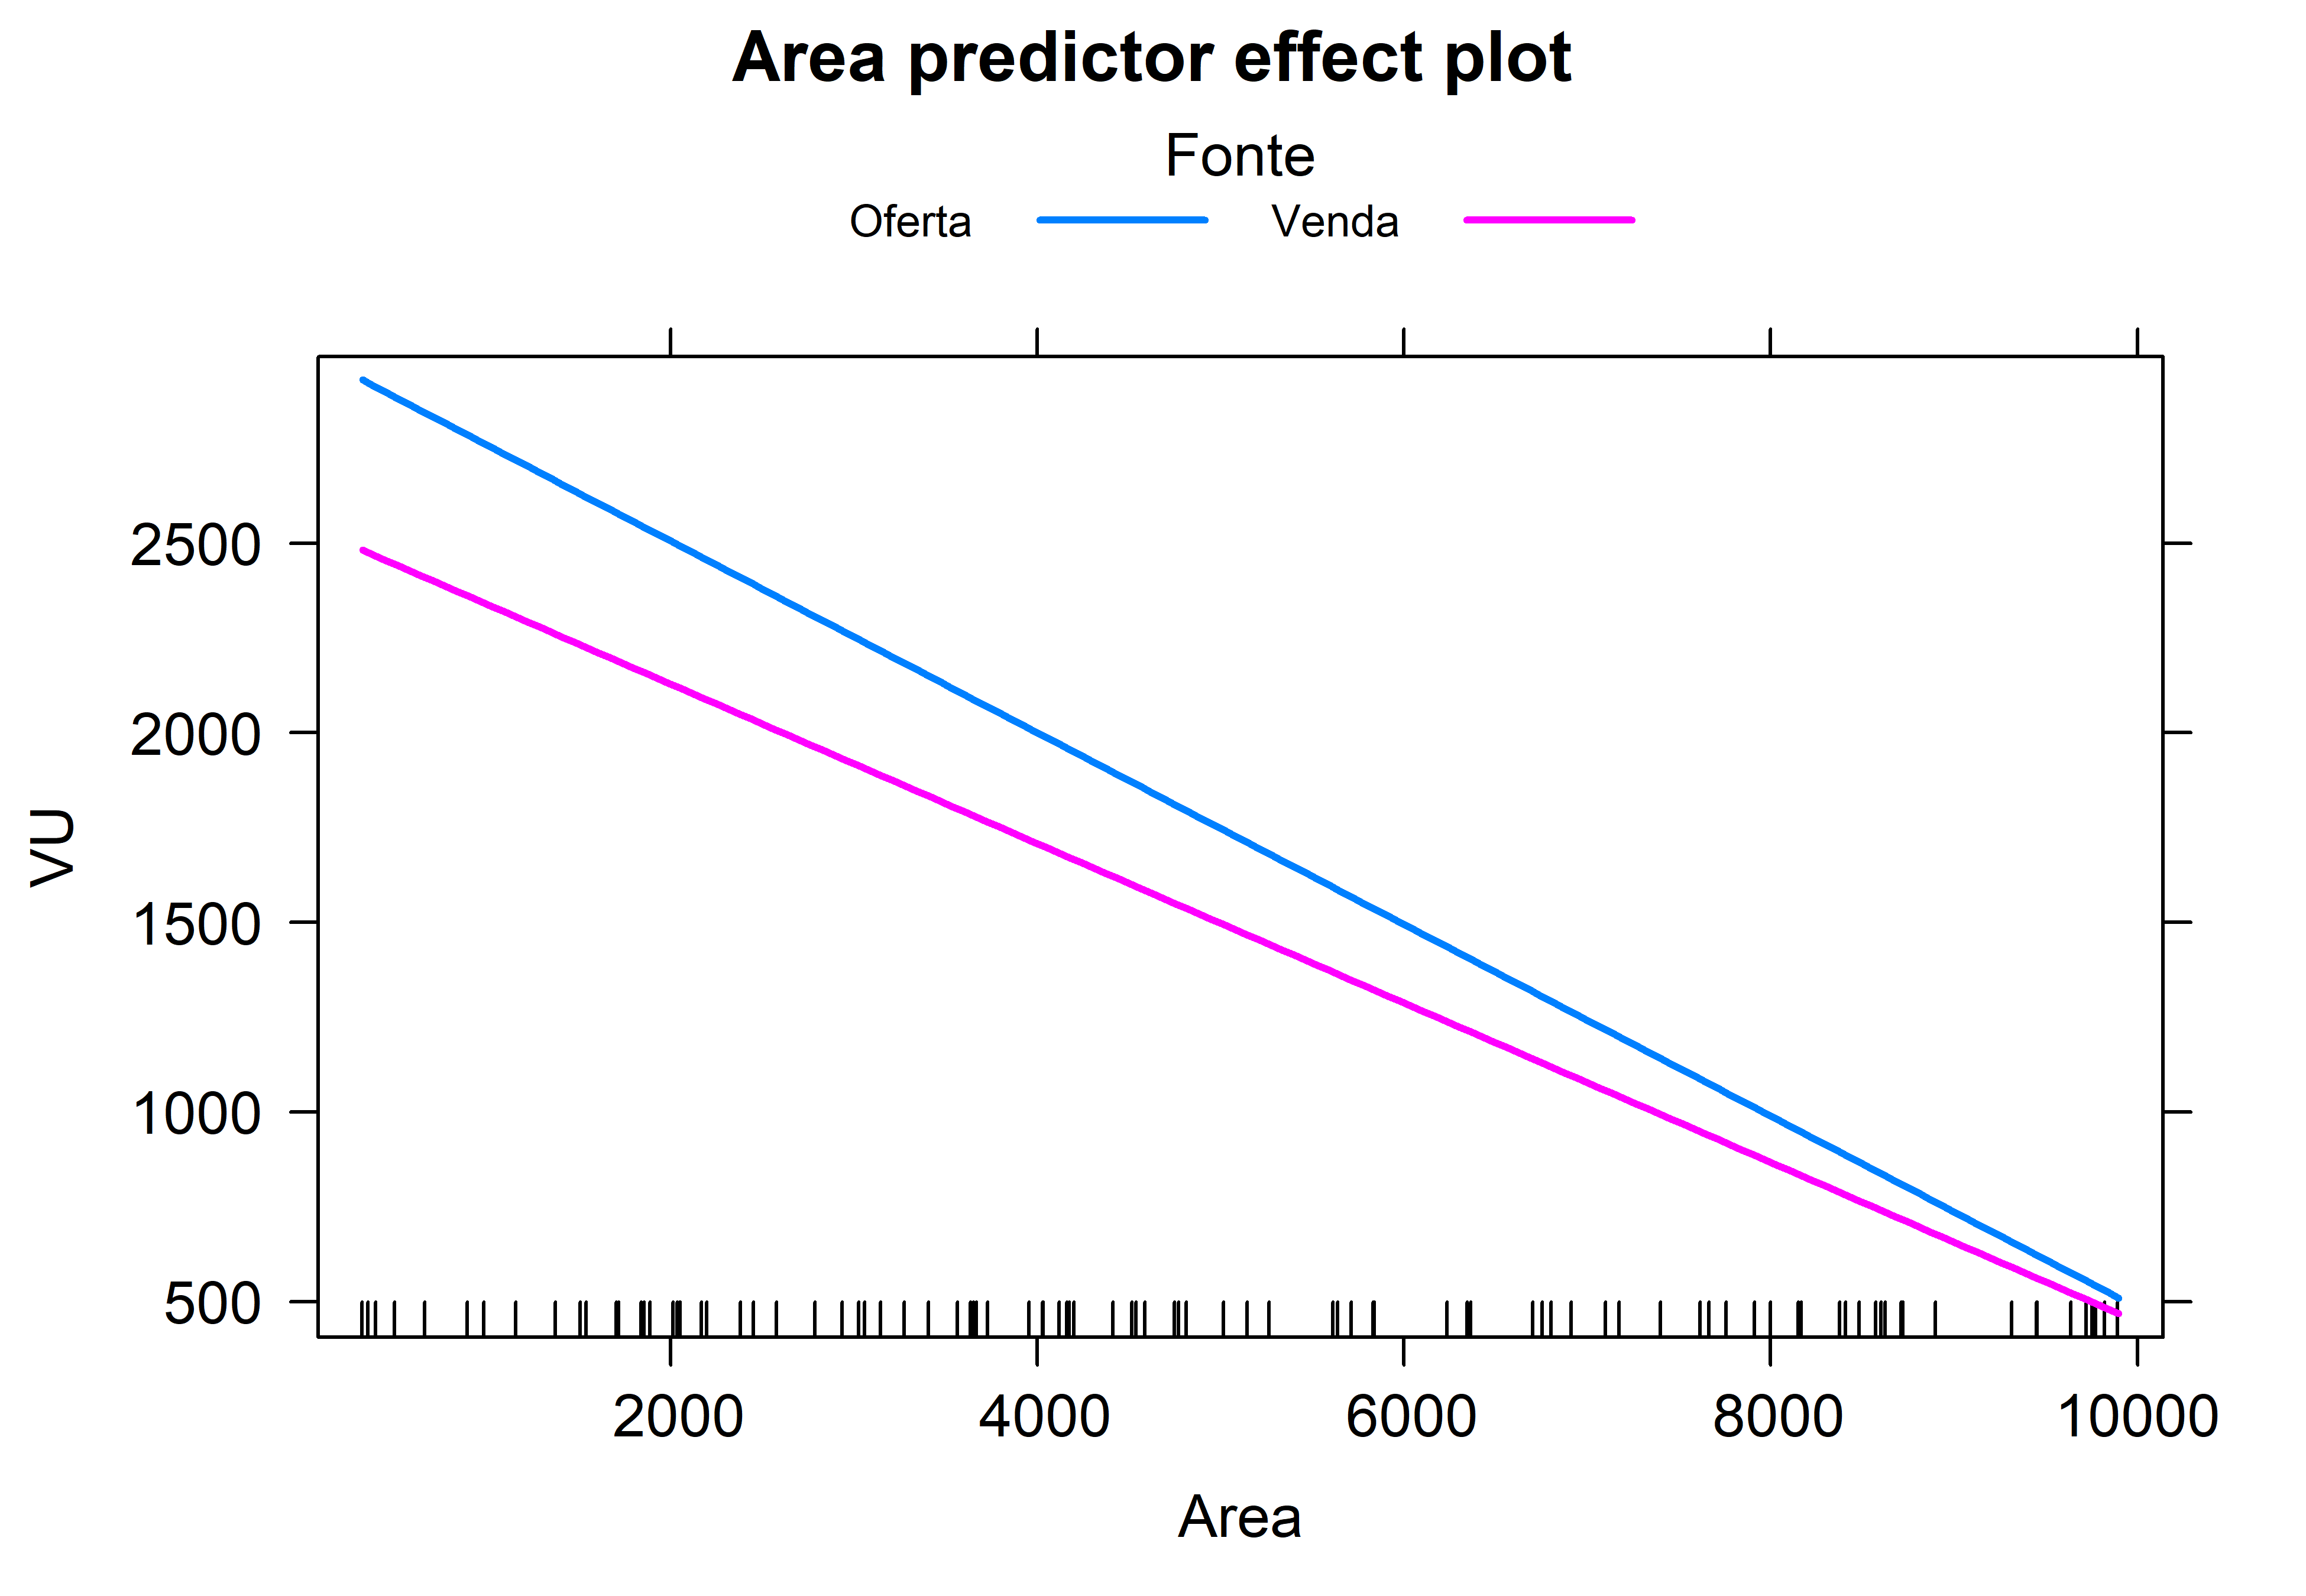
\includegraphics{./images/rightModel-1.png}
\caption{Fator oferta na forma direta. Modelo especificado
corretamente.}
\end{figure}

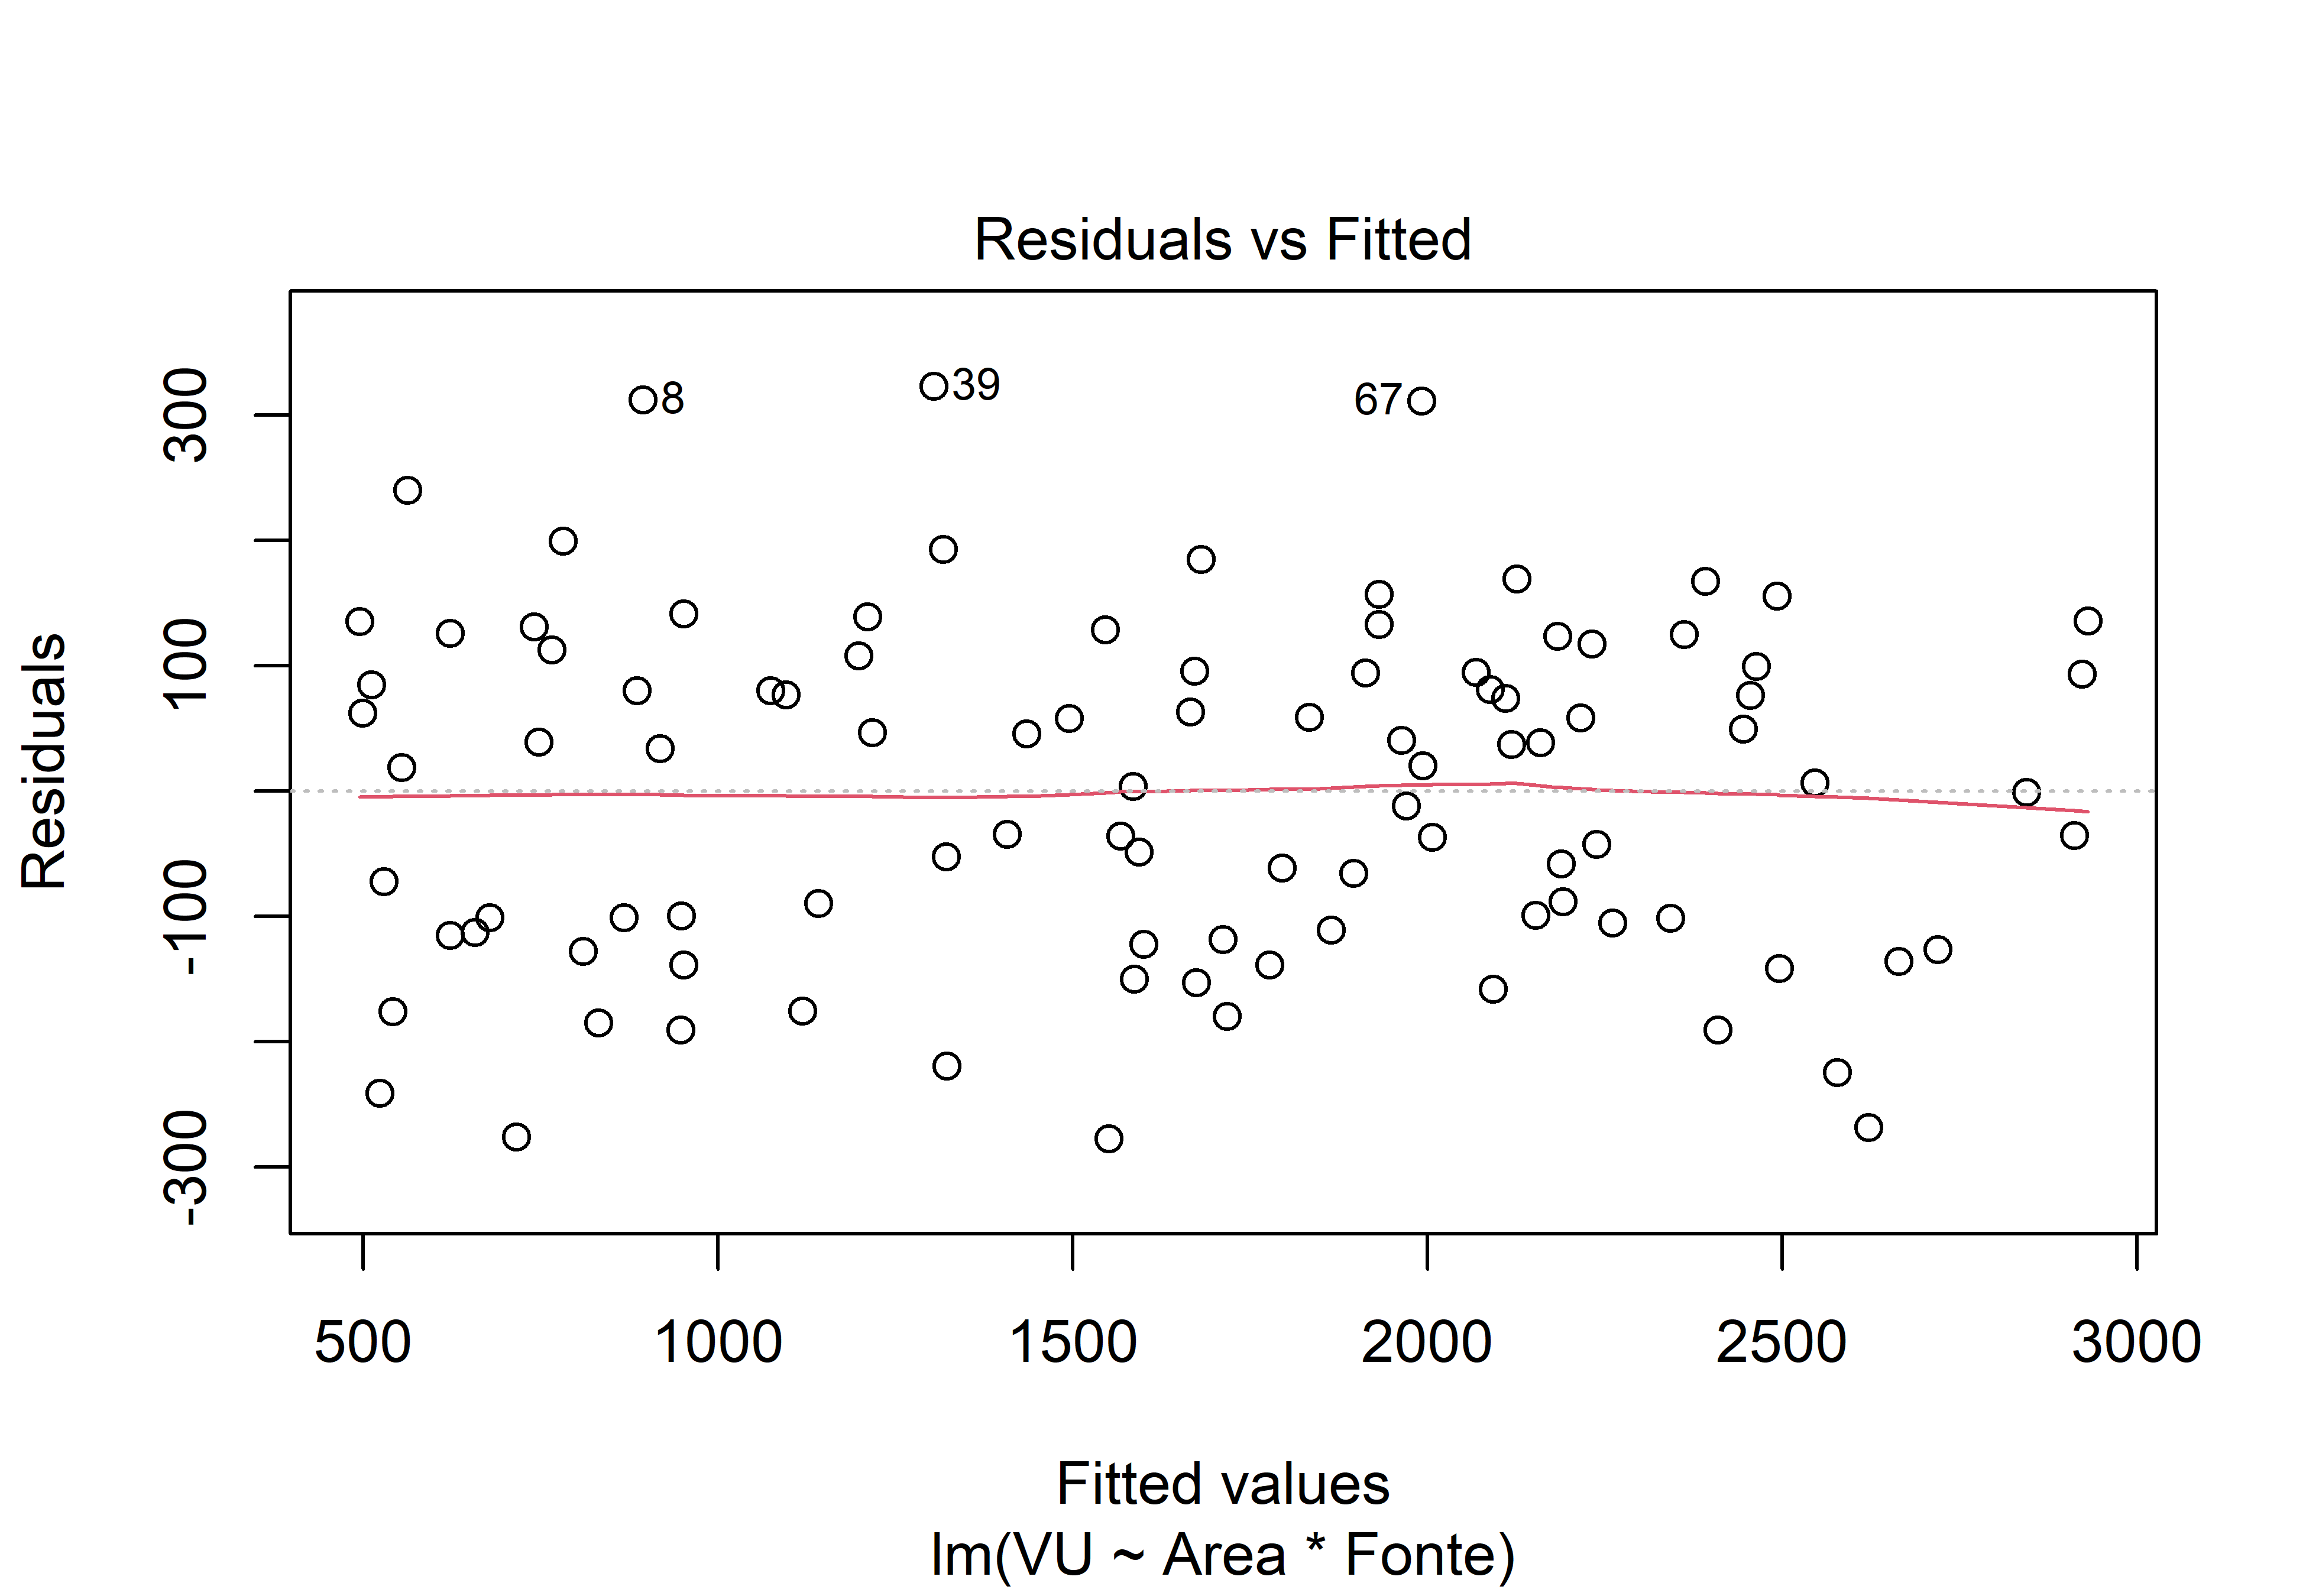
\includegraphics[width=0.5\linewidth]{./images/unnamed-chunk-20-1}
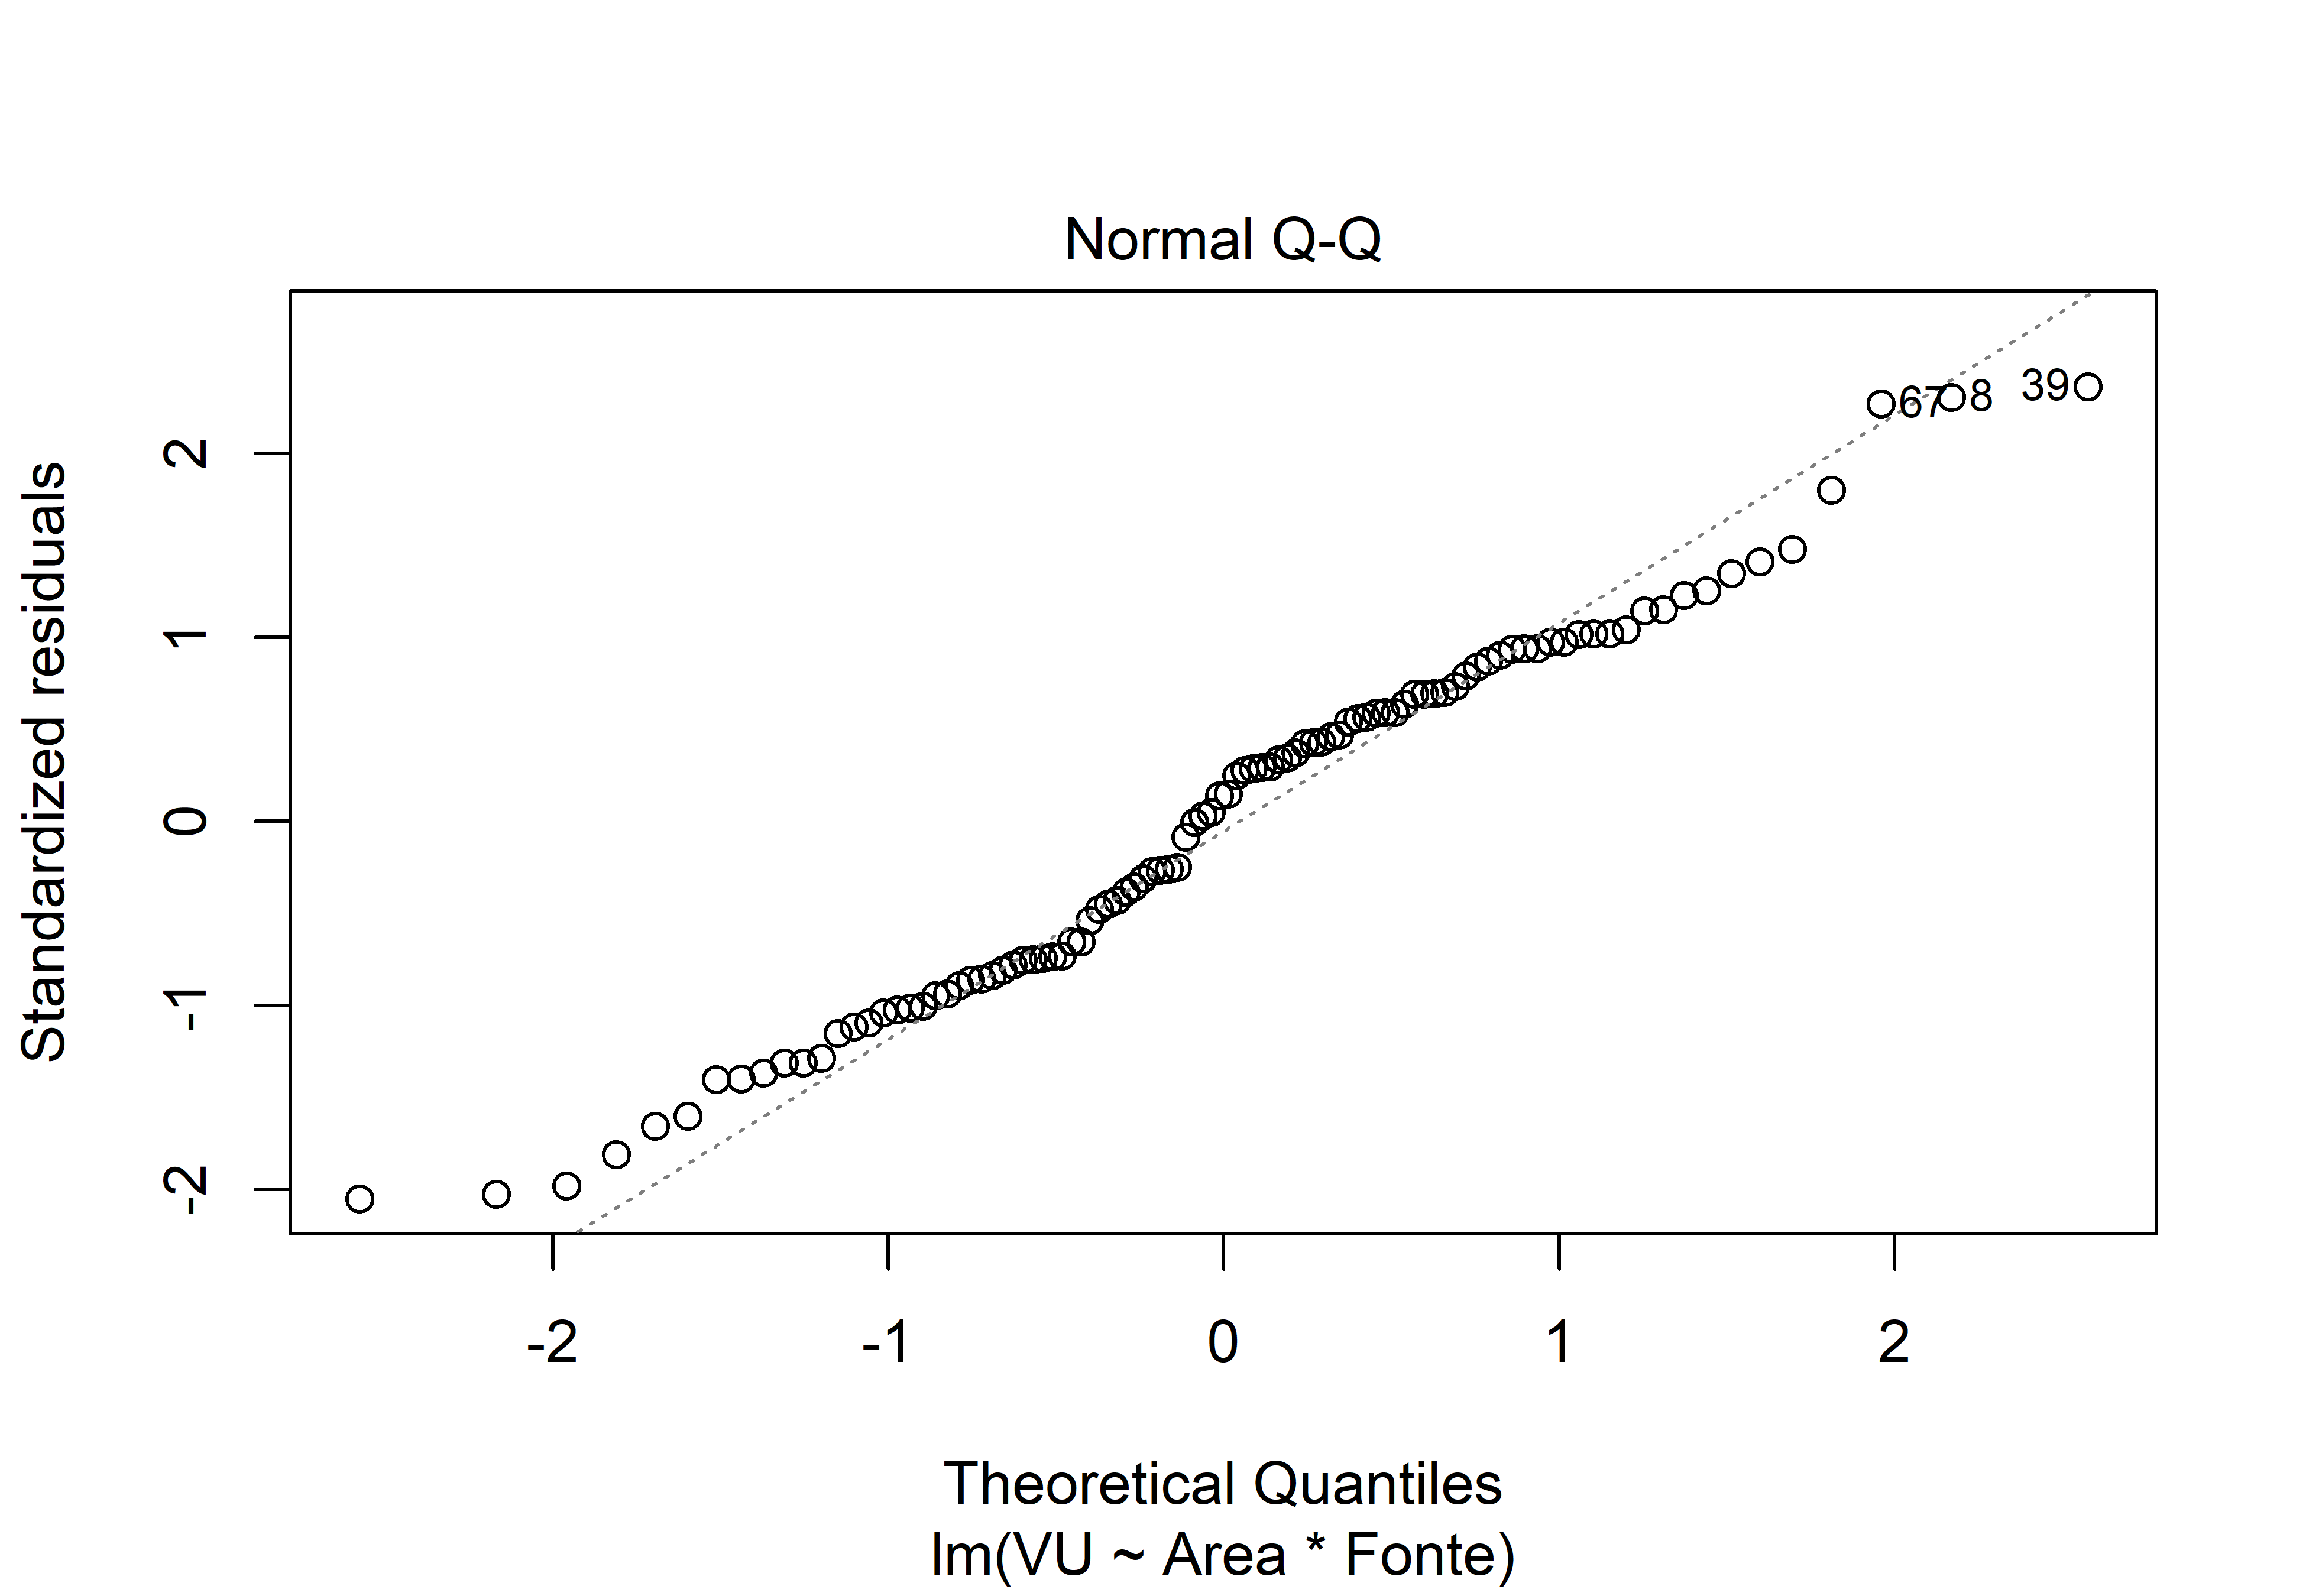
\includegraphics[width=0.5\linewidth]{./images/unnamed-chunk-20-2}
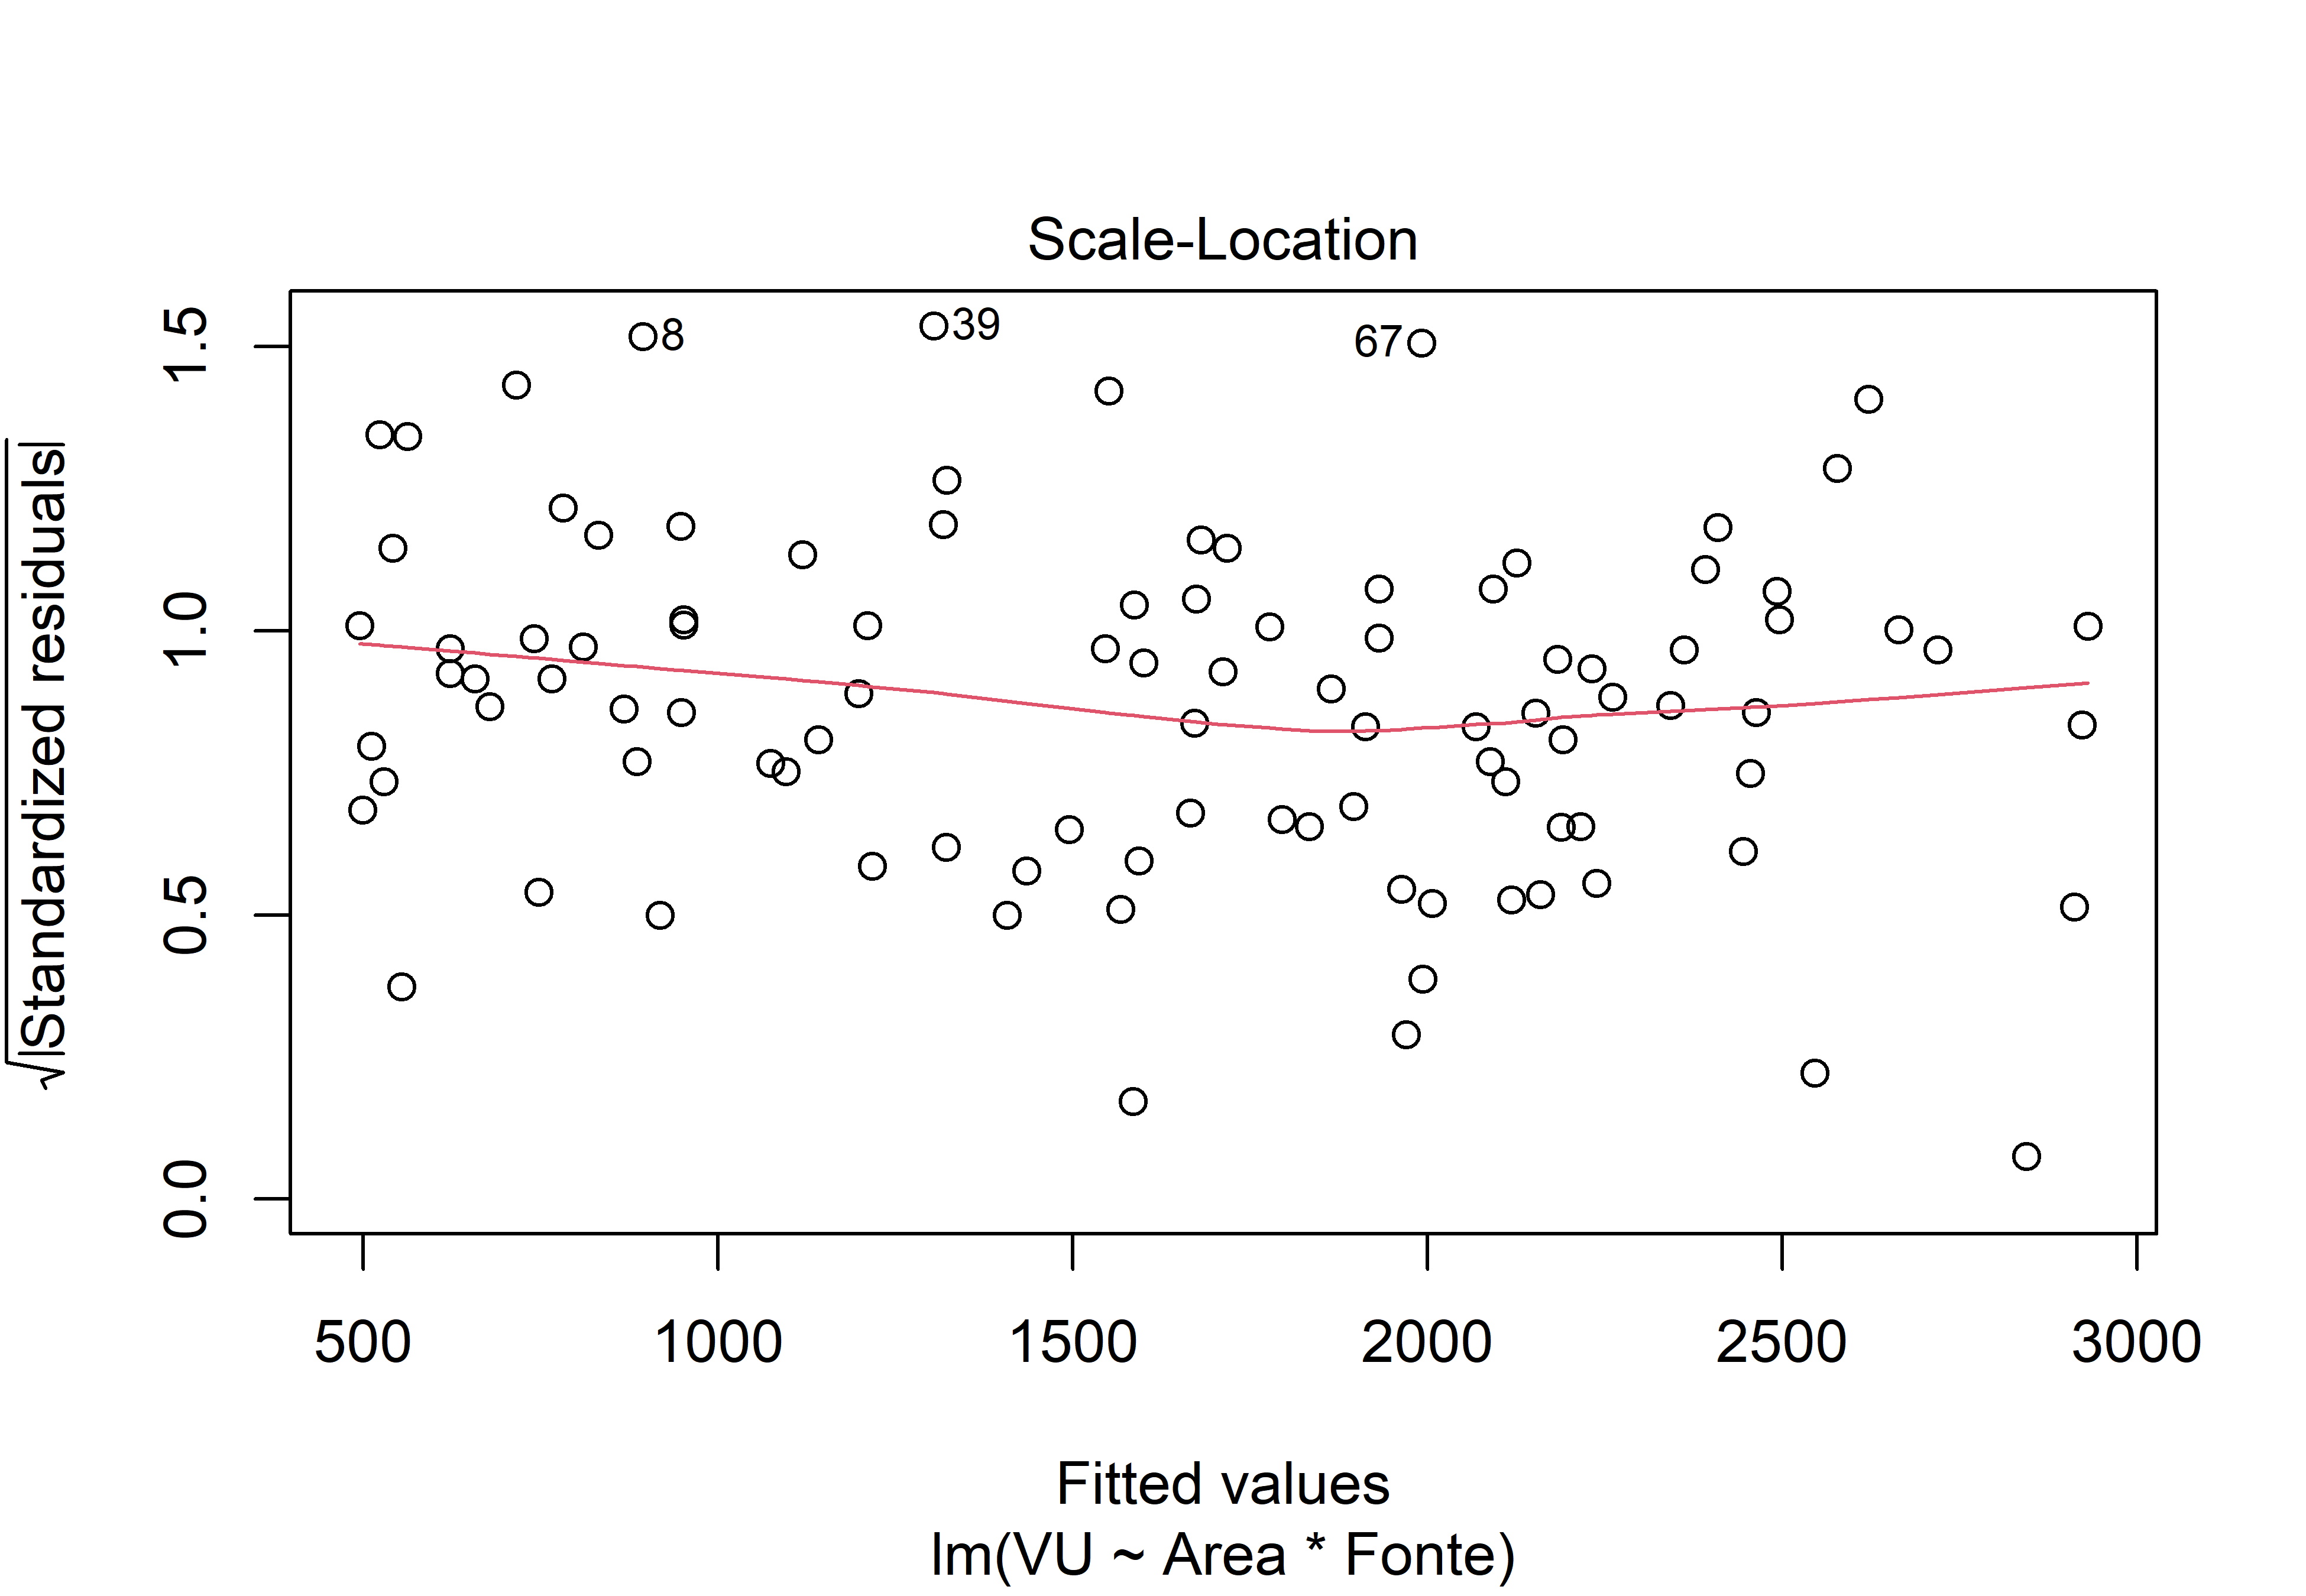
\includegraphics[width=0.5\linewidth]{./images/unnamed-chunk-20-3}
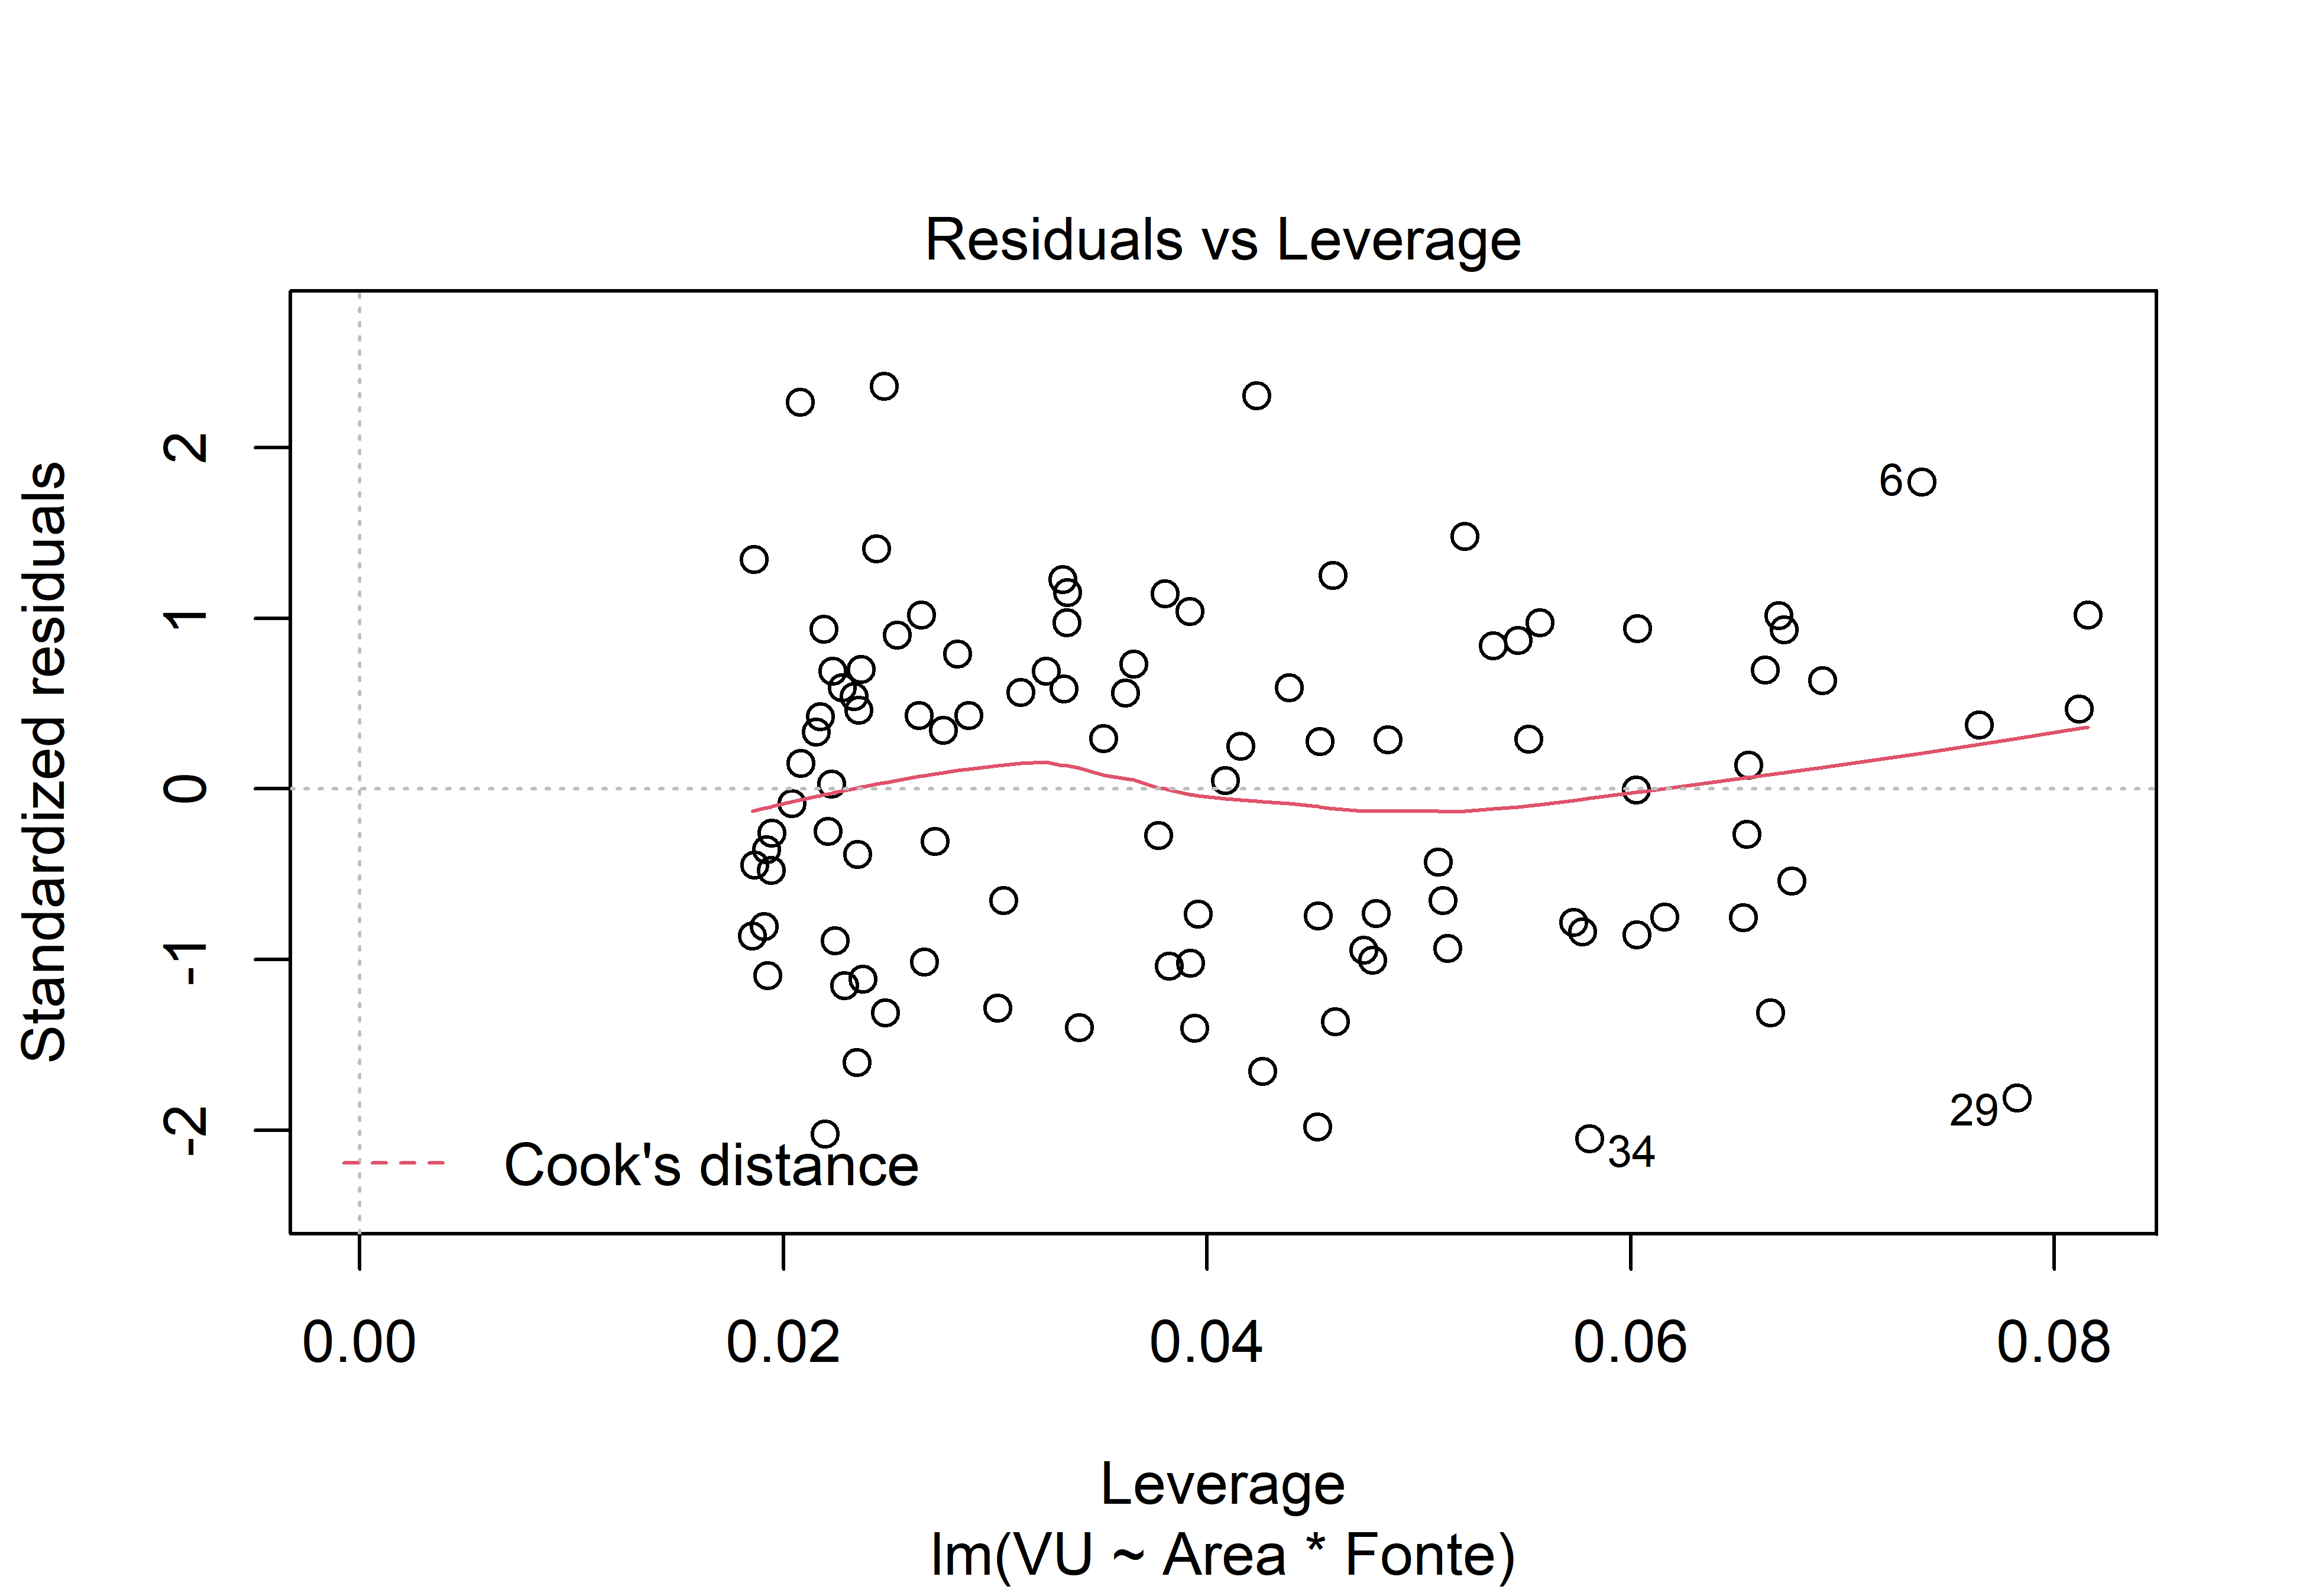
\includegraphics[width=0.5\linewidth]{./images/unnamed-chunk-20-4}

\begin{verbatim}
## 
##  studentized Breusch-Pagan test
## 
## data:  fit1
## BP = 3.9476, df = 3, p-value = 0.2672
\end{verbatim}

Uma opção dada pela ABNT (\protect\hyperlink{ref-NBR1465302}{2011}) é a
prévia homogeneização dos dados, conforme item 9.2.1.3. A Figura
\ref{fig:dadosHomogeneizados} mostra como ficam os dados após a
homogeneização.

\begin{verbatim}
## `geom_smooth()` using formula 'y ~ x'
\end{verbatim}

\begin{figure}
\centering
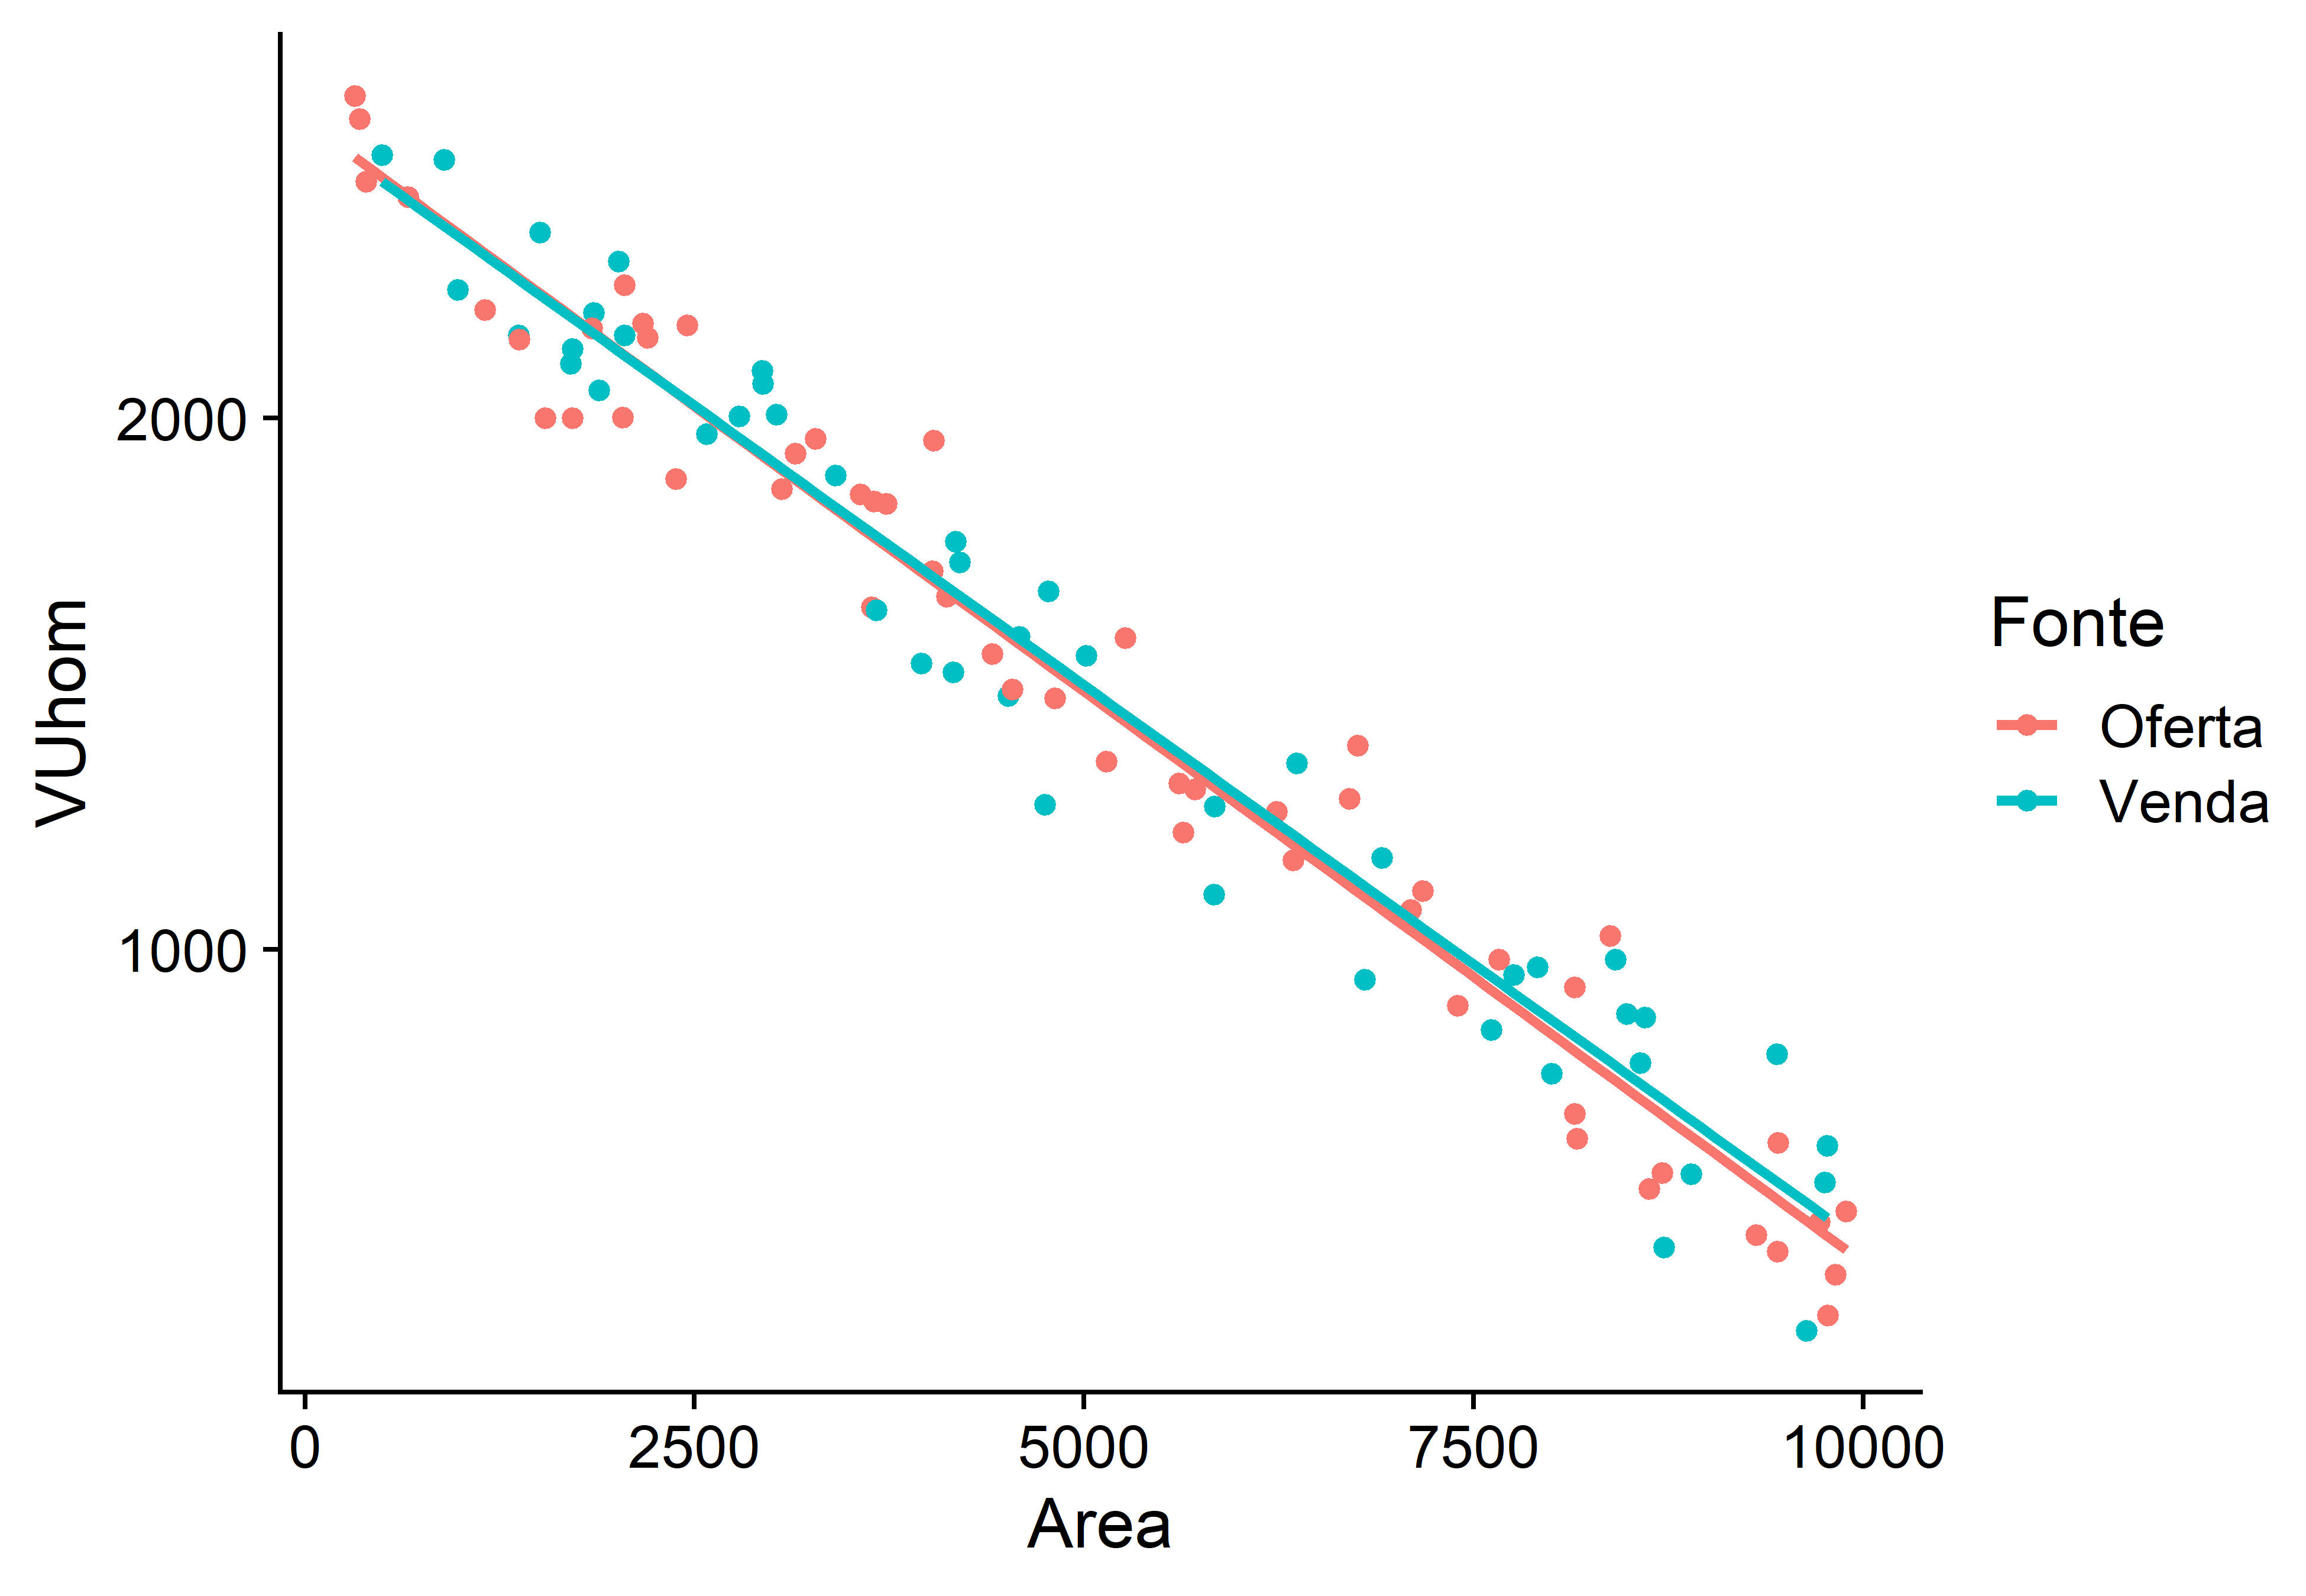
\includegraphics{./images/dadosHomogeneizados-1.png}
\caption{Dados homogeneizados.}
\end{figure}

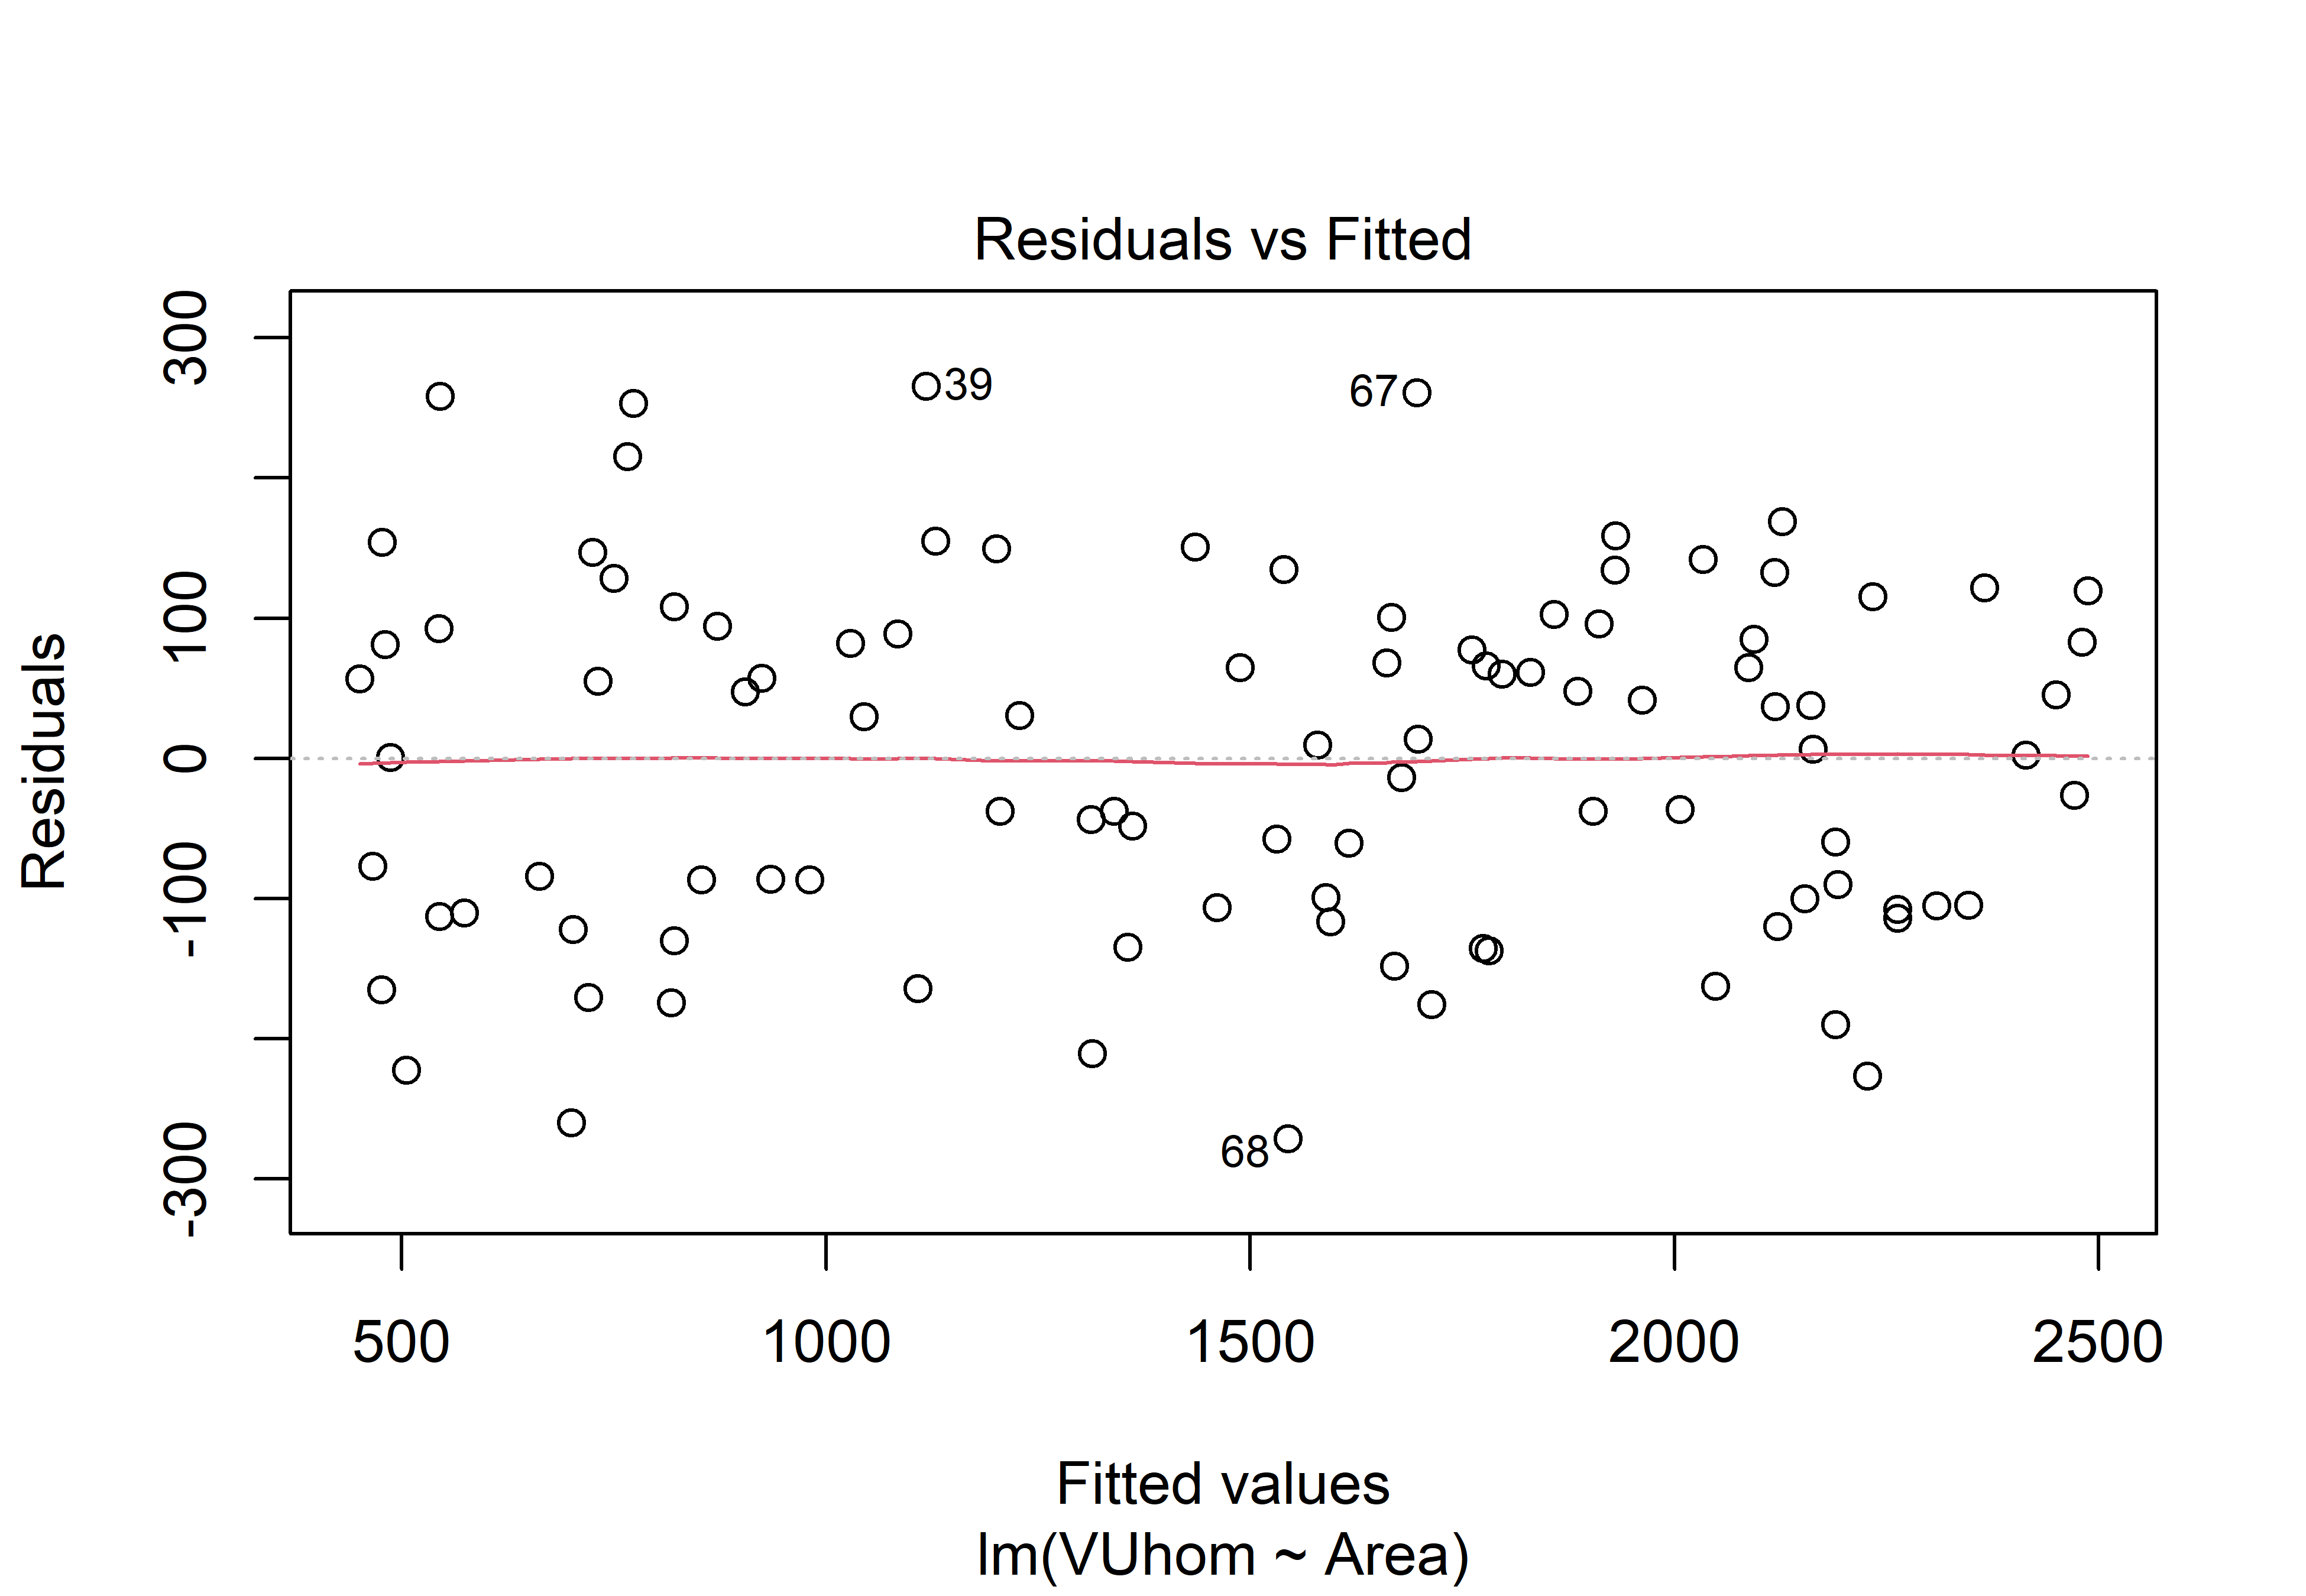
\includegraphics[width=0.5\linewidth]{./images/fithomPlot-1}
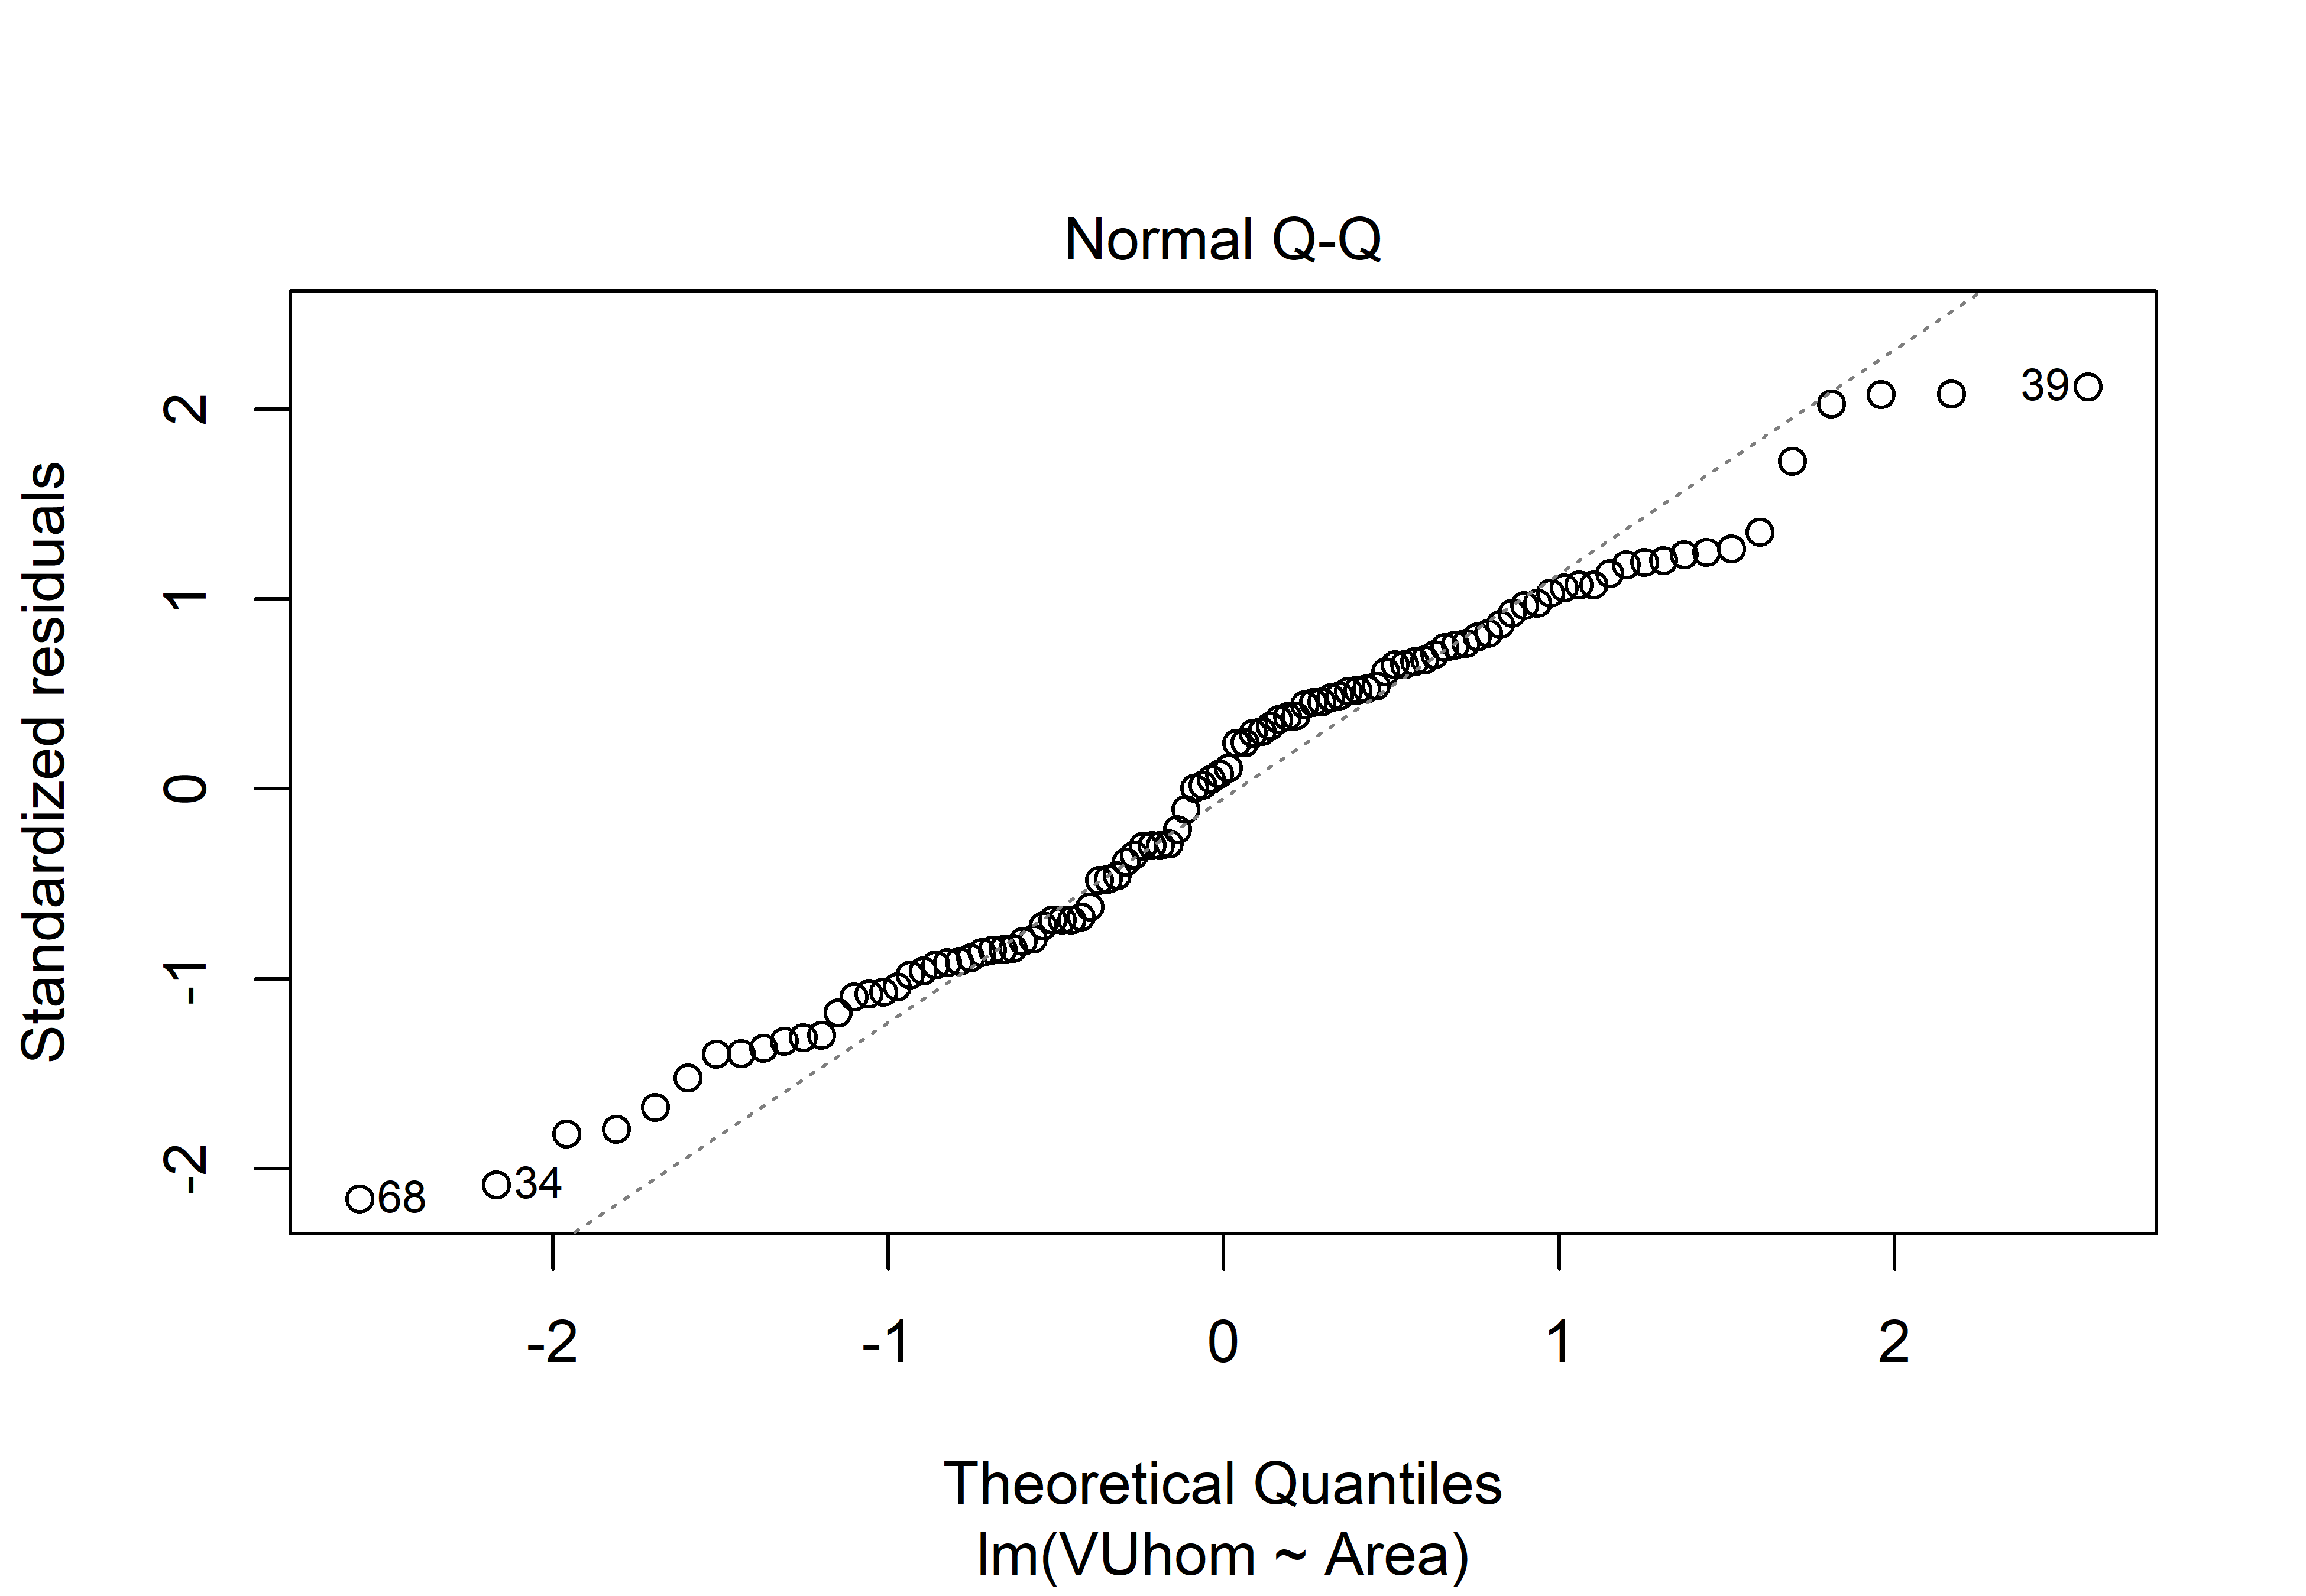
\includegraphics[width=0.5\linewidth]{./images/fithomPlot-2}
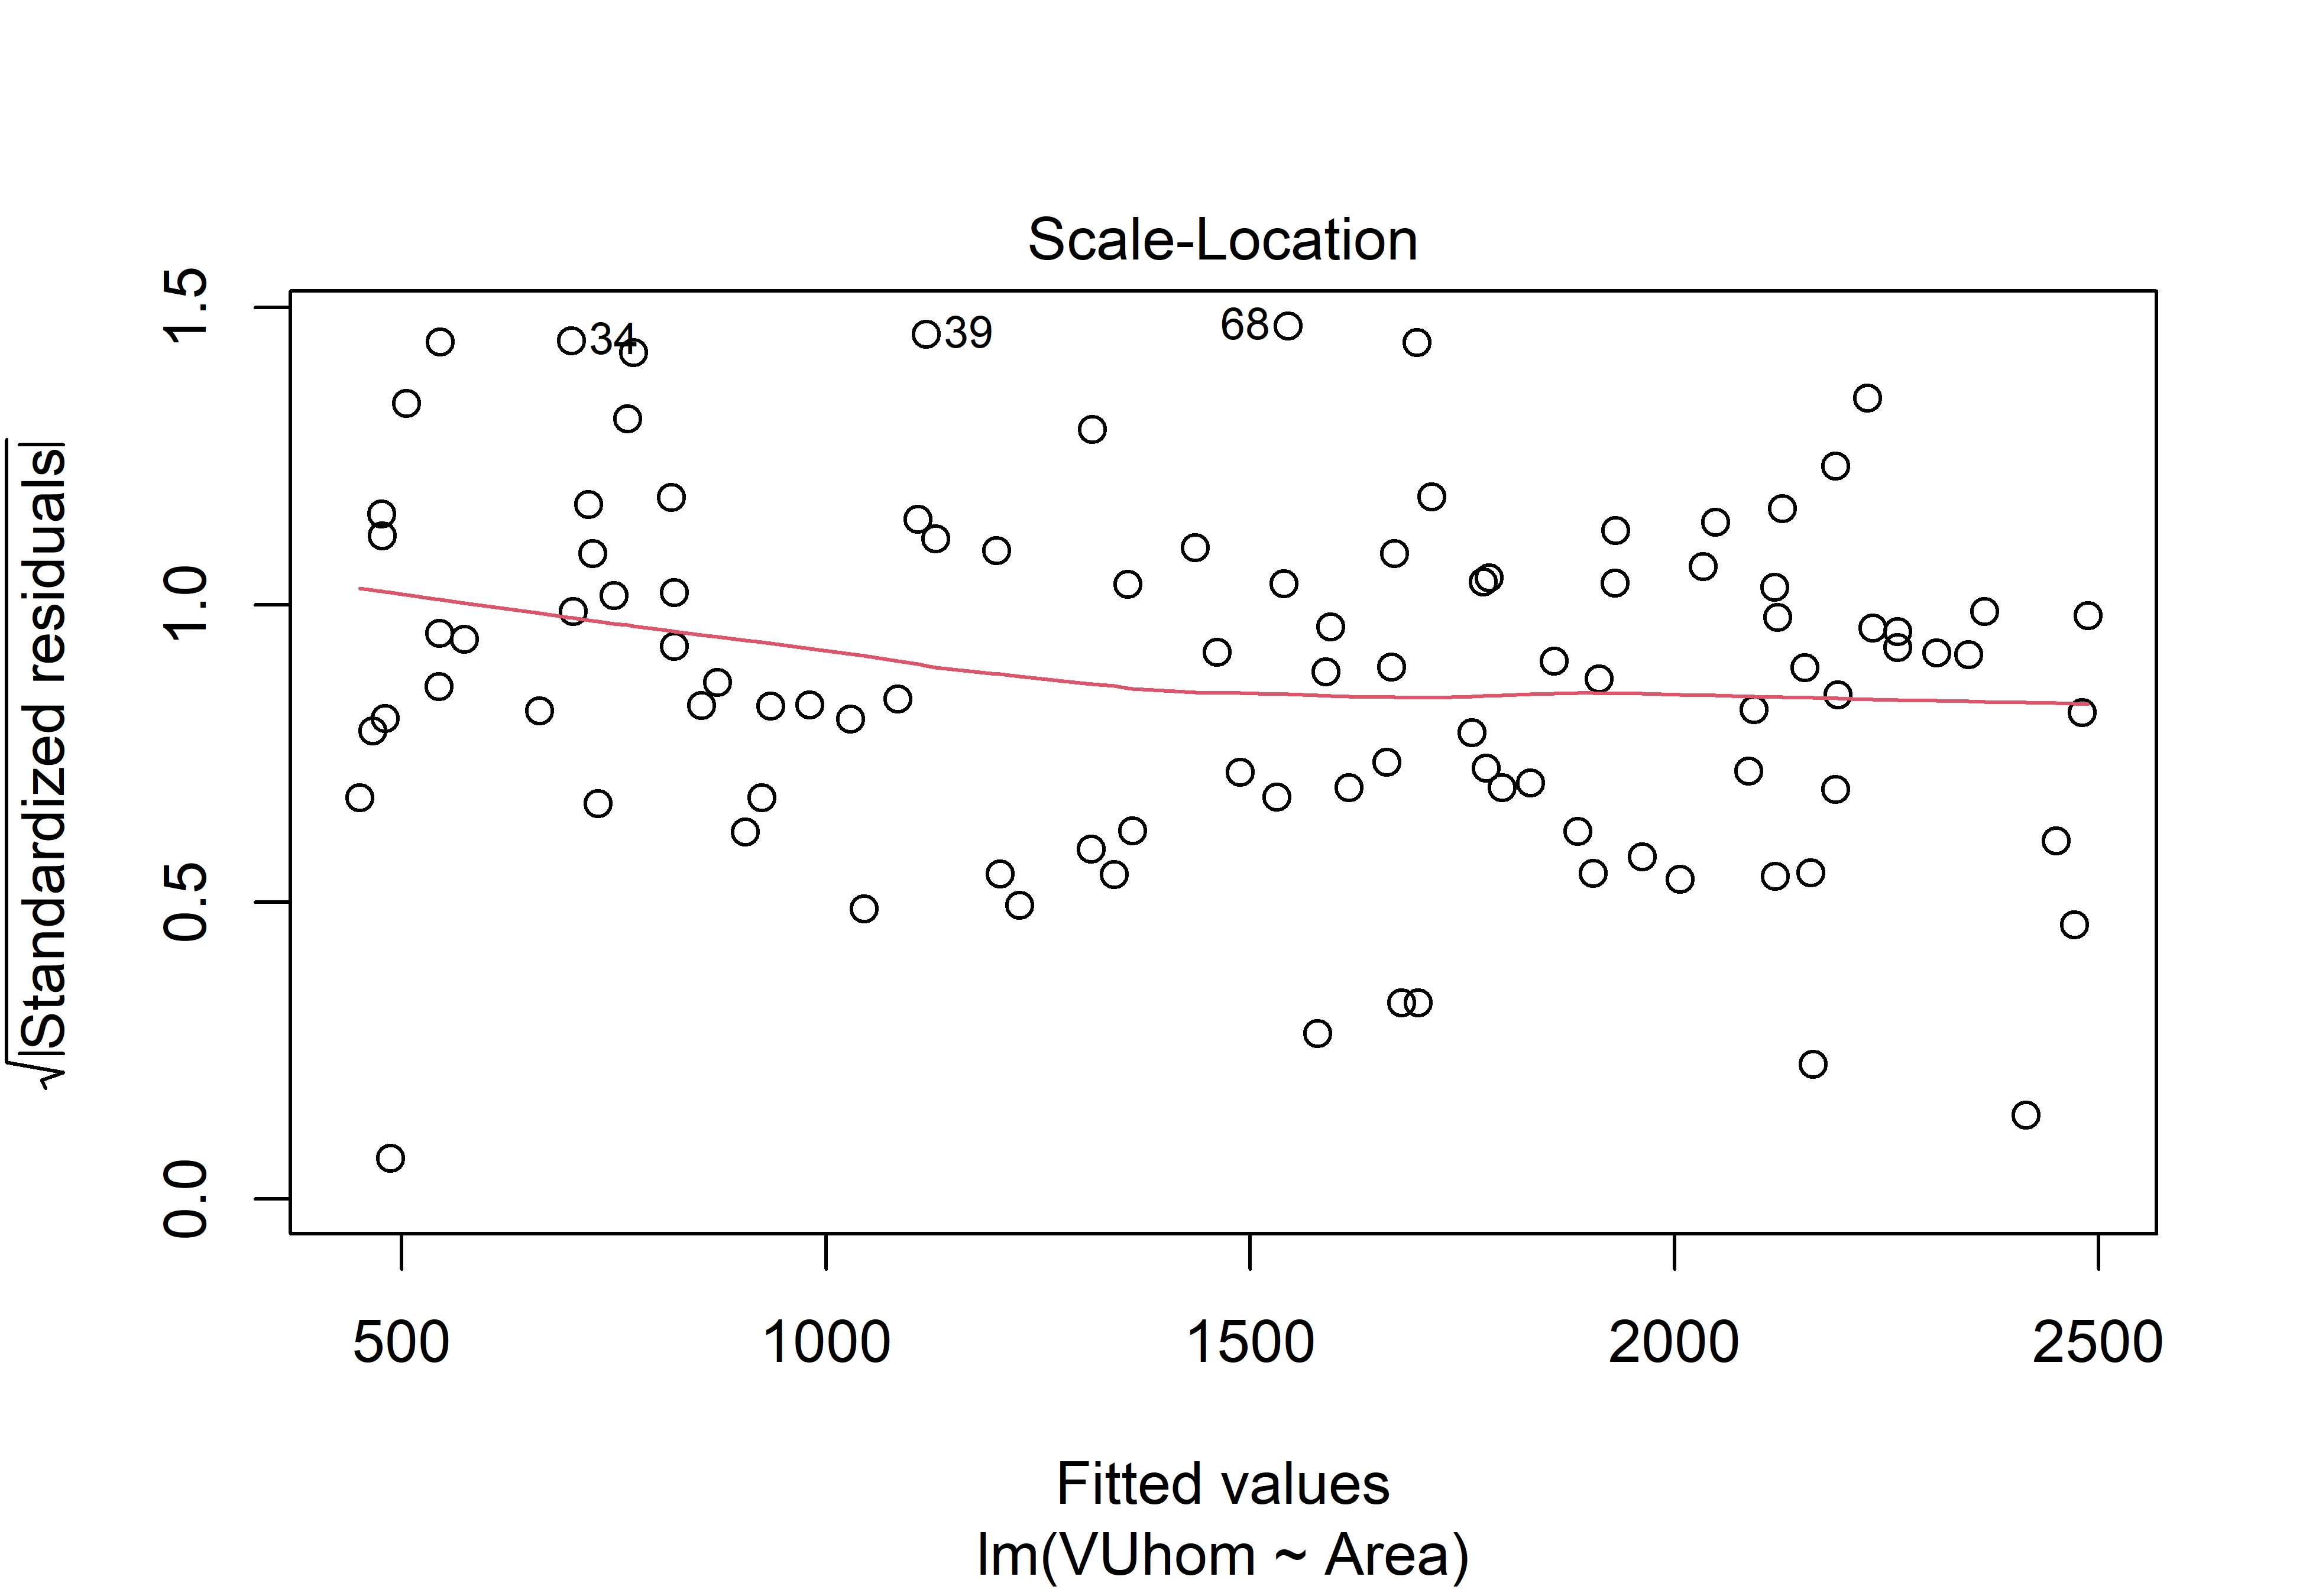
\includegraphics[width=0.5\linewidth]{./images/fithomPlot-3}
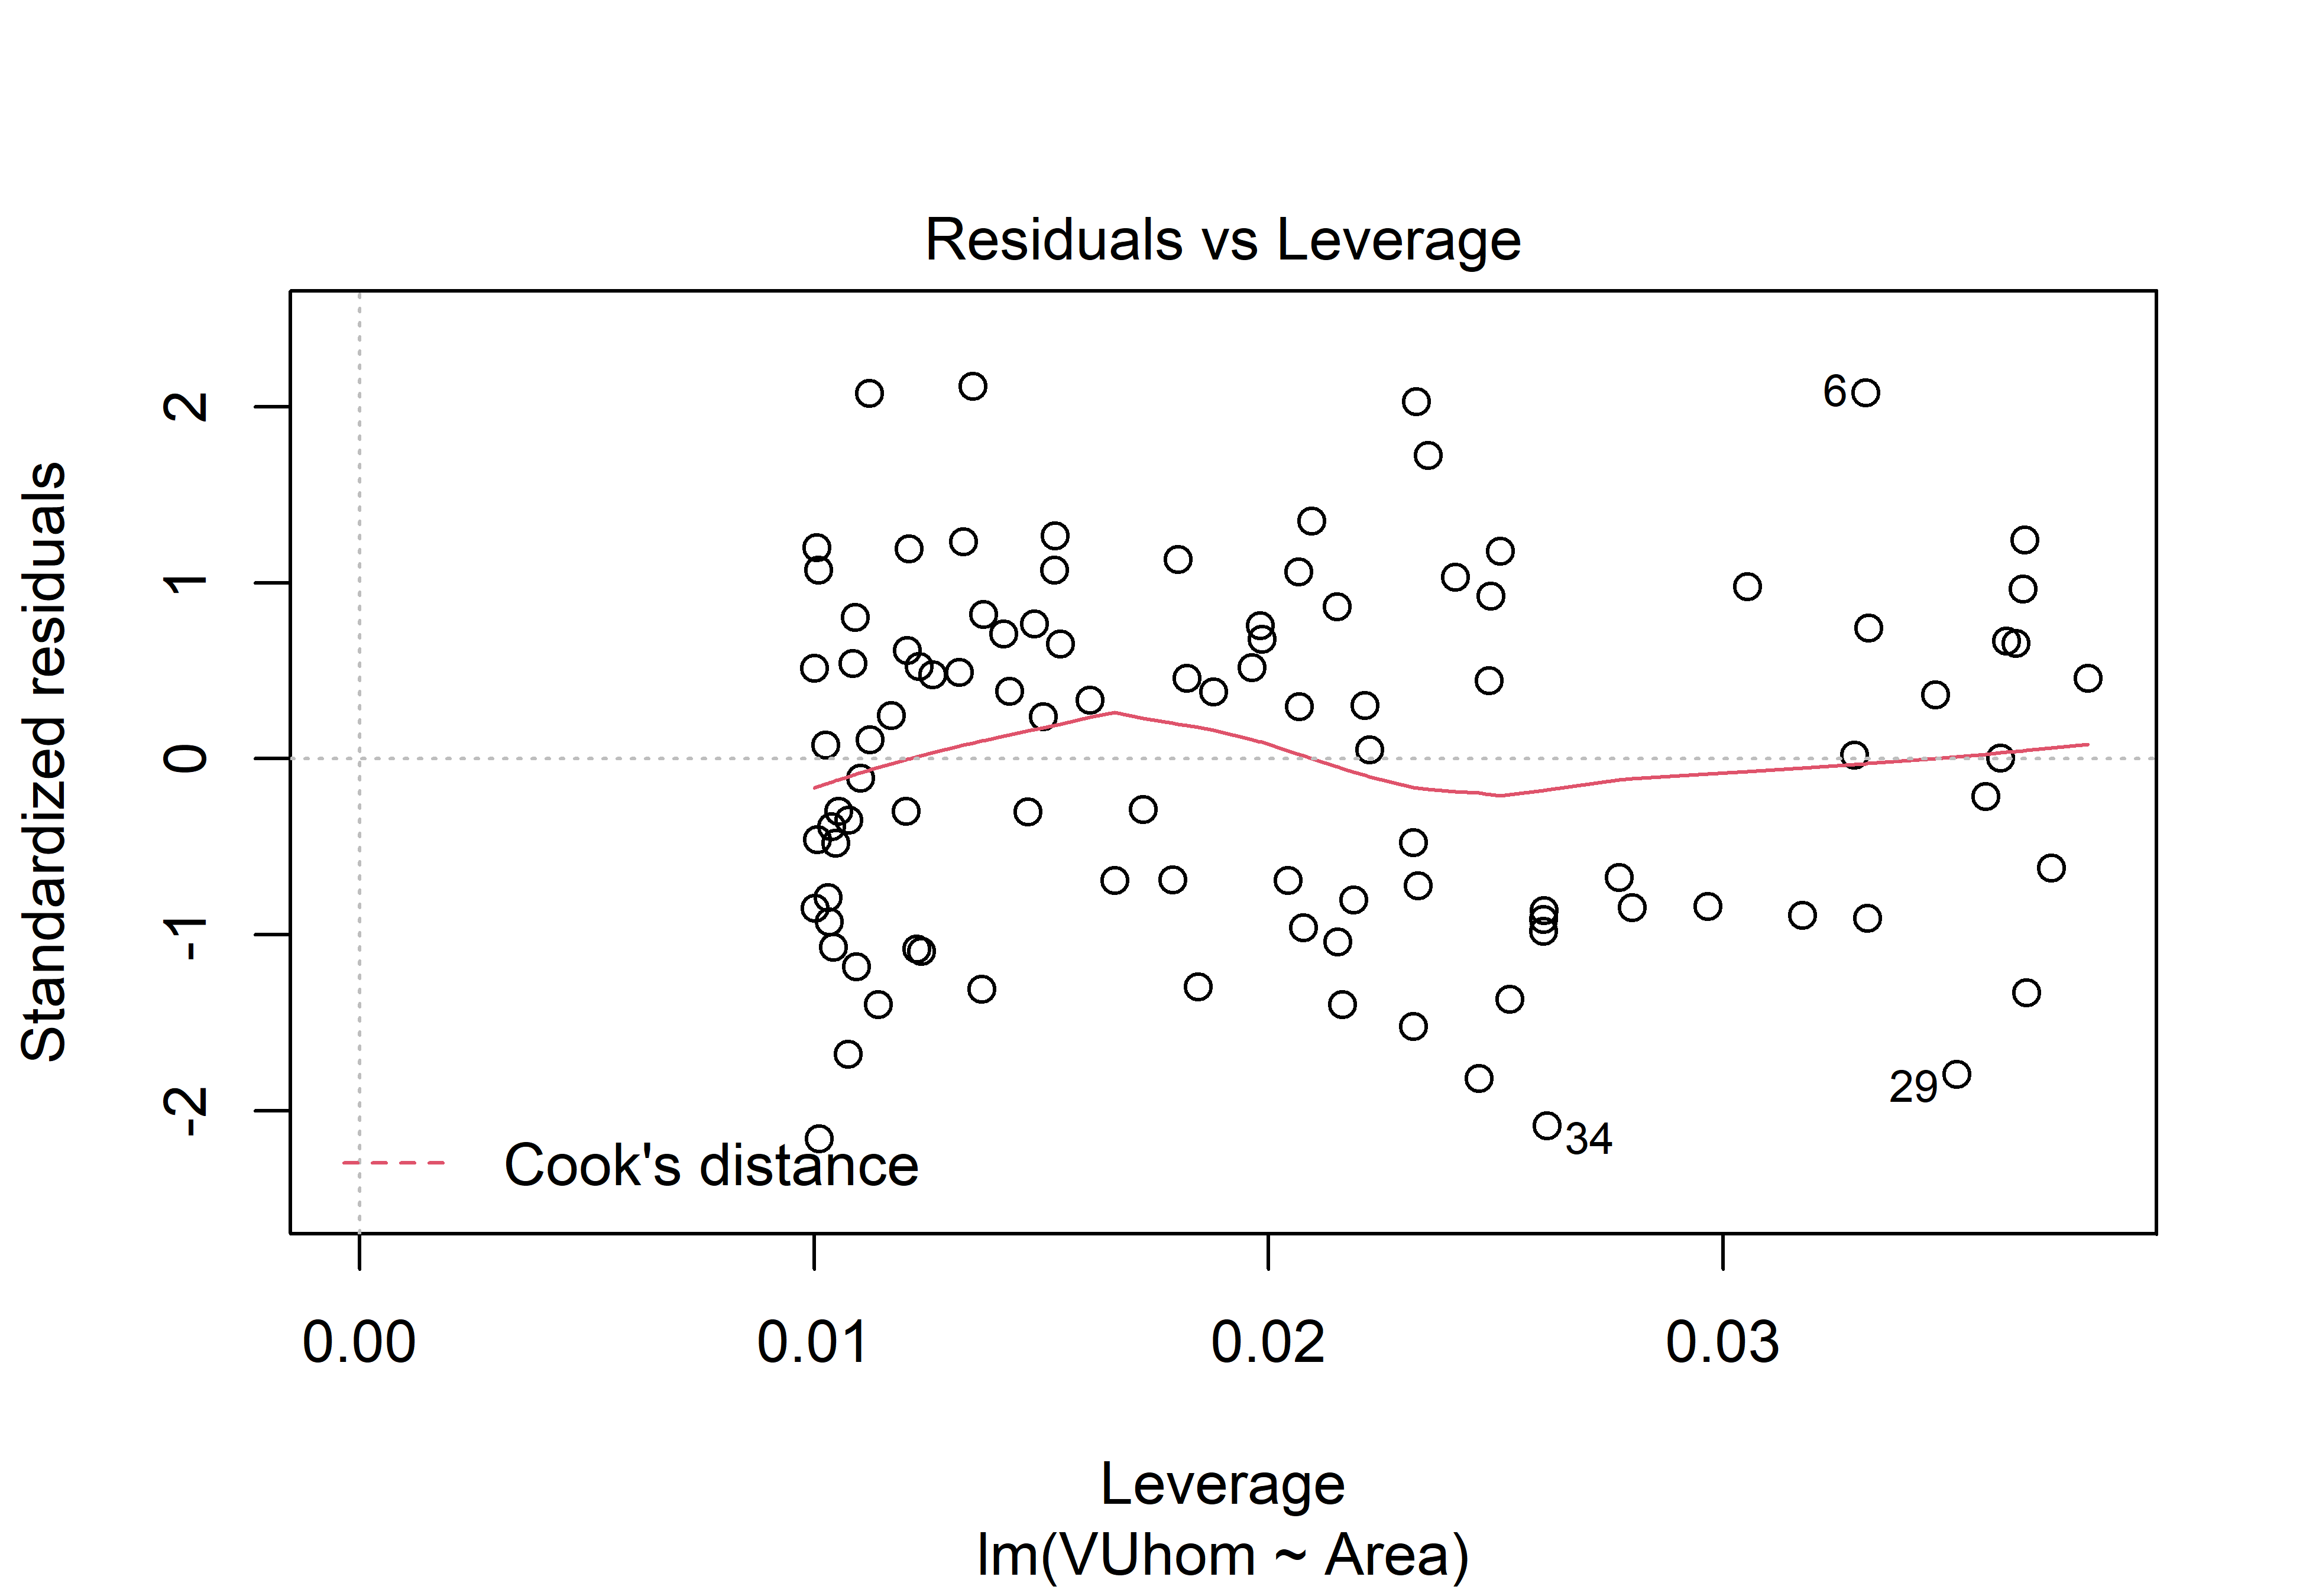
\includegraphics[width=0.5\linewidth]{./images/fithomPlot-4}

\begin{verbatim}
##        1 
## 2550.059
\end{verbatim}

\begin{verbatim}
##        1 
## 2443.899
\end{verbatim}

\begin{verbatim}
##        1 
## 2448.549
\end{verbatim}

\begin{verbatim}
##        1 
## 1498.661
\end{verbatim}

\begin{verbatim}
##        1 
## 1498.004
\end{verbatim}

\begin{verbatim}
##        1 
## 1491.235
\end{verbatim}

\begin{verbatim}
##        1 
## 330.4401
\end{verbatim}

\begin{verbatim}
##        1 
## 447.0103
\end{verbatim}

\begin{verbatim}
##        1 
## 427.5531
\end{verbatim}

\begin{table}[H] \centering 
  \caption{Comparação dos modelos} 
  \label{} 
\begin{tabular}{@{\extracolsep{5pt}}lccc} 
\\[-1.8ex]\hline 
\hline \\[-1.8ex] 
 & \multicolumn{3}{c}{\textit{Dependent variable:}} \\ 
\cline{2-4} 
\\[-1.8ex] & \multicolumn{2}{c}{VU} & VUhom \\ 
\\[-1.8ex] & (1) & (2) & (3)\\ 
\hline \\[-1.8ex] 
 Constant & 2.914,83 (2.871,91, 2.957,75) & 3.011,07 (2.962,81, 3.059,33) & 2.554,92 (2.522,42, 2.587,41) \\ 
  & t = 87,04$^{***}$ & t = 79,96$^{***}$ & t = 100,76$^{***}$ \\ 
  Area & $-$0,23 ($-$0,24, $-$0,23) & $-$0,25 ($-$0,26, $-$0,24) & $-$0,21 ($-$0,22, $-$0,21) \\ 
  & t = $-$44,72$^{***}$ & t = $-$39,20$^{***}$ & t = $-$48,79$^{***}$ \\ 
  FonteVenda & $-$247,95 ($-$286,85, $-$209,04) & $-$462,07 ($-$533,77, $-$390,38) &  \\ 
  & t = $-$8,17$^{***}$ & t = $-$8,26$^{***}$ &  \\ 
  Area:FonteVenda &  & 0,04 (0,03, 0,05) &  \\ 
  &  & t = 4,41$^{***}$ &  \\ 
 \hline \\[-1.8ex] 
Observations & 100 & 100 & 100 \\ 
R$^{2}$ & 0,96 & 0,96 & 0,96 \\ 
Adjusted R$^{2}$ & 0,95 & 0,96 & 0,96 \\ 
Residual Std. Error & 151,29 (df = 97) & 138,67 (df = 96) & 126,27 (df = 98) \\ 
F Statistic & 1.031,74$^{***}$ (df = 2; 97) & 825,26$^{***}$ (df = 3; 96) & 2.380,72$^{***}$ (df = 1; 98) \\ 
\hline 
\hline \\[-1.8ex] 
Notas: & \multicolumn{3}{r}{$^{*}$p$<$0,3; $^{**}$p$<$0,2; $^{***}$p$<$0,1} \\ 
\end{tabular} 
\end{table}

\hypertarget{ec3}{%
\subsection{EC3}\label{ec3}}

Outra possibilidade é o ajuste do modelo com a transformação da variável
dependente para a escala logarítmica, o que é muito comum na Engenharia
de Avaliações. A transformação, porém, não deve ser feita em função
apenas da modelagem do fator oferta: uma vez averiguada a necessidade de
transformação da variável dependente para a escala logarítmica, pode-se
simplesmente adicionar a variável \(Fonte\) ao lado direto da equação de
regressão, sem a necessidade da adição de termos de interação\footnote{Isto
  decorre do fato que a equação de regressão na forma logarítmica, a
  equação de estimação, obtida pela retransformação da equação de
  regressão para a forma direta, através utilização da função
  exponencial, relaciona os termos de uma maneira multiplicativa. Por
  exemplo: se a regressão for ajustada com a forma
  \(log(Y) \sim \beta_1 X_1 + \beta_2 X_2 + \varepsilon\), então a
  equação de estimação será
  \(Y = \exp(\beta_1 X_1 + \beta_2 X_2) = \exp(\beta_1 X_1)\cdot \exp(\beta_2 X_2)\).}.

Foram gerados, então, 100 dados de oferta/transações através da seguinte
expressão, com \(\varepsilon \sim N(0, .05^2)\):

\[VU = \exp(7,5 - 0,25\cdot \log(Area) - 0,15\cdot Fonte + \varepsilon)\]

\begin{verbatim}
## `geom_smooth()` using method = 'loess' and formula 'y ~ x'
\end{verbatim}

\begin{verbatim}
## `geom_smooth()` using formula 'y ~ x'
\end{verbatim}

\begin{verbatim}
## `geom_smooth()` using method = 'loess' and formula 'y ~ x'
\end{verbatim}

\begin{figure}
\centering
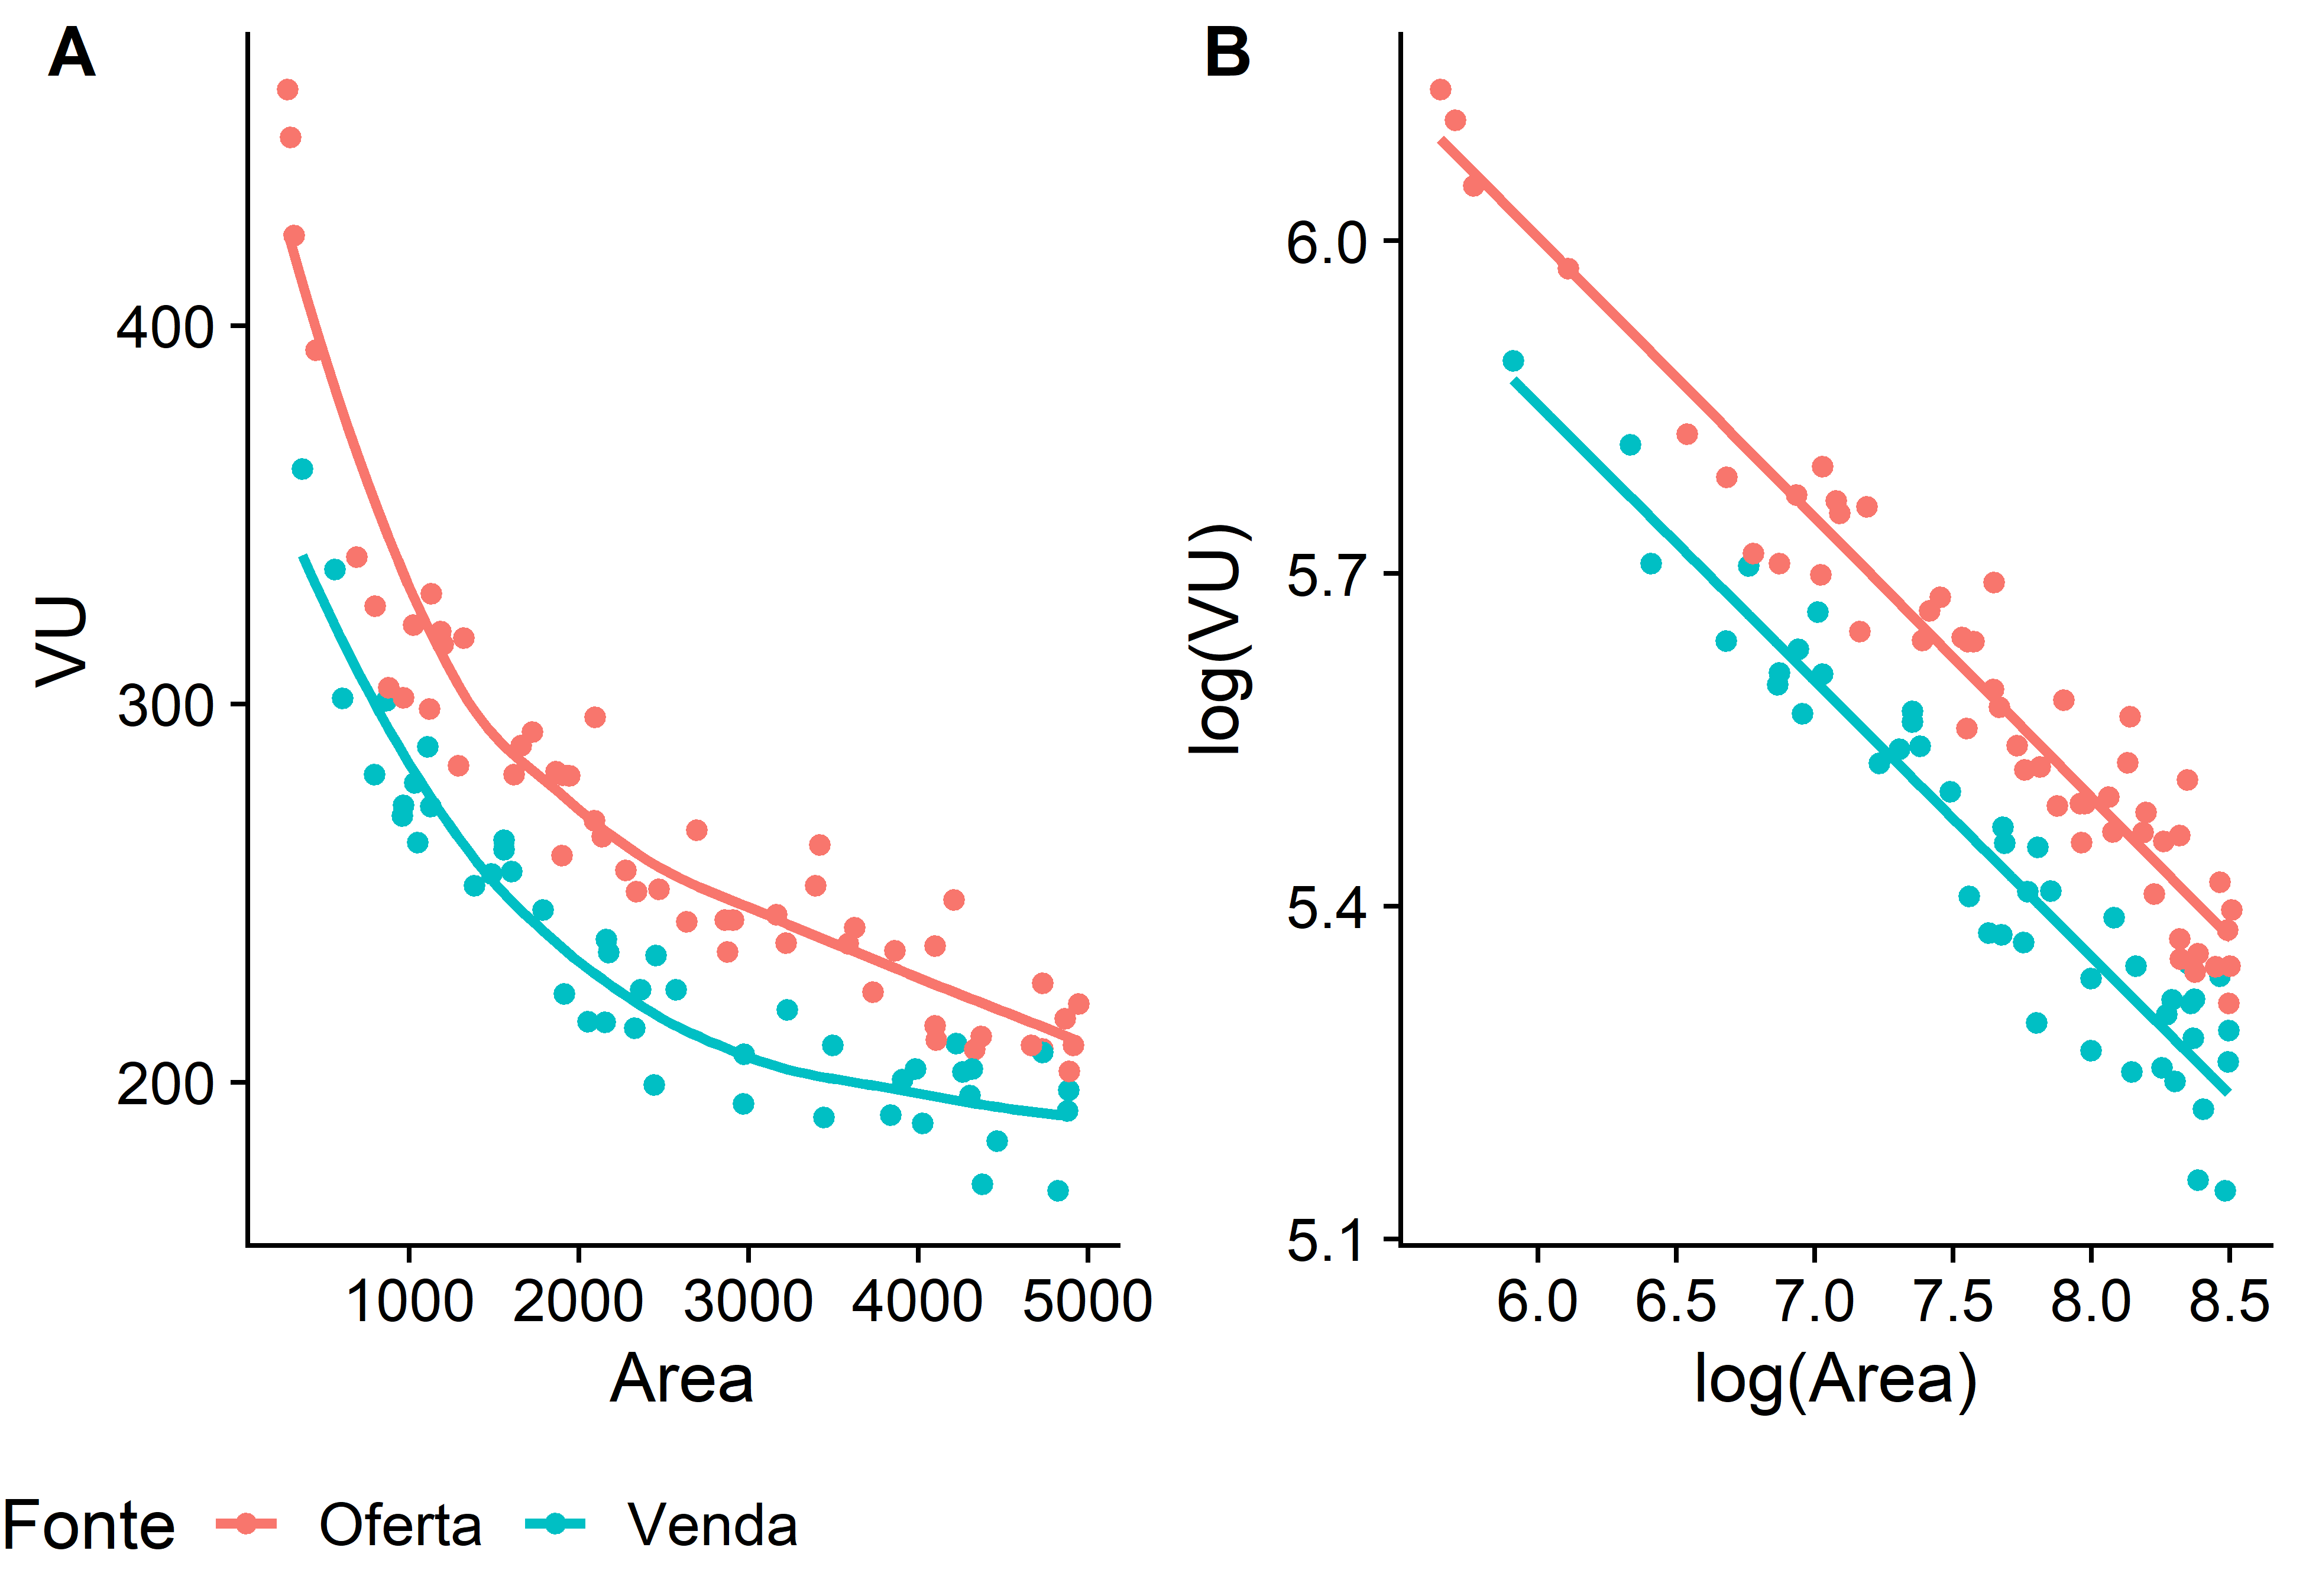
\includegraphics{./images/dados2-1.png}
\caption{Dados com distribuição lognormal.}
\end{figure}

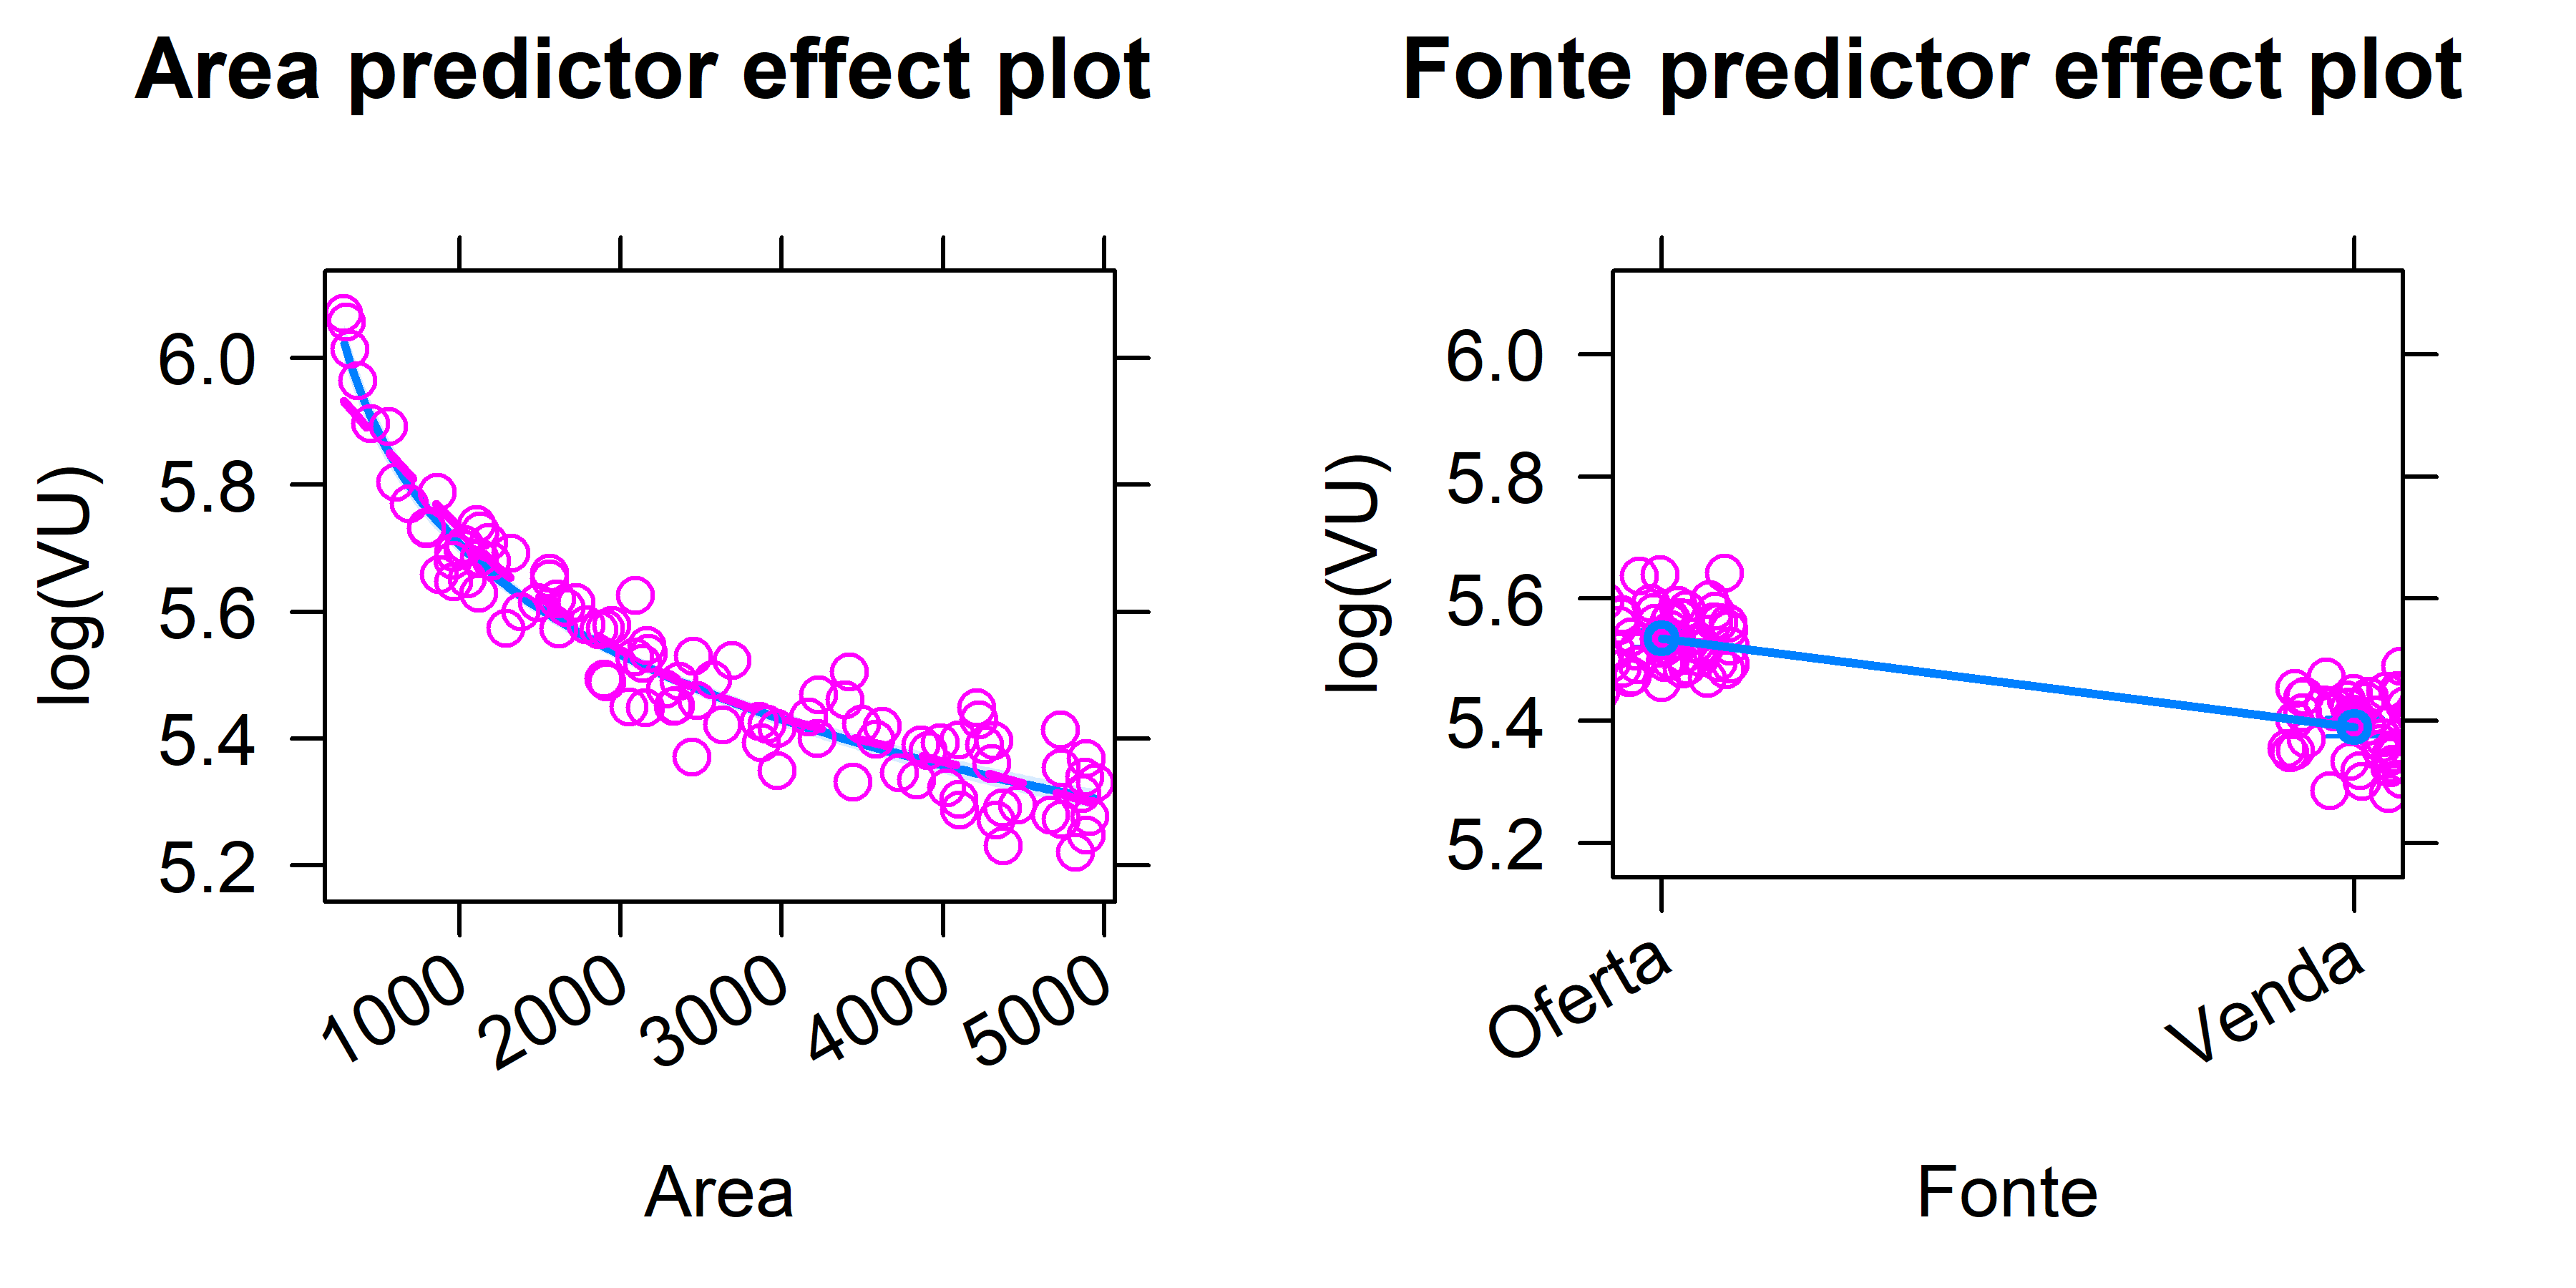
\includegraphics{./images/unnamed-chunk-27-1.png}

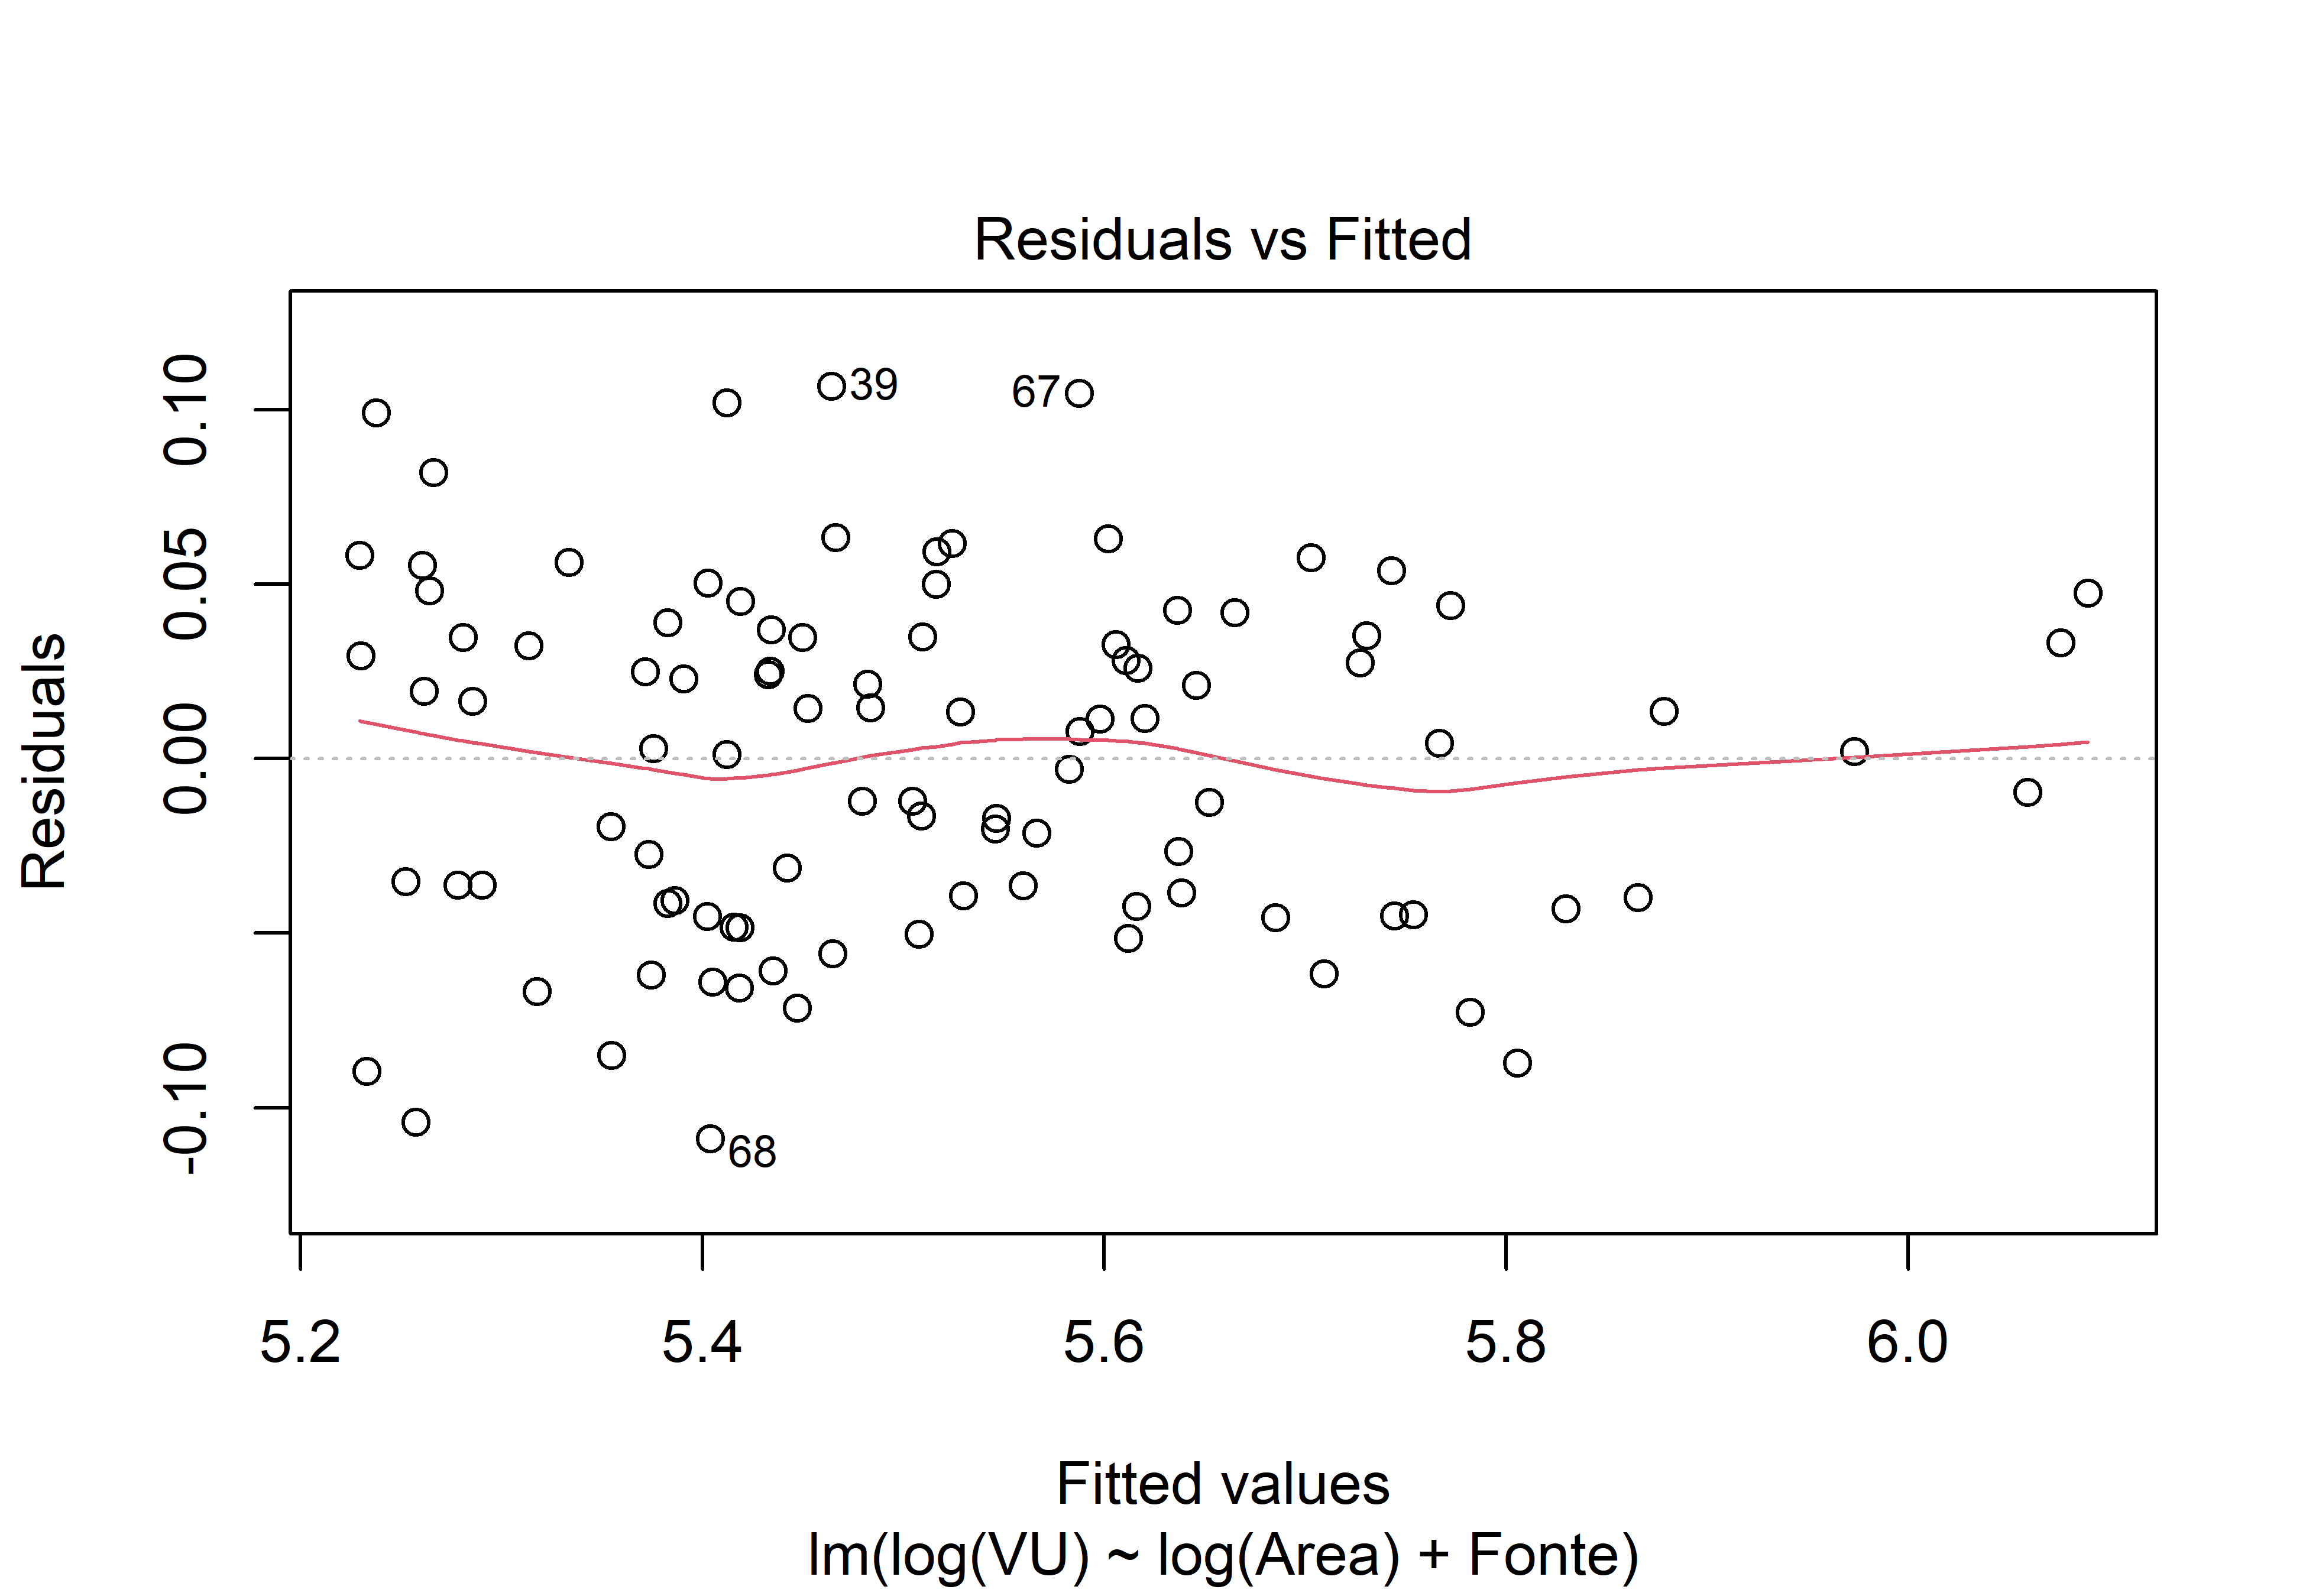
\includegraphics[width=0.5\linewidth]{./images/unnamed-chunk-28-1}
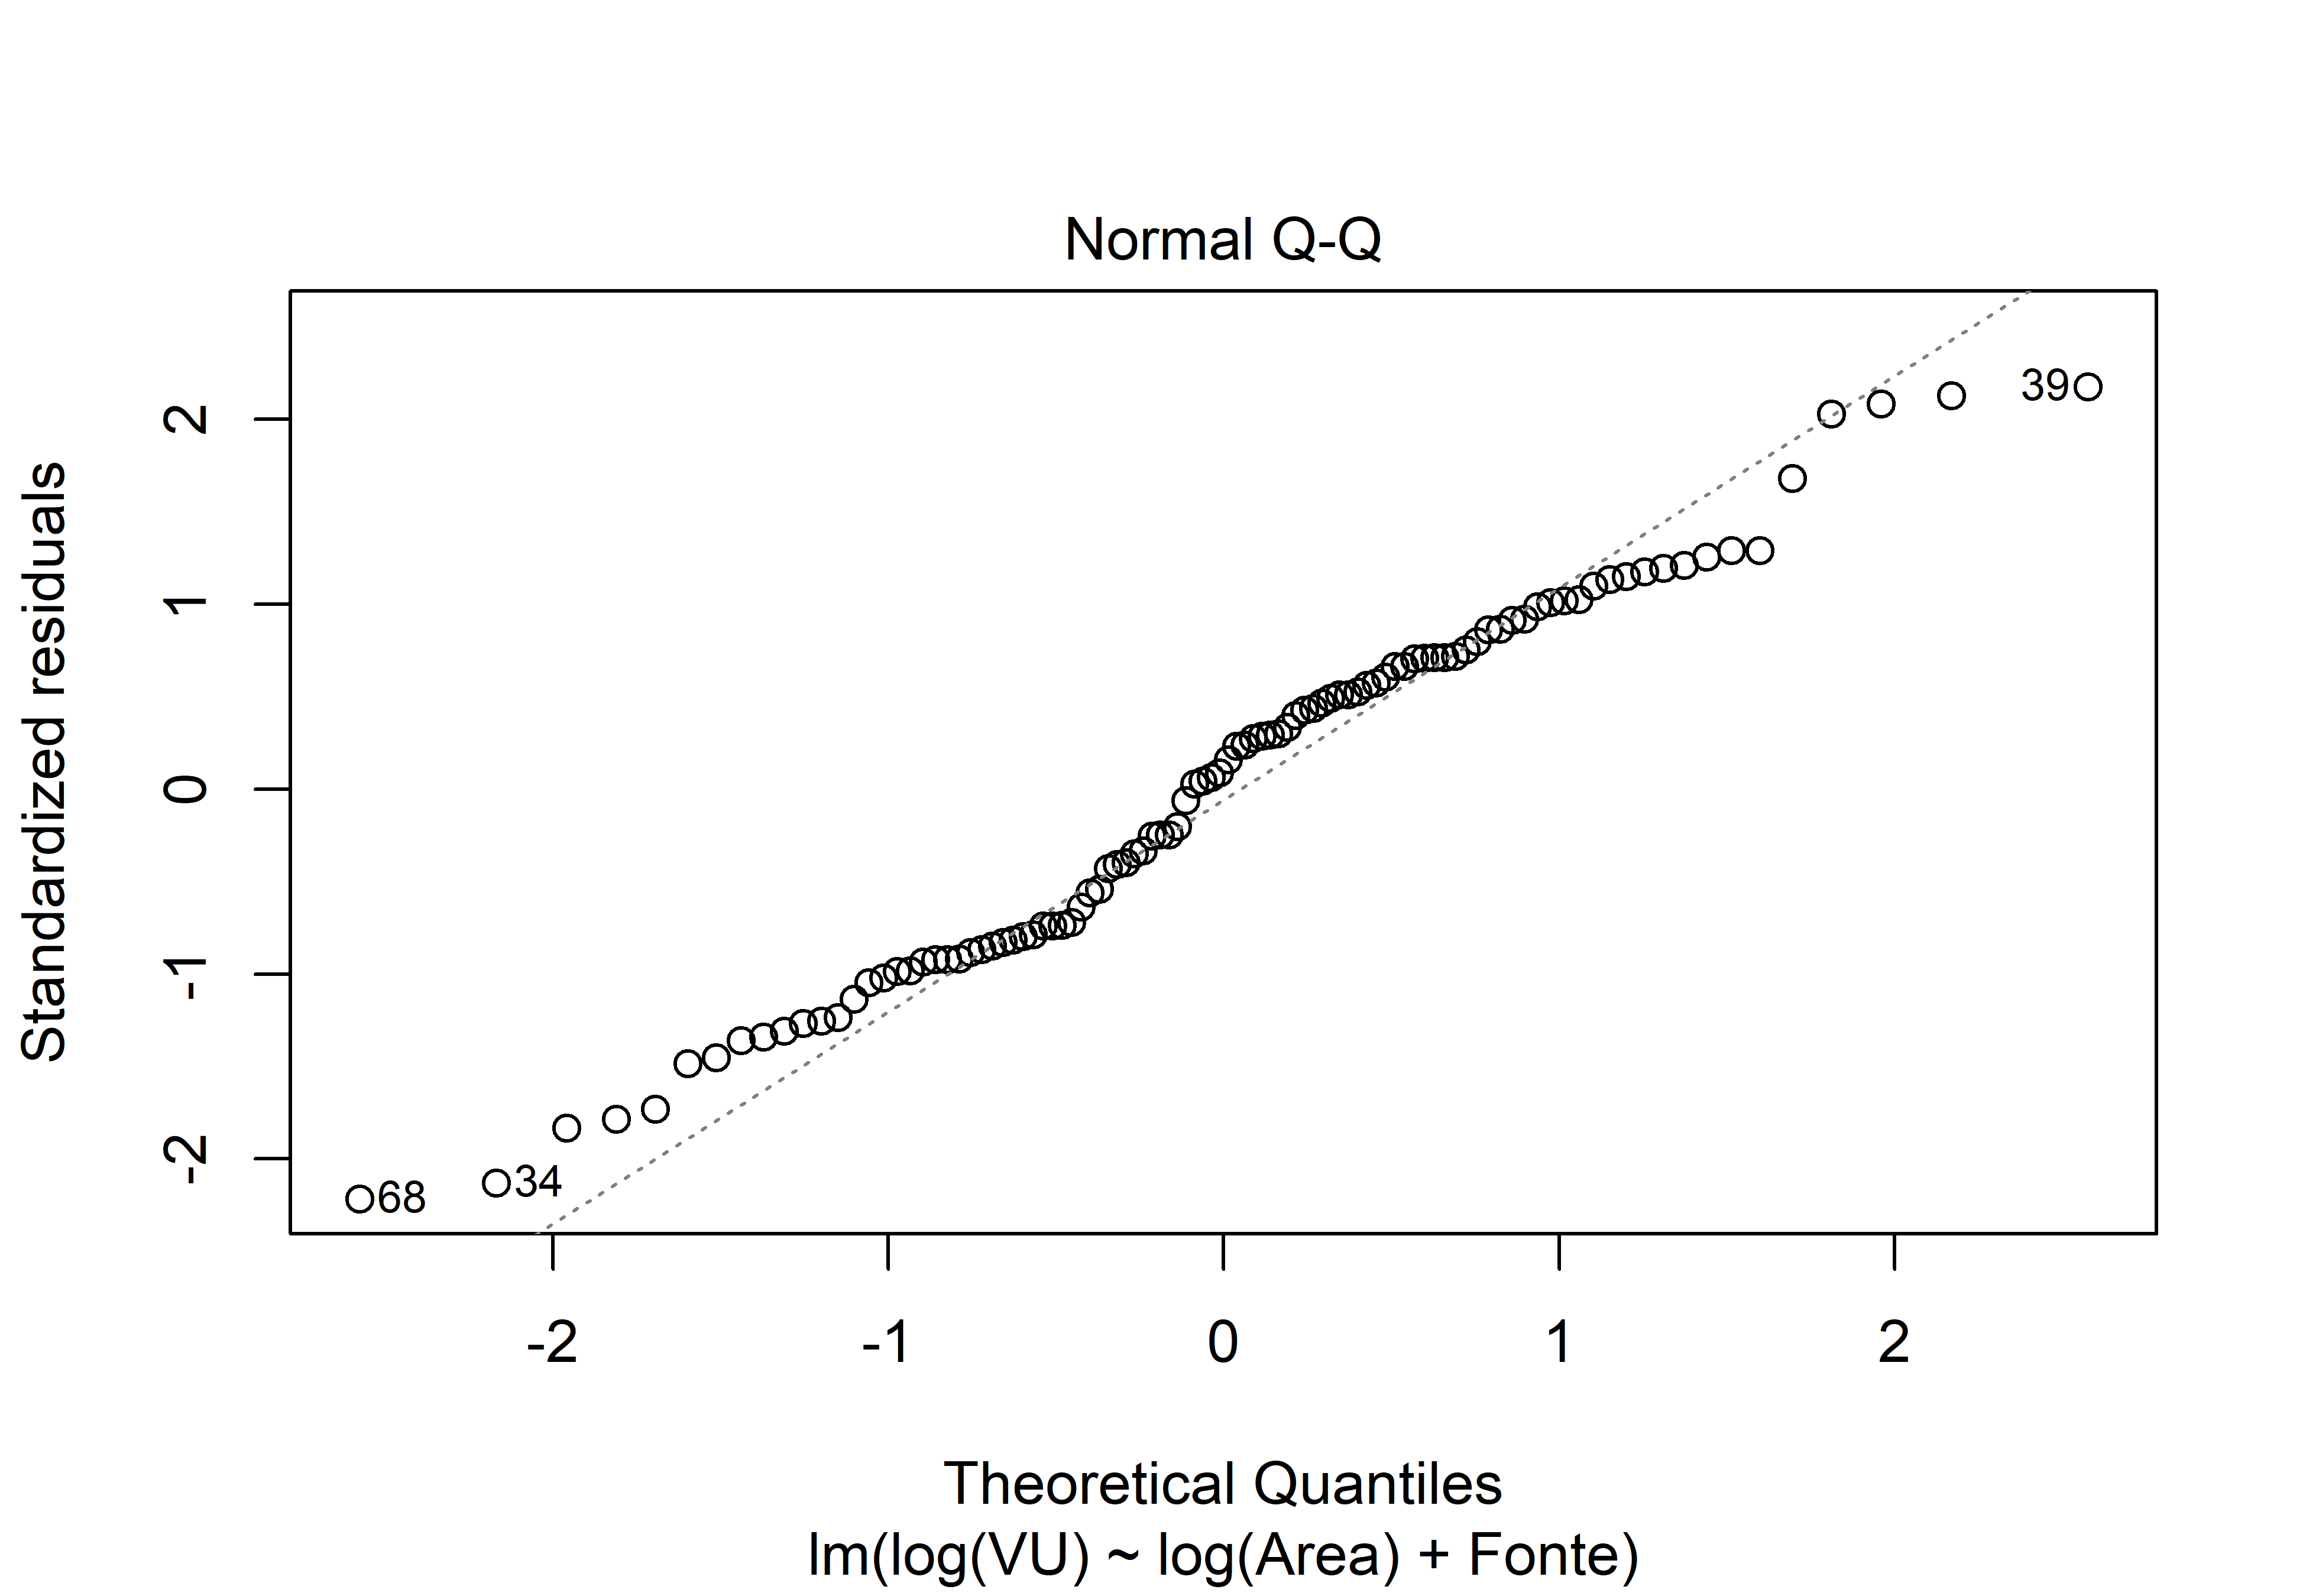
\includegraphics[width=0.5\linewidth]{./images/unnamed-chunk-28-2}
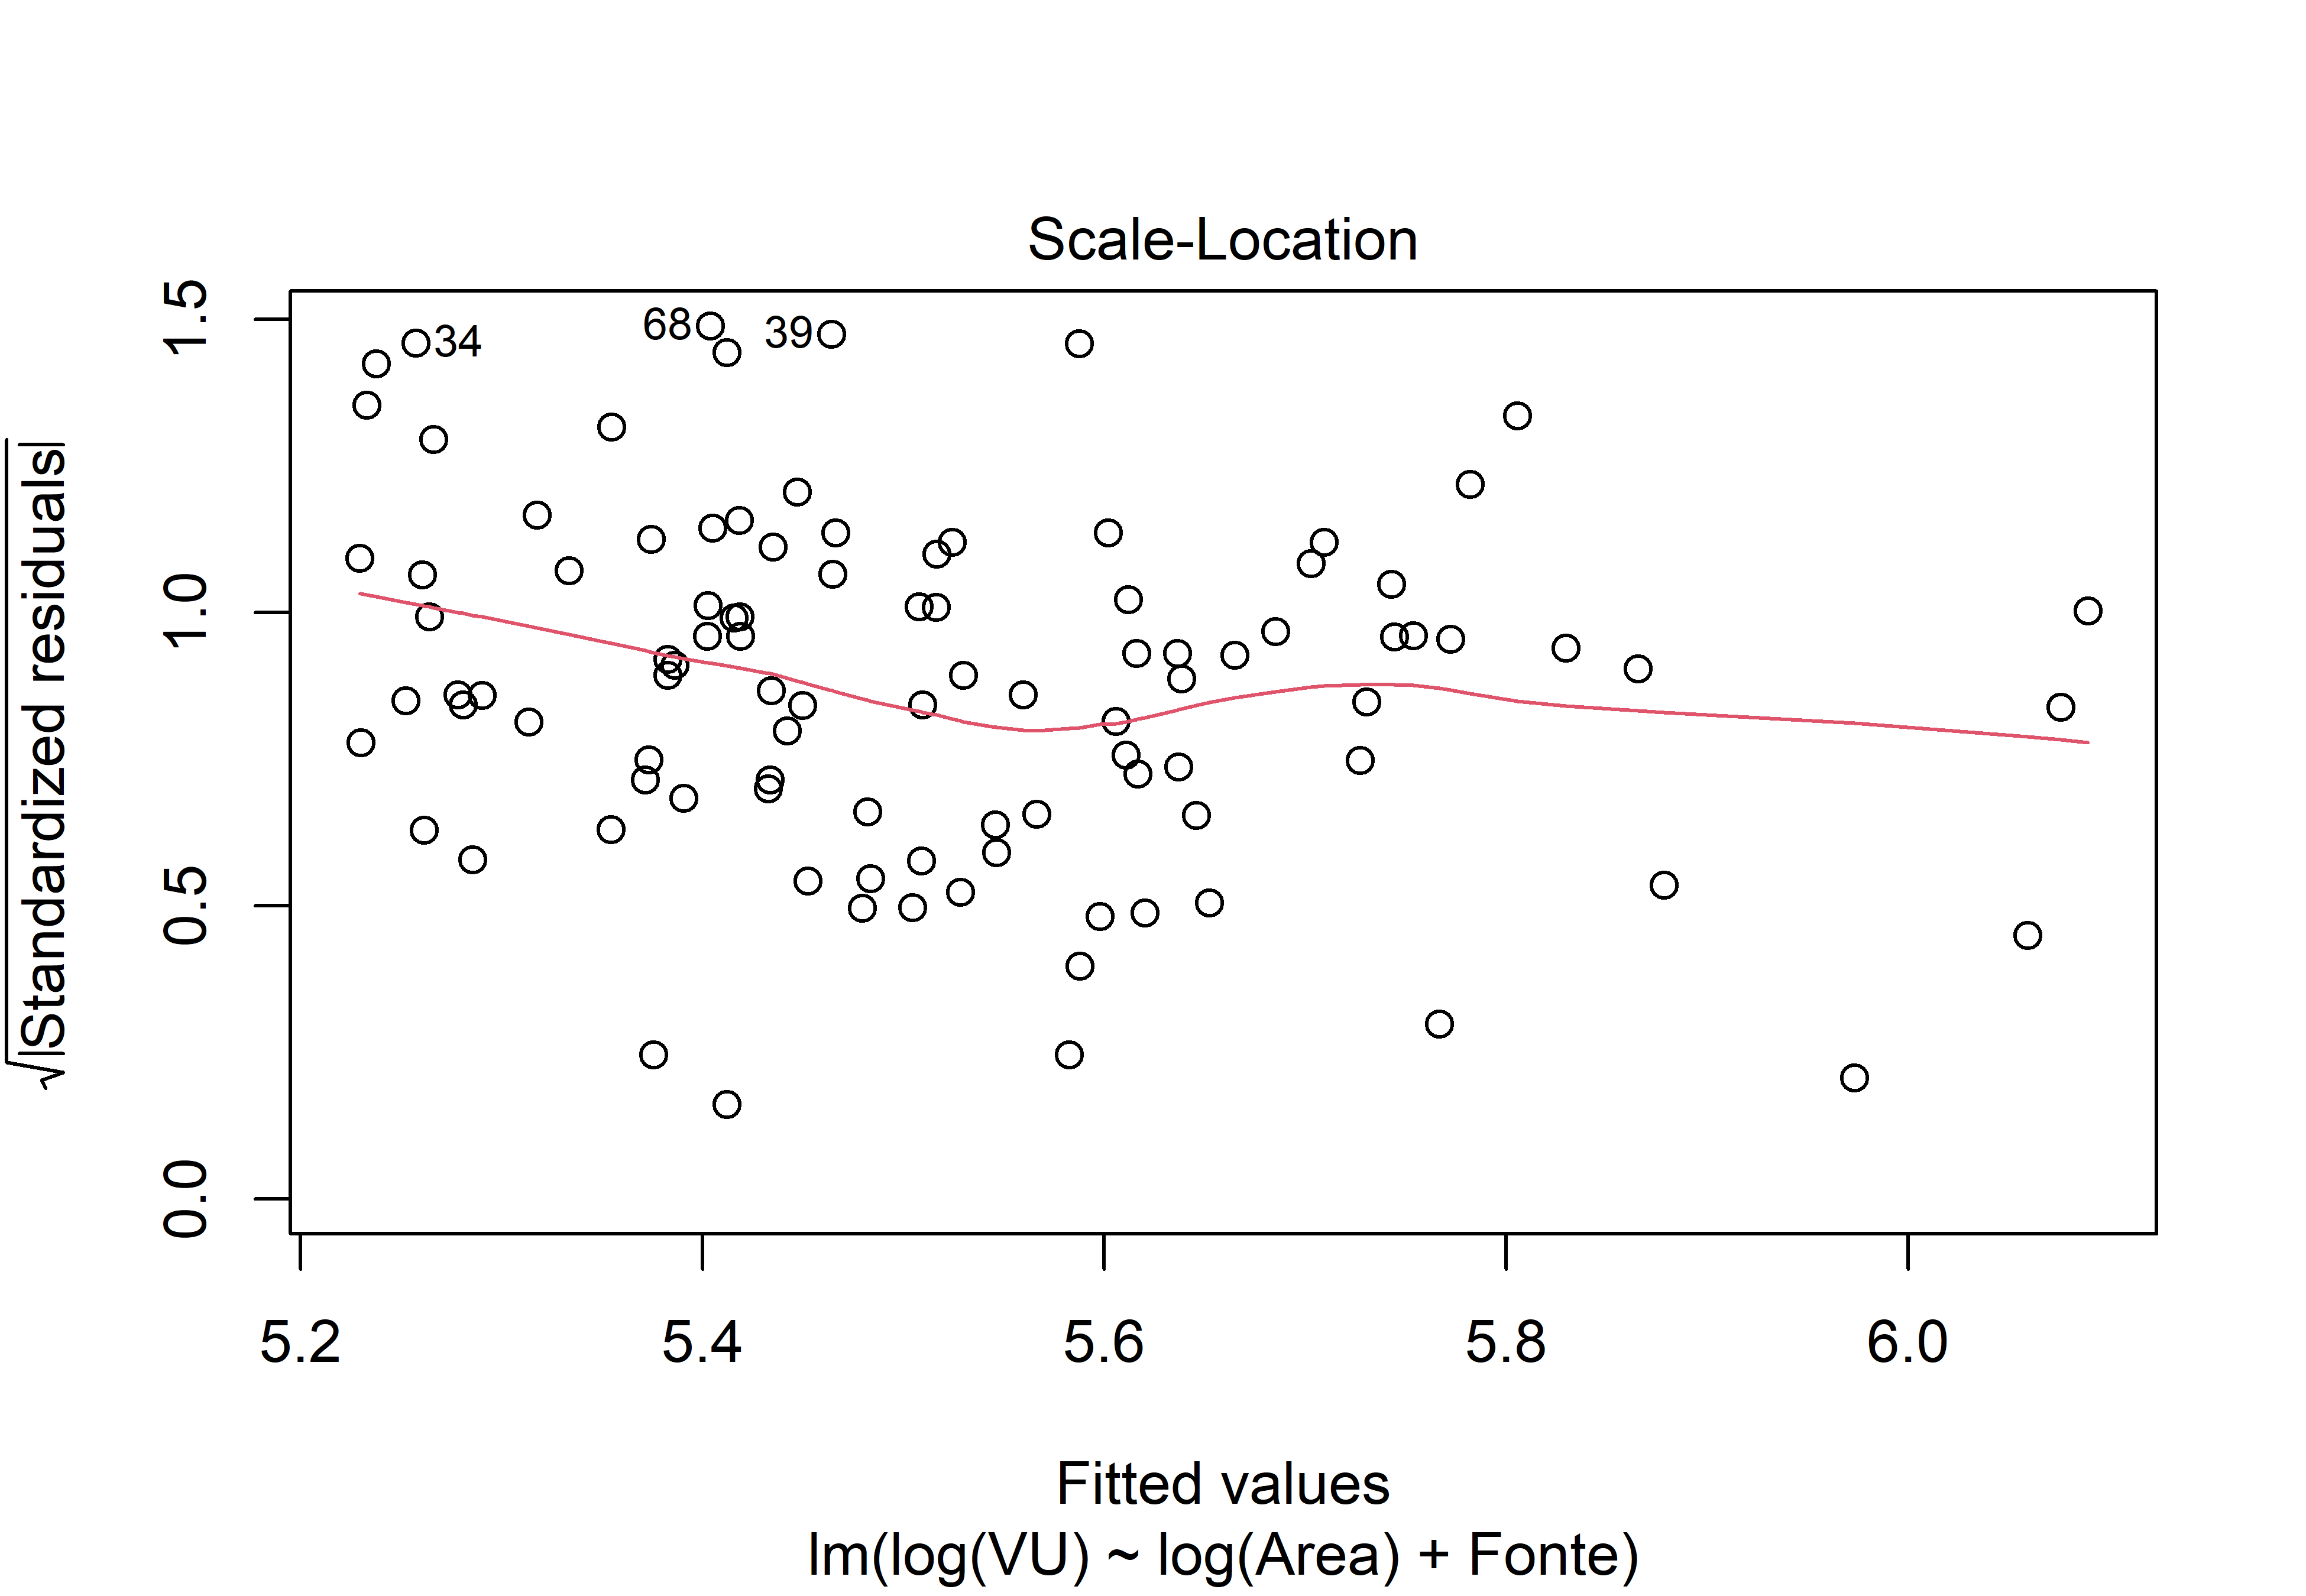
\includegraphics[width=0.5\linewidth]{./images/unnamed-chunk-28-3}
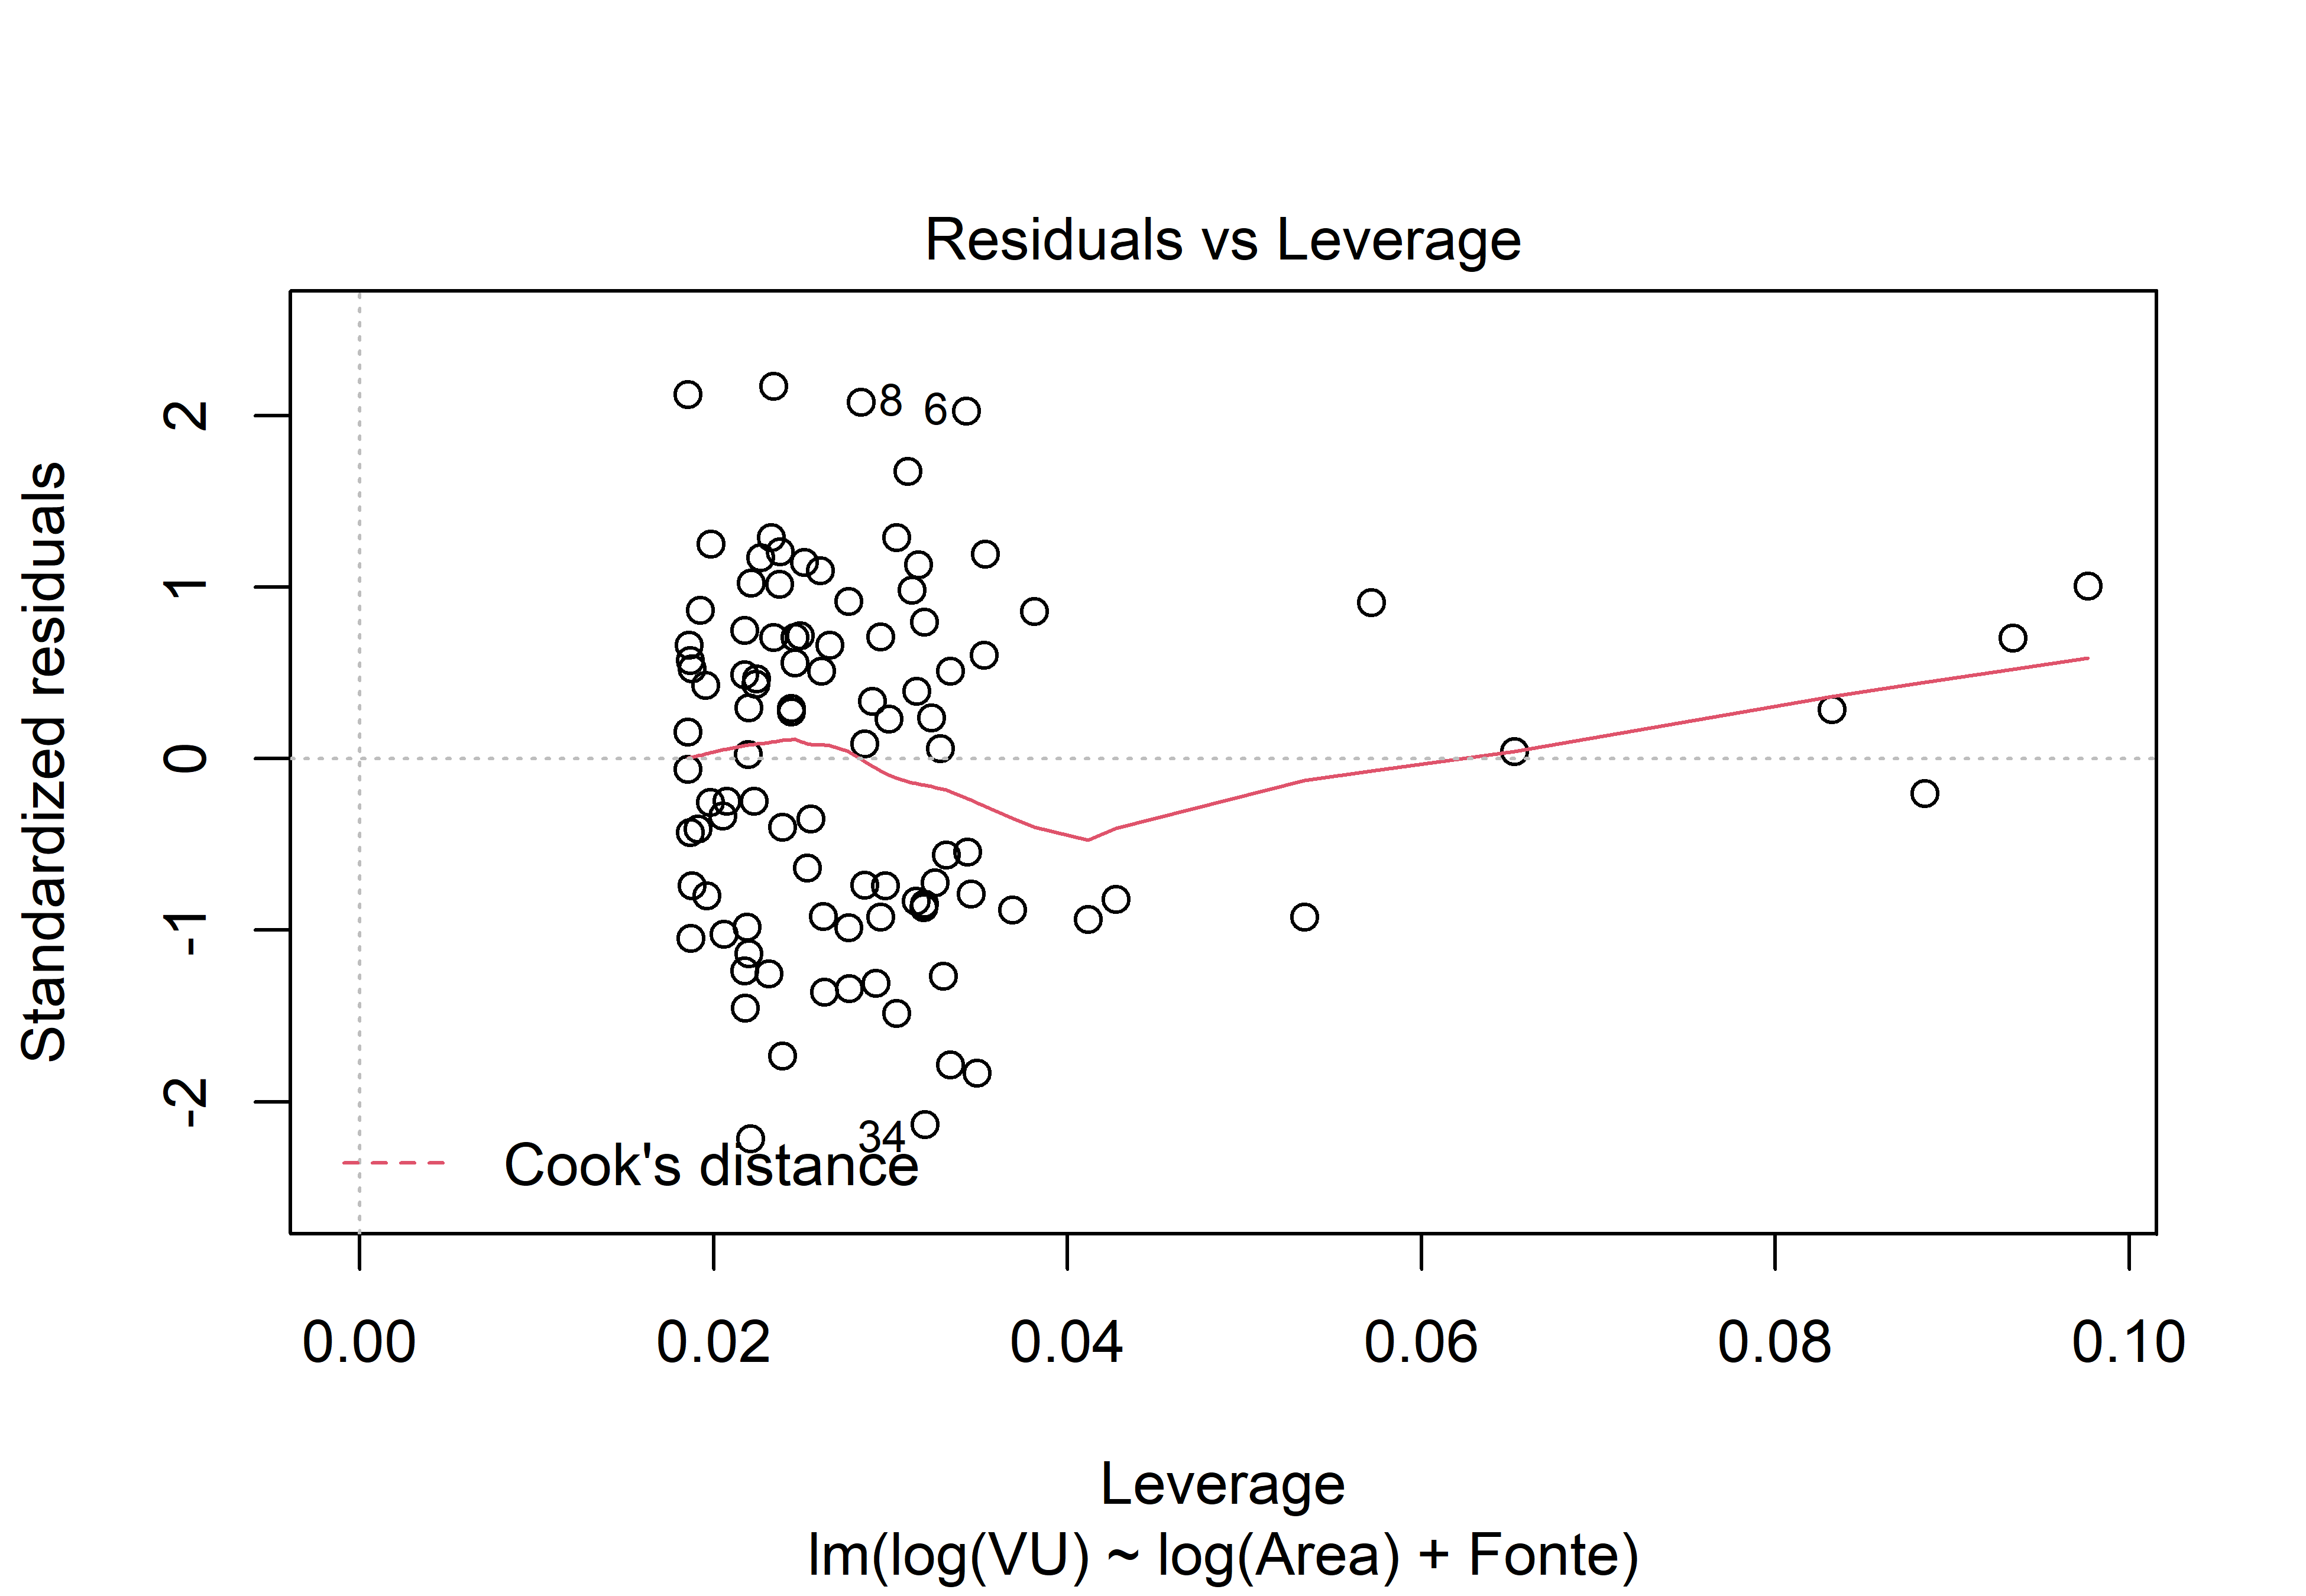
\includegraphics[width=0.5\linewidth]{./images/unnamed-chunk-28-4}

\begin{verbatim}
## 
##  studentized Breusch-Pagan test
## 
## data:  fit2
## BP = 4.4404, df = 2, p-value = 0.1086
\end{verbatim}

\begin{verbatim}
## `geom_smooth()` using method = 'loess' and formula 'y ~ x'
\end{verbatim}

\begin{verbatim}
## `geom_smooth()` using formula 'y ~ x'
\end{verbatim}

\begin{verbatim}
## `geom_smooth()` using method = 'loess' and formula 'y ~ x'
\end{verbatim}

\begin{figure}
\centering
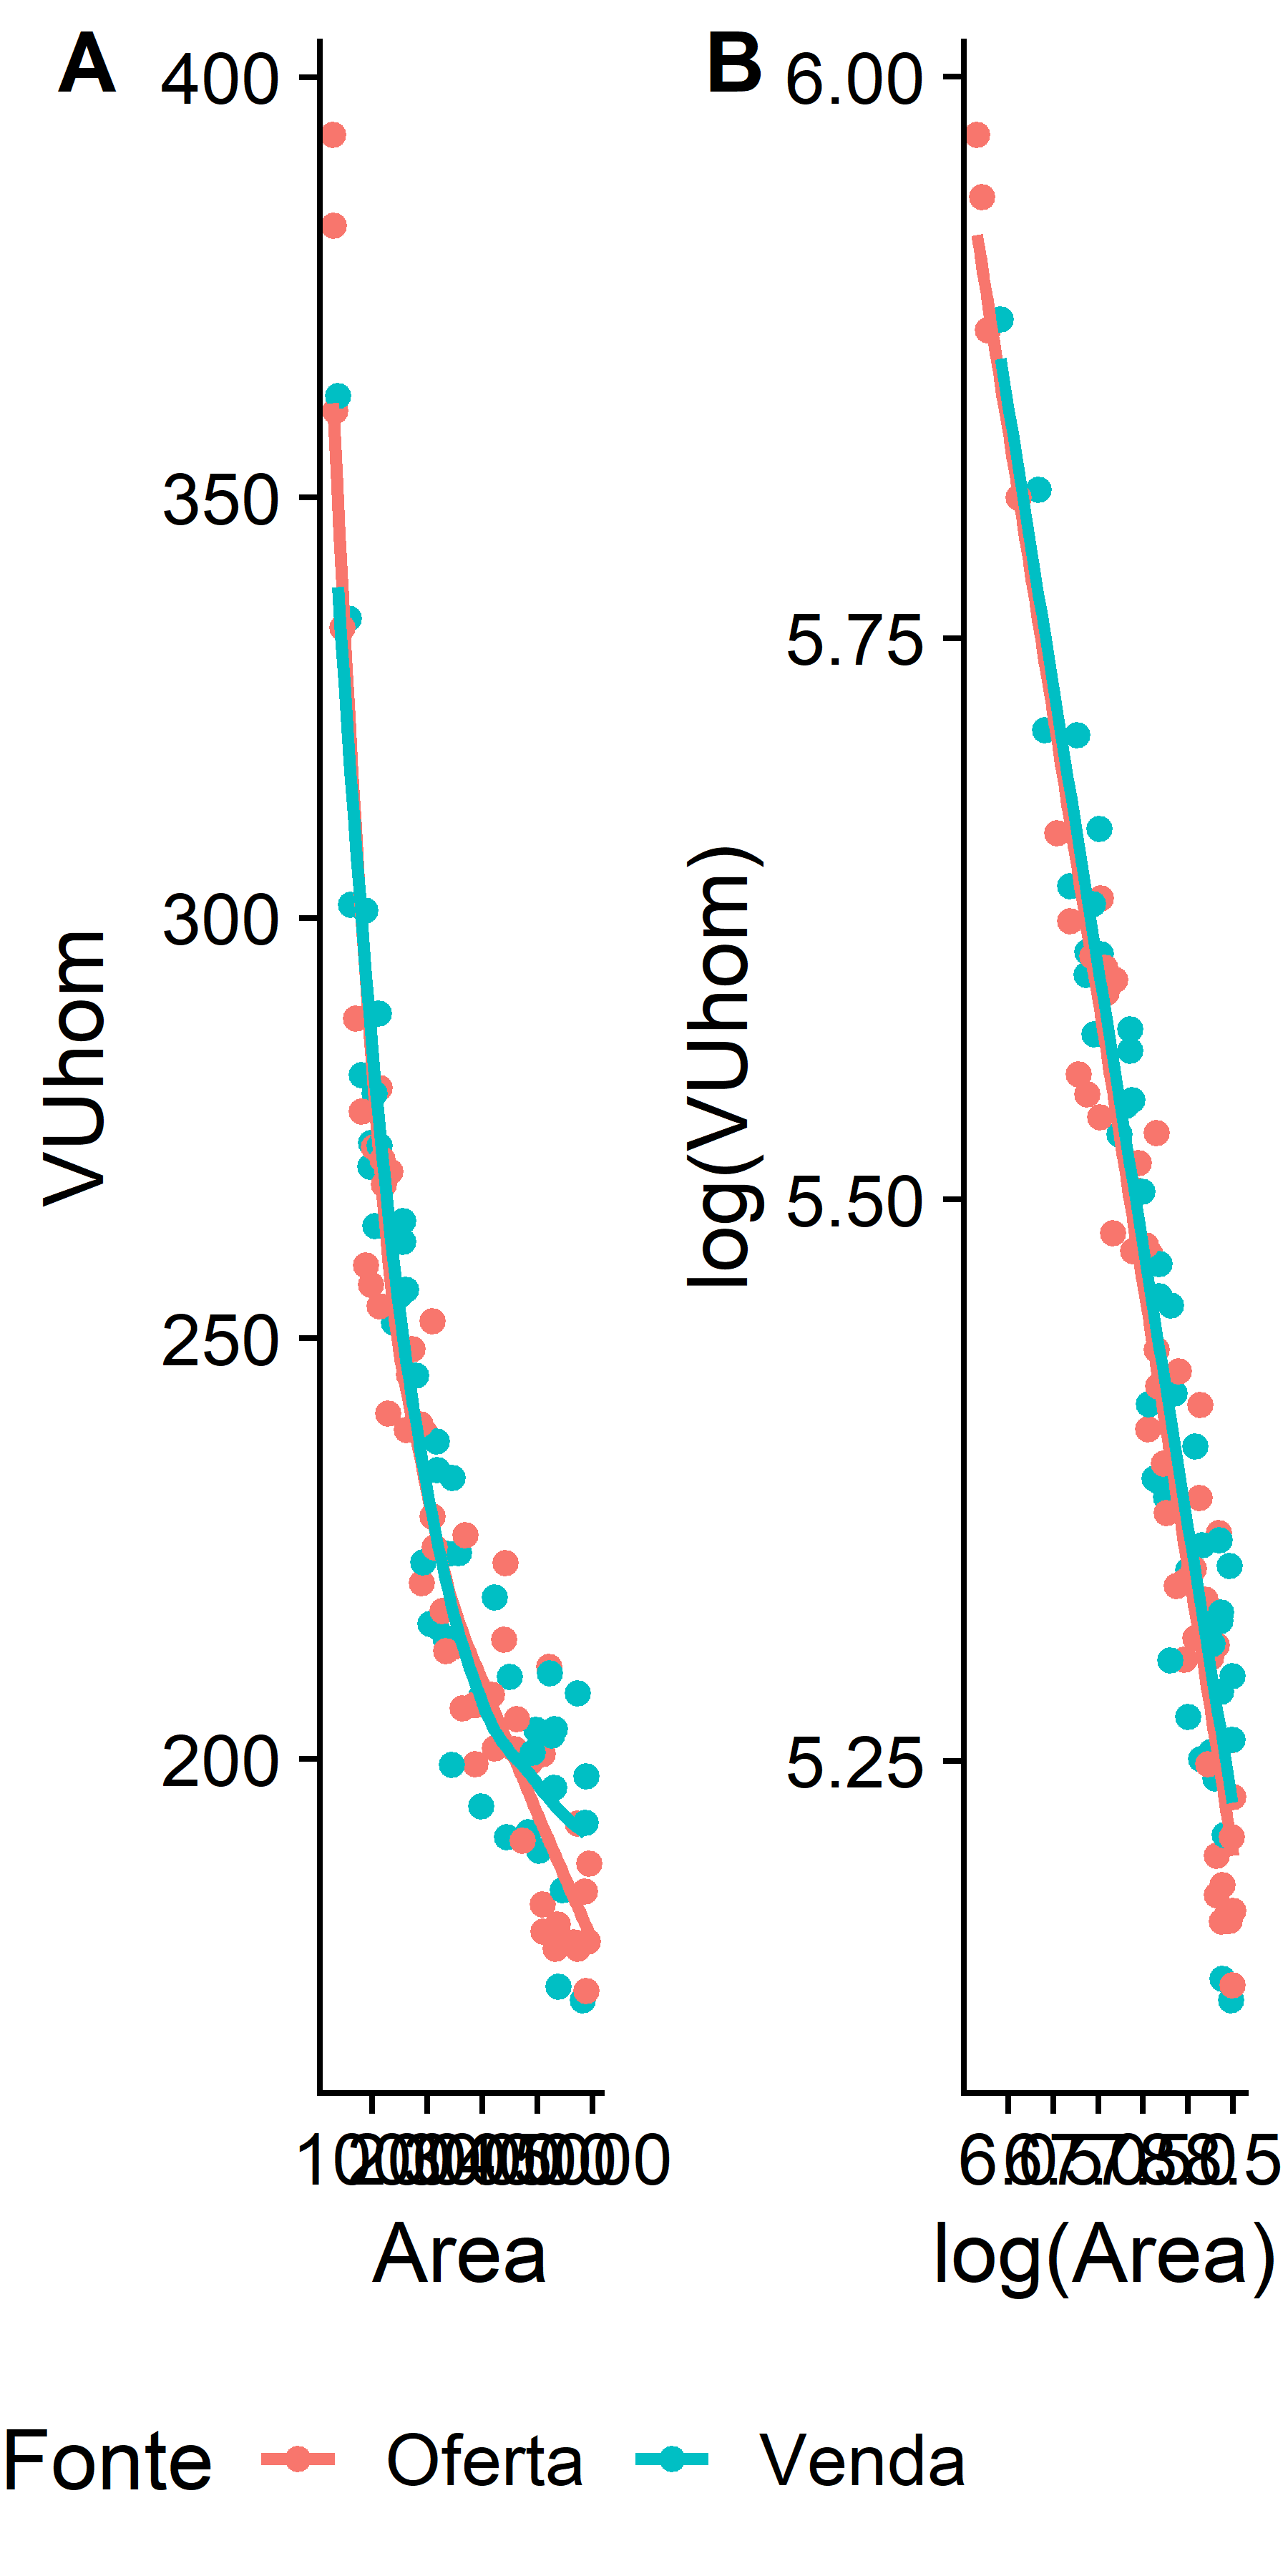
\includegraphics{./images/dadosHomogeneizados2-1.png}
\caption{Dados homogeneizados.}
\end{figure}

\begin{table}[H] \centering 
  \caption{Comparação dos modelos} 
  \label{} 
\begin{tabular}{@{\extracolsep{5pt}}lcc} 
\\[-1.8ex]\hline 
\hline \\[-1.8ex] 
 & \multicolumn{2}{c}{\textit{Dependent variable:}} \\ 
\cline{2-3} 
\\[-1.8ex] & log(VU) & log(VUhom) \\ 
\\[-1.8ex] & (1) & (2)\\ 
\hline \\[-1.8ex] 
 Constant & 7,51 (7,44, 7,58) & 7,35 (7,28, 7,42) \\ 
  & t = 138,99$^{***}$ & t = 134,98$^{***}$ \\ 
  log(Area) & $-$0,25 ($-$0,26, $-$0,24) & $-$0,25 ($-$0,26, $-$0,24) \\ 
  & t = $-$35,80$^{***}$ & t = $-$35,40$^{***}$ \\ 
  FonteVenda & $-$0,15 ($-$0,16, $-$0,13) &  \\ 
  & t = $-$14,54$^{***}$ &  \\ 
 \hline \\[-1.8ex] 
Observations & 100 & 100 \\ 
R$^{2}$ & 0,94 & 0,93 \\ 
Adjusted R$^{2}$ & 0,94 & 0,93 \\ 
Residual Std. Error & 0,05 (df = 97) & 0,05 (df = 98) \\ 
F Statistic & 756,28$^{***}$ (df = 2; 97) & 1.253,45$^{***}$ (df = 1; 98) \\ 
\hline 
\hline \\[-1.8ex] 
Notas: & \multicolumn{2}{r}{$^{*}$p$<$0,3; $^{**}$p$<$0,2; $^{***}$p$<$0,1} \\ 
\end{tabular} 
\end{table}

\begin{center}\rule{0.5\linewidth}{0.5pt}\end{center}

\begin{verbatim}
## `geom_smooth()` using method = 'loess' and formula 'y ~ x'
## `geom_smooth()` using method = 'loess' and formula 'y ~ x'
## `geom_smooth()` using method = 'loess' and formula 'y ~ x'
\end{verbatim}

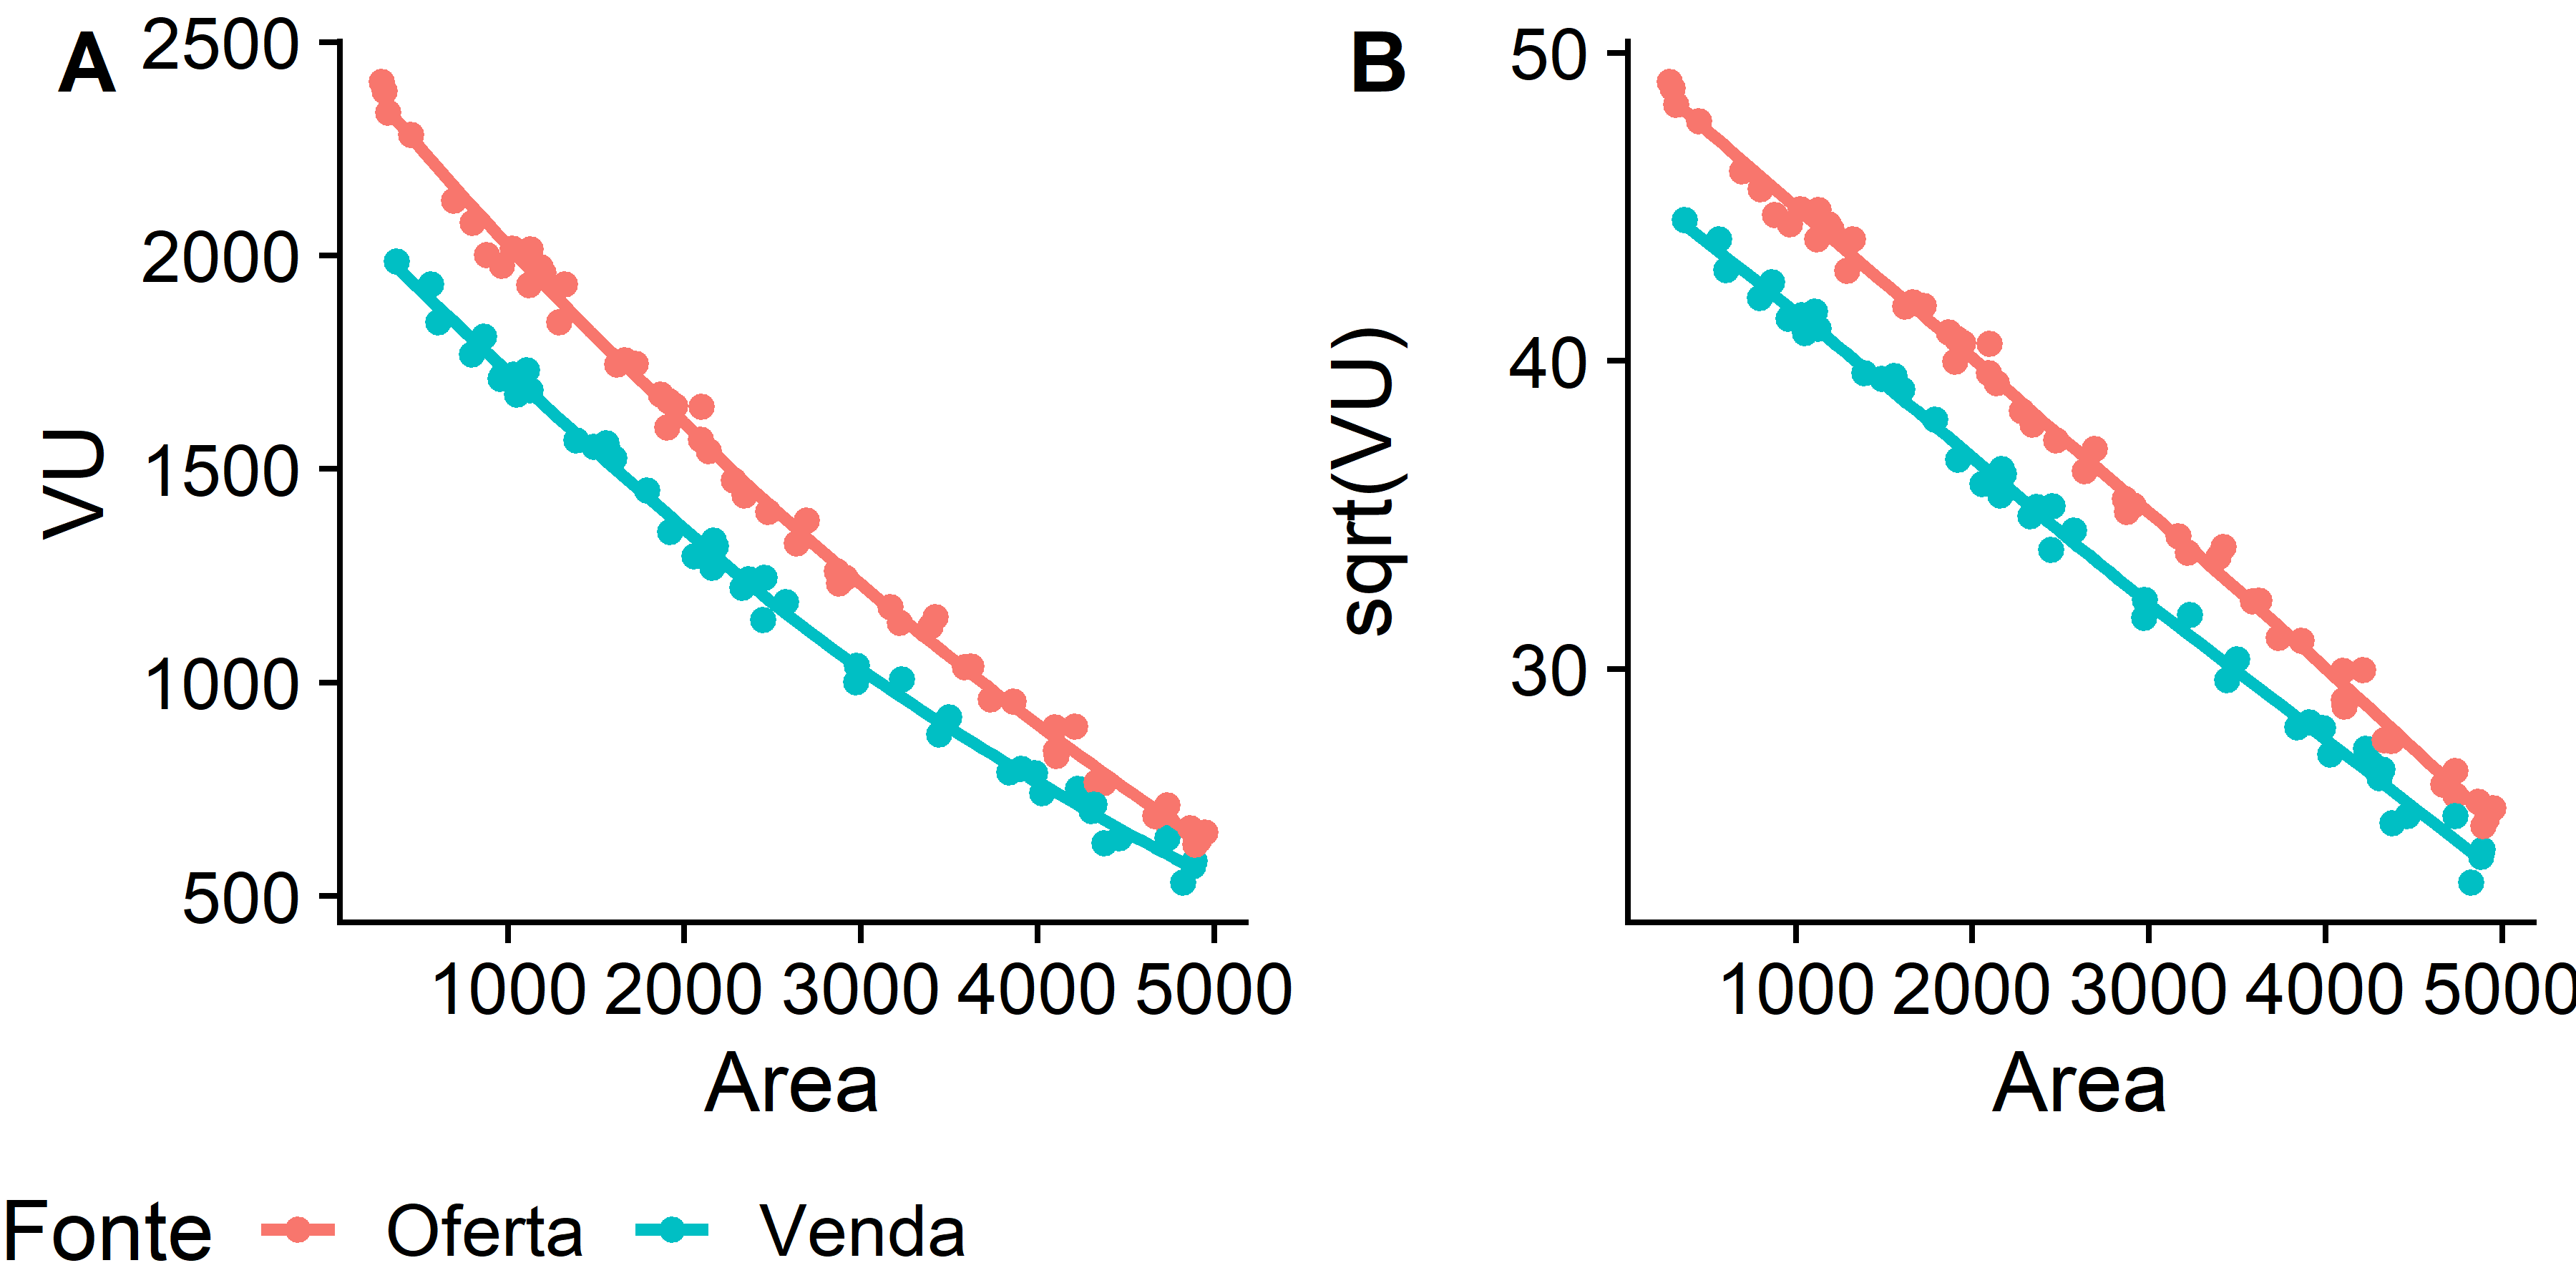
\includegraphics{./images/unnamed-chunk-32-1.png}

\begin{verbatim}
## 
## Call:
## lm(formula = sqrt(VU) ~ Area + Fonte, data = dados)
## 
## Residuals:
##      Min       1Q   Median       3Q      Max 
## -1.03545 -0.41809 -0.02231  0.41313  1.37505 
## 
## Coefficients:
##               Estimate Std. Error t value Pr(>|t|)    
## (Intercept)  4.955e+01  1.292e-01  383.47   <2e-16 ***
## Area        -4.828e-03  4.006e-05 -120.51   <2e-16 ***
## FonteVenda  -2.848e+00  1.134e-01  -25.11   <2e-16 ***
## ---
## Signif. codes:  0 '***' 0.001 '**' 0.01 '*' 0.05 '.' 0.1 ' ' 1
## 
## Residual standard error: 0.5652 on 97 degrees of freedom
## Multiple R-squared:  0.9936, Adjusted R-squared:  0.9935 
## F-statistic:  7562 on 2 and 97 DF,  p-value: < 2.2e-16
\end{verbatim}

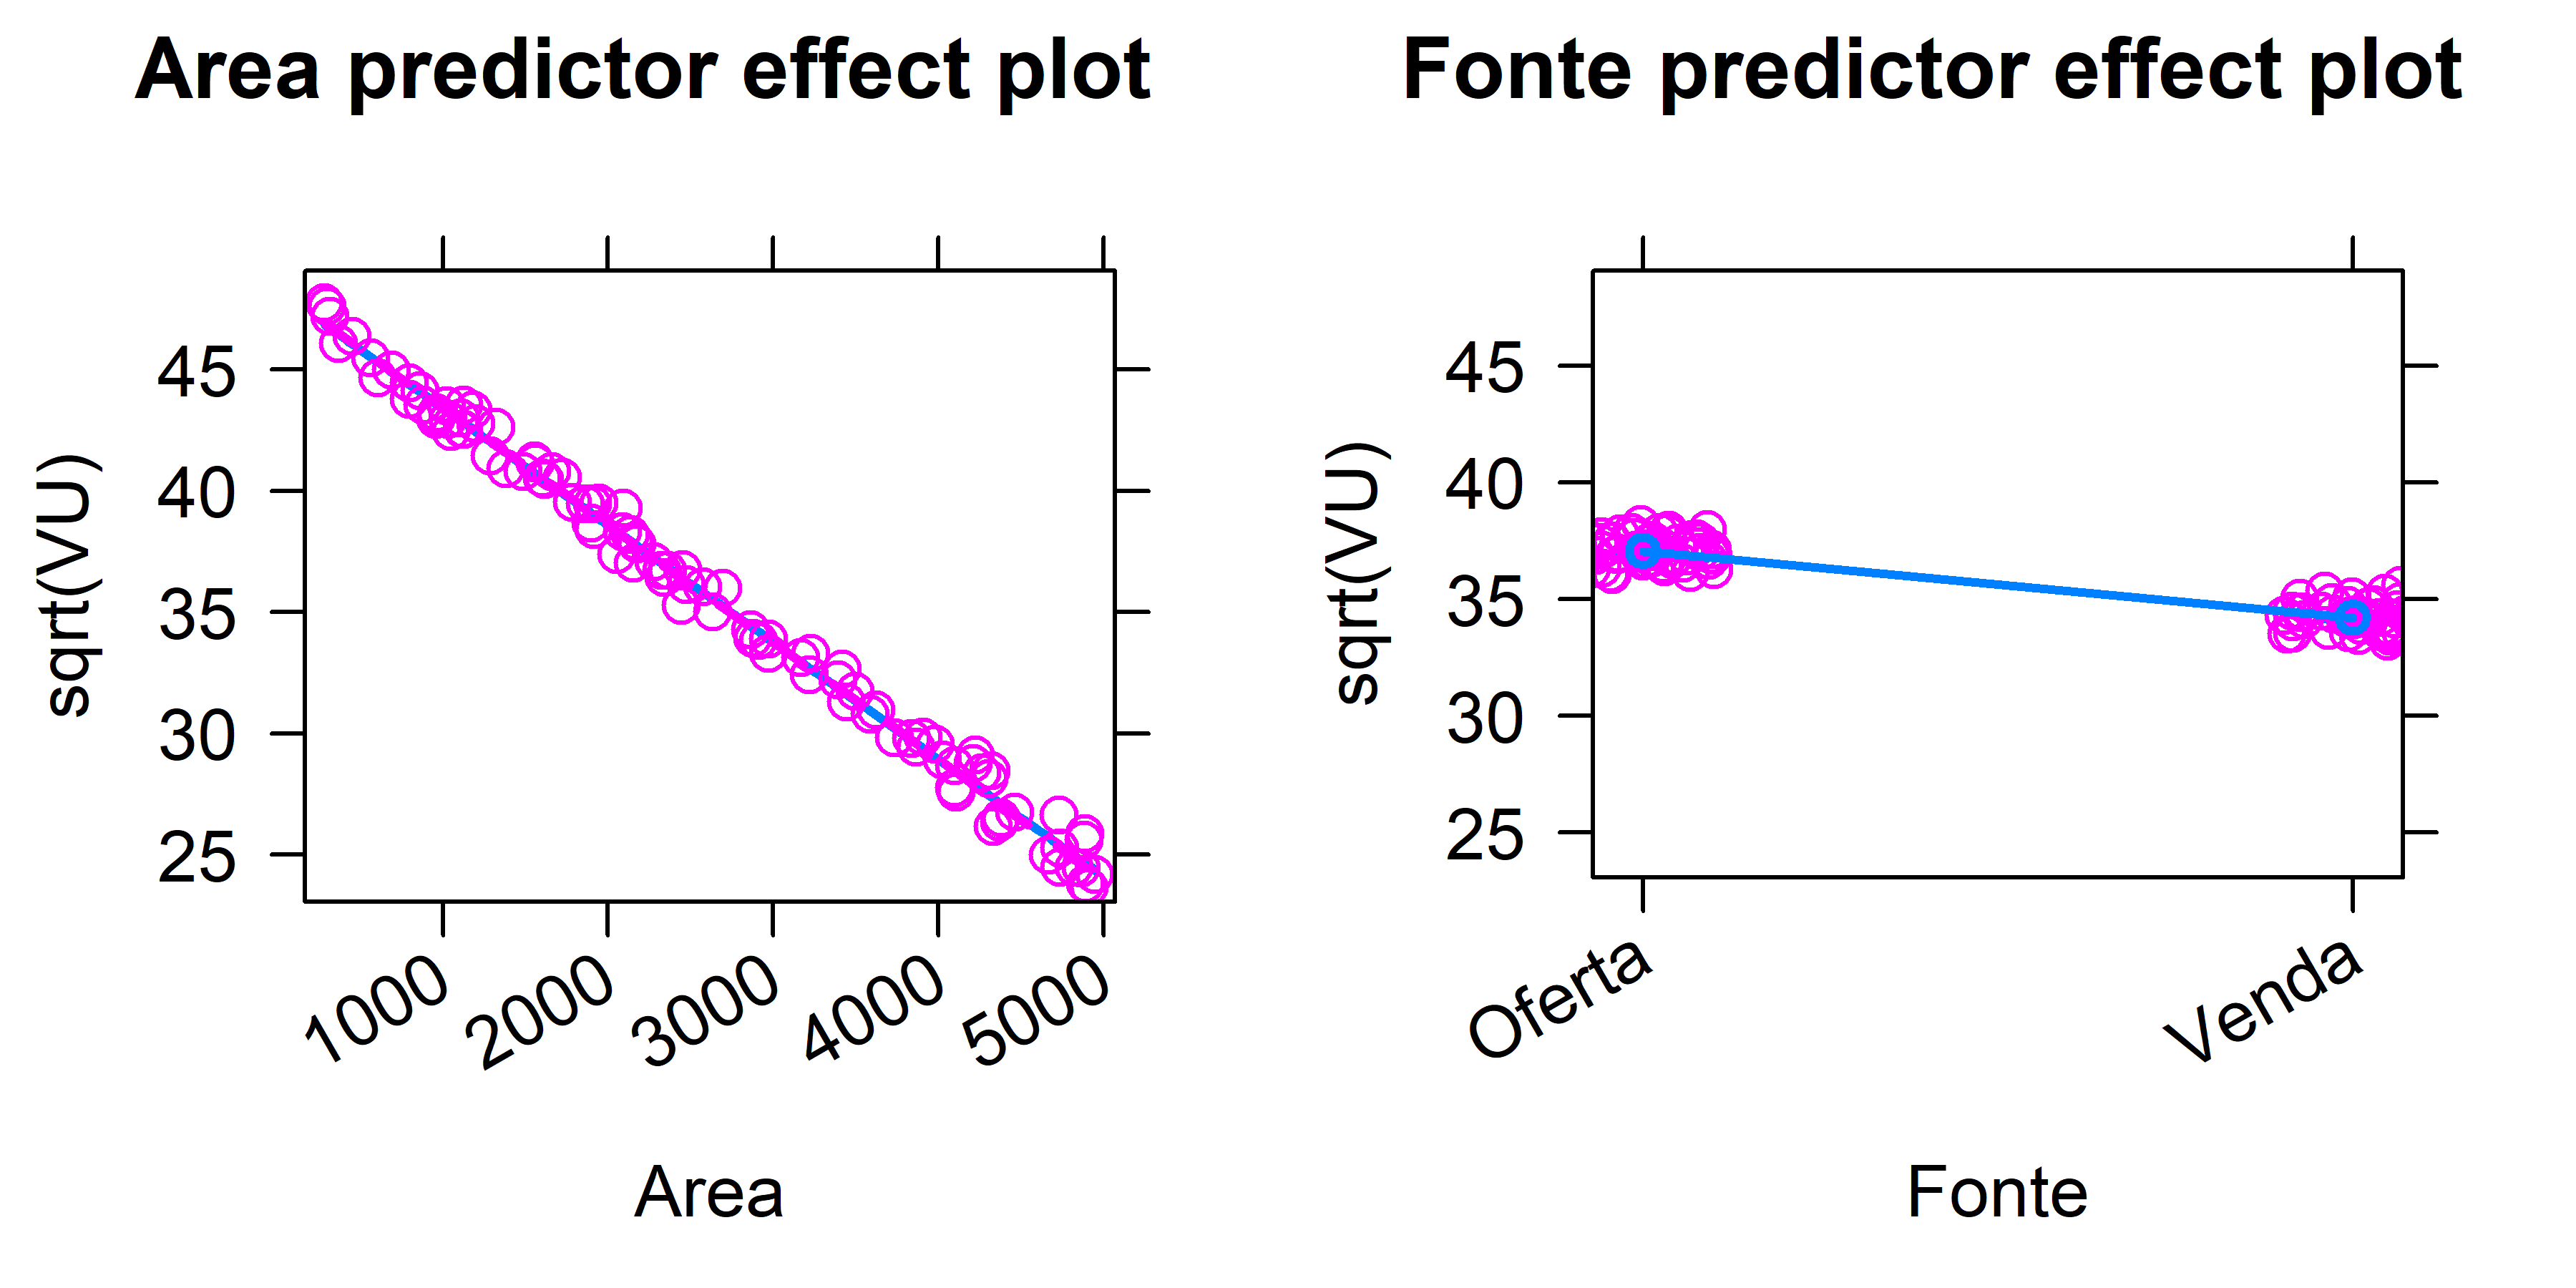
\includegraphics{./images/unnamed-chunk-34-1.png}

\begin{figure}[H]
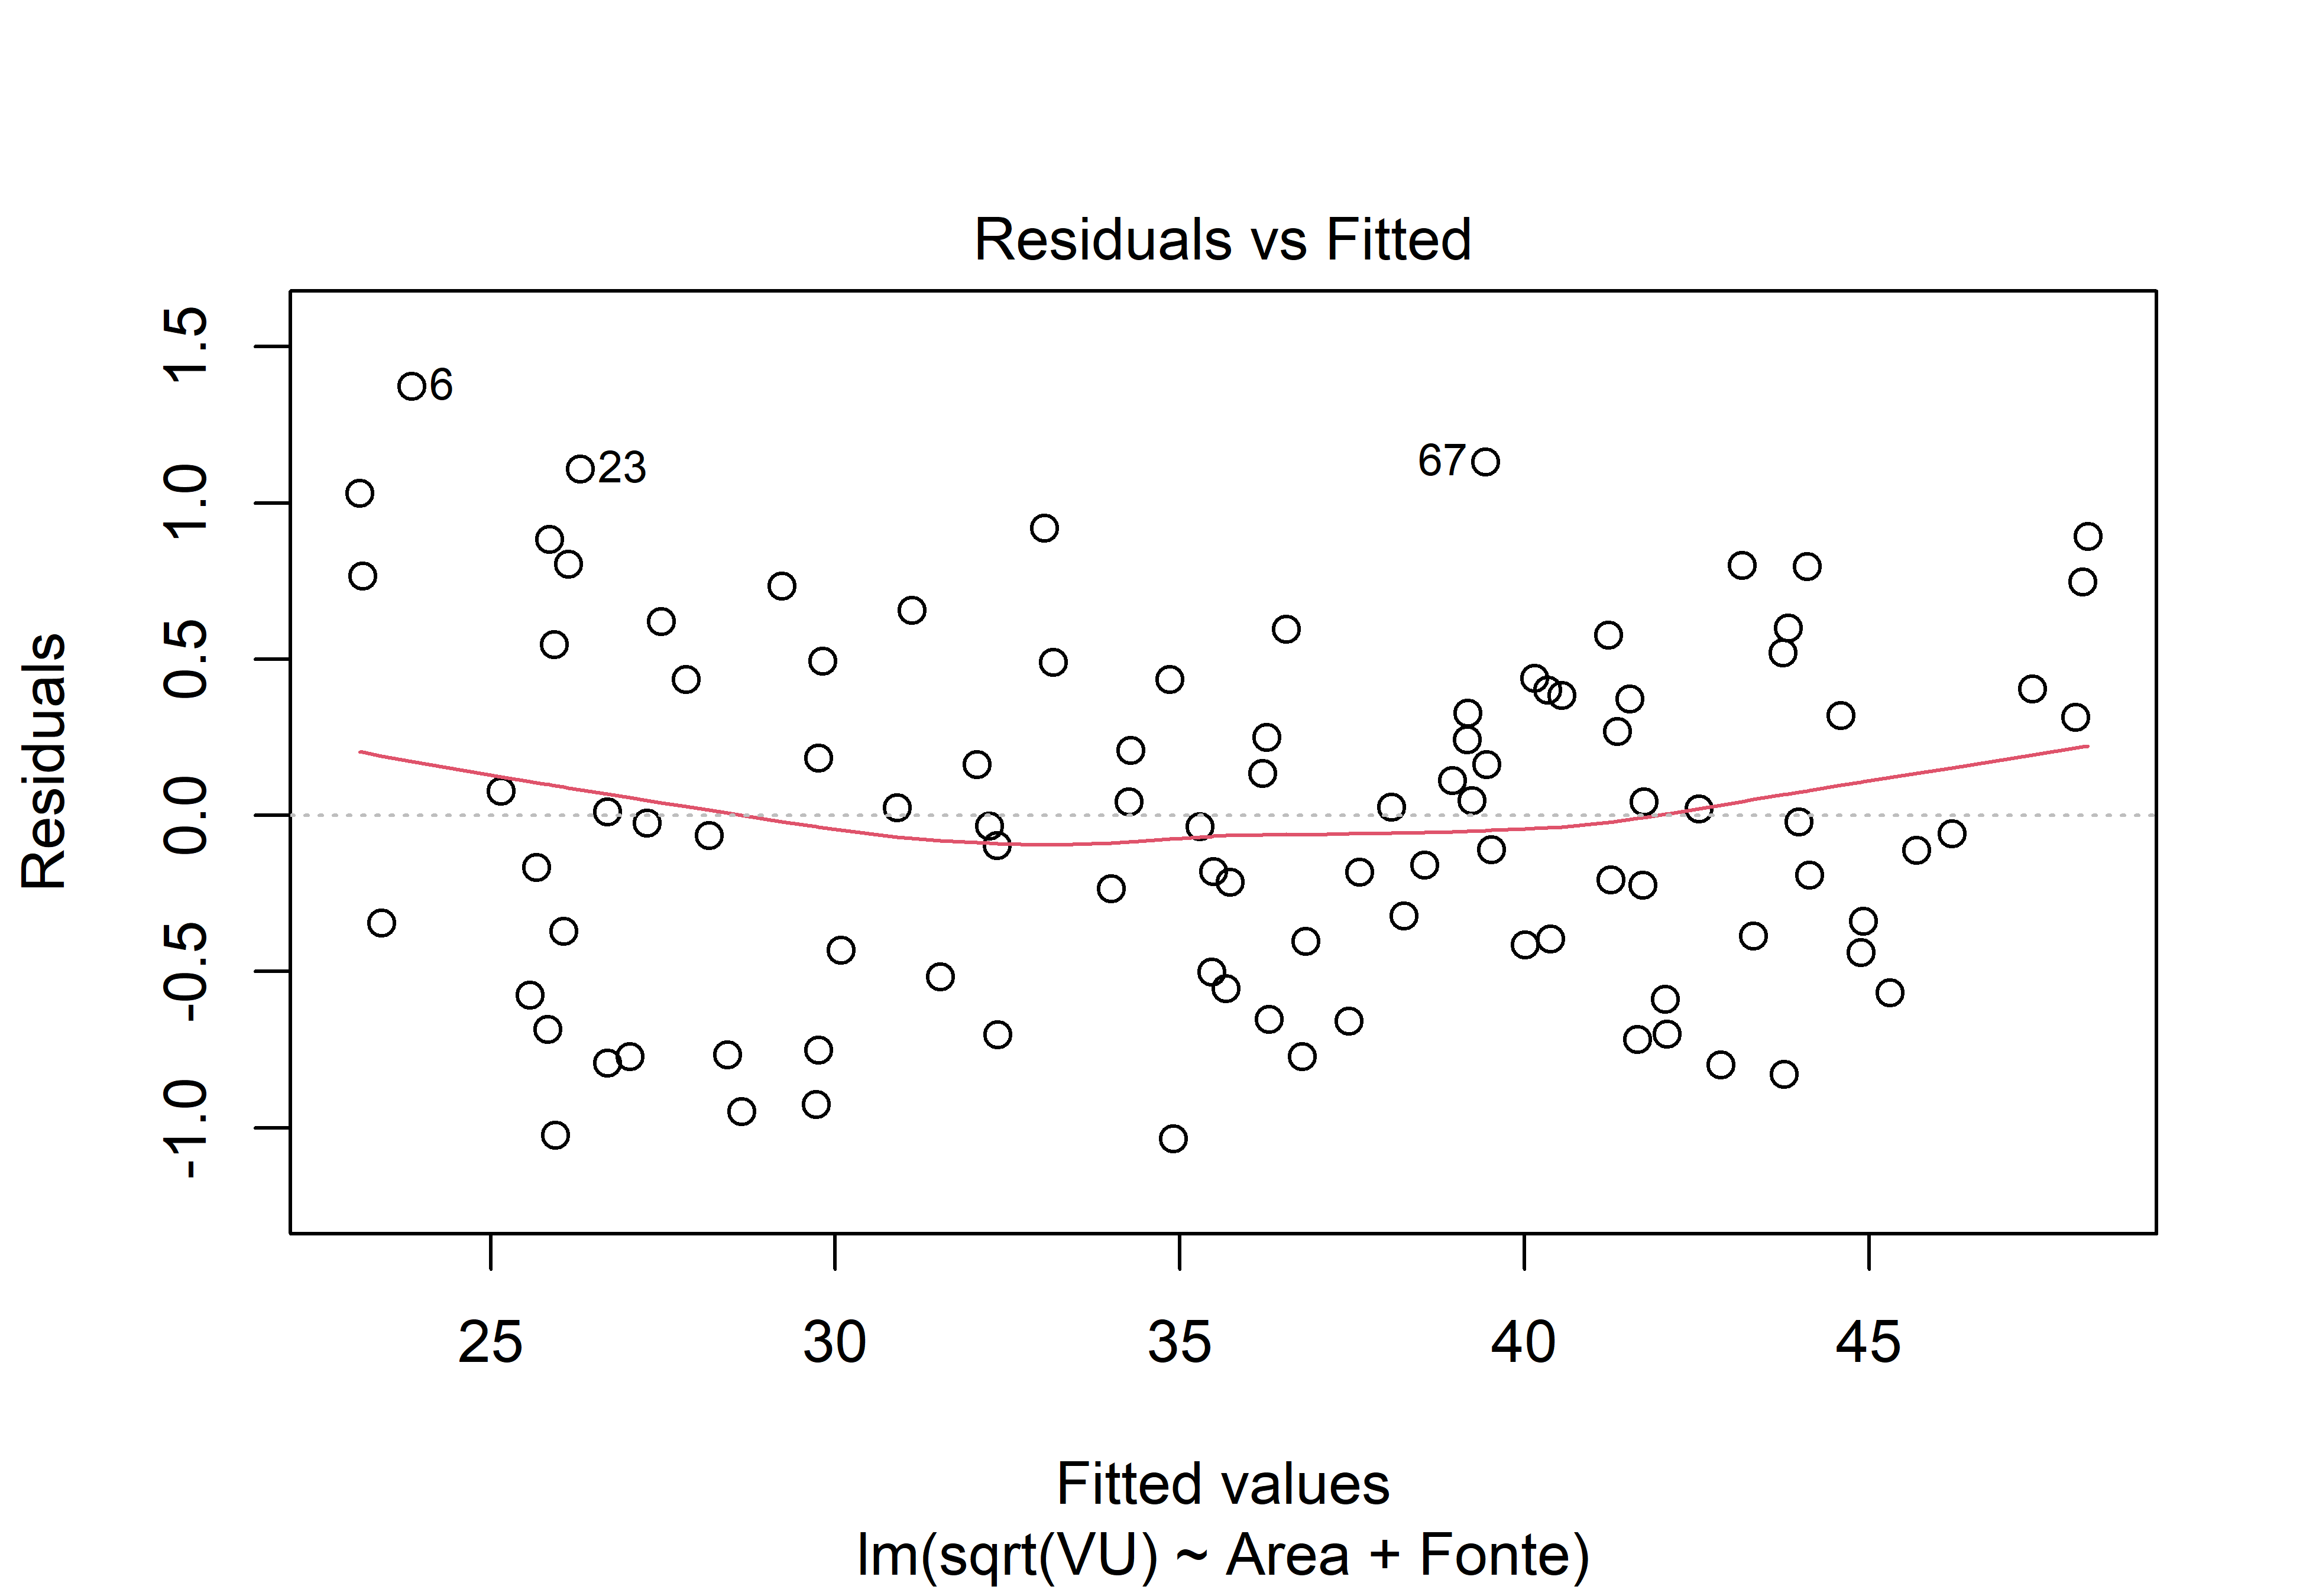
\includegraphics[width=0.5\linewidth]{./images/fit3Diagnostics-1} 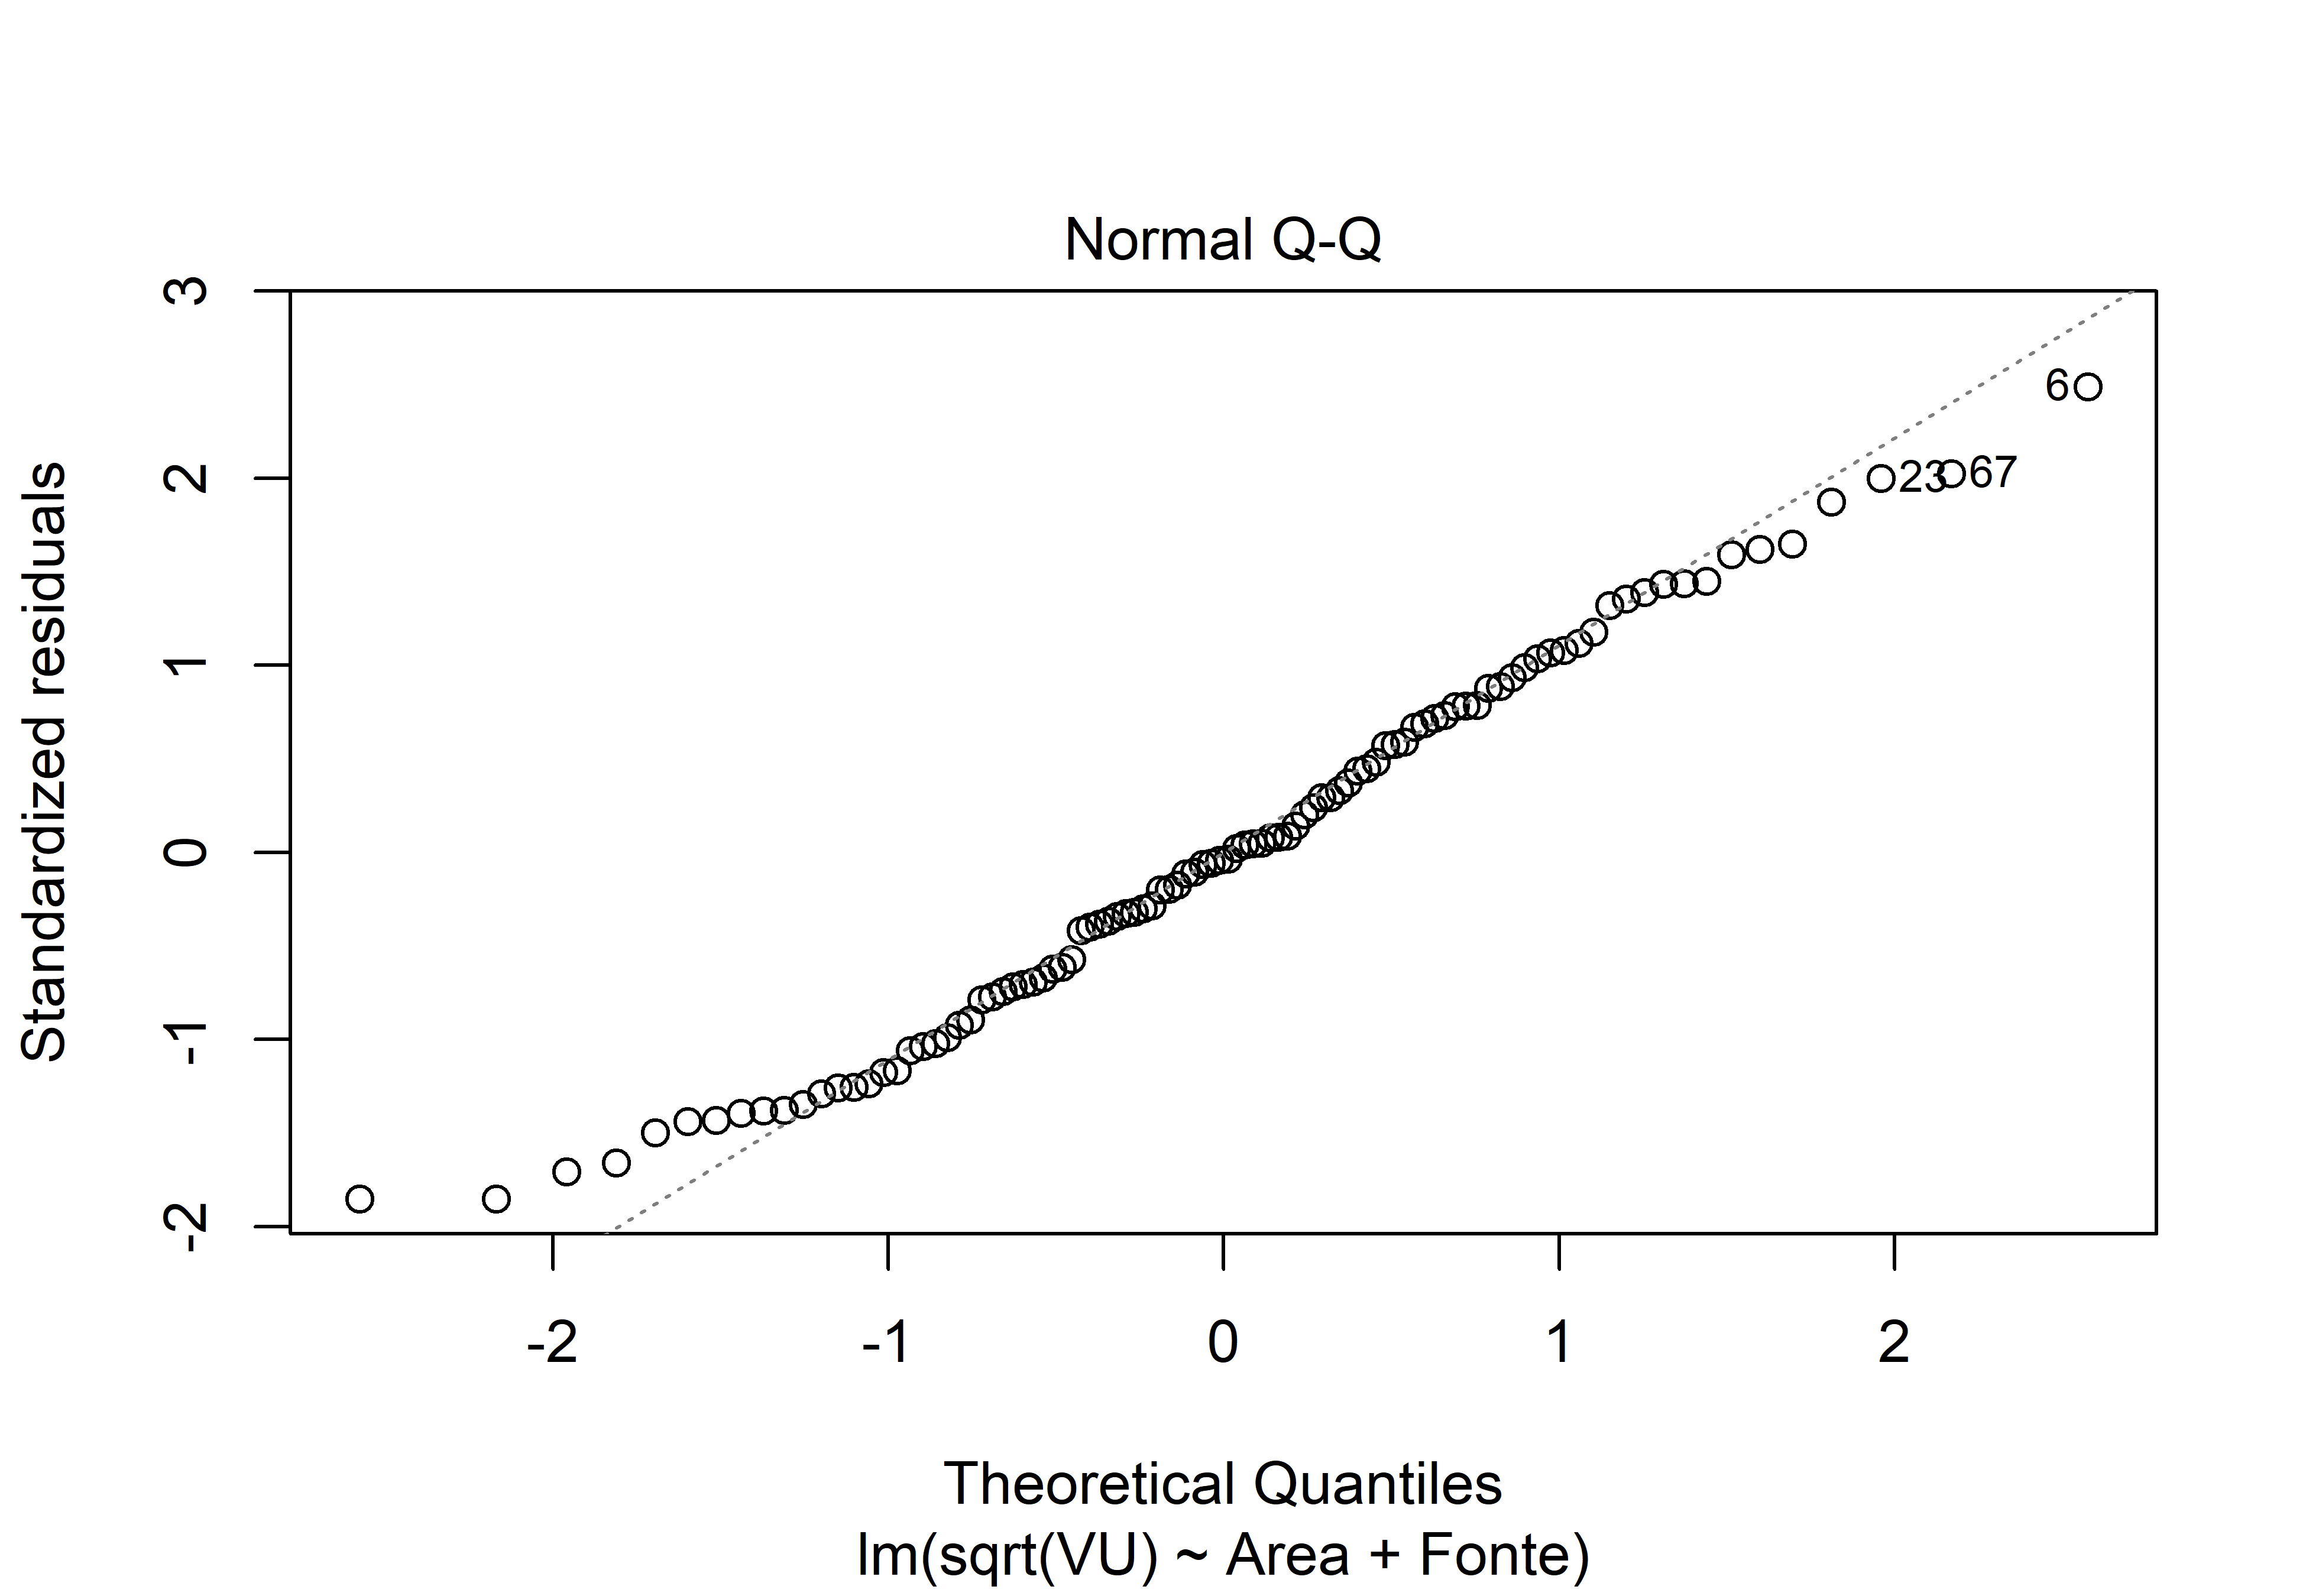
\includegraphics[width=0.5\linewidth]{./images/fit3Diagnostics-2} 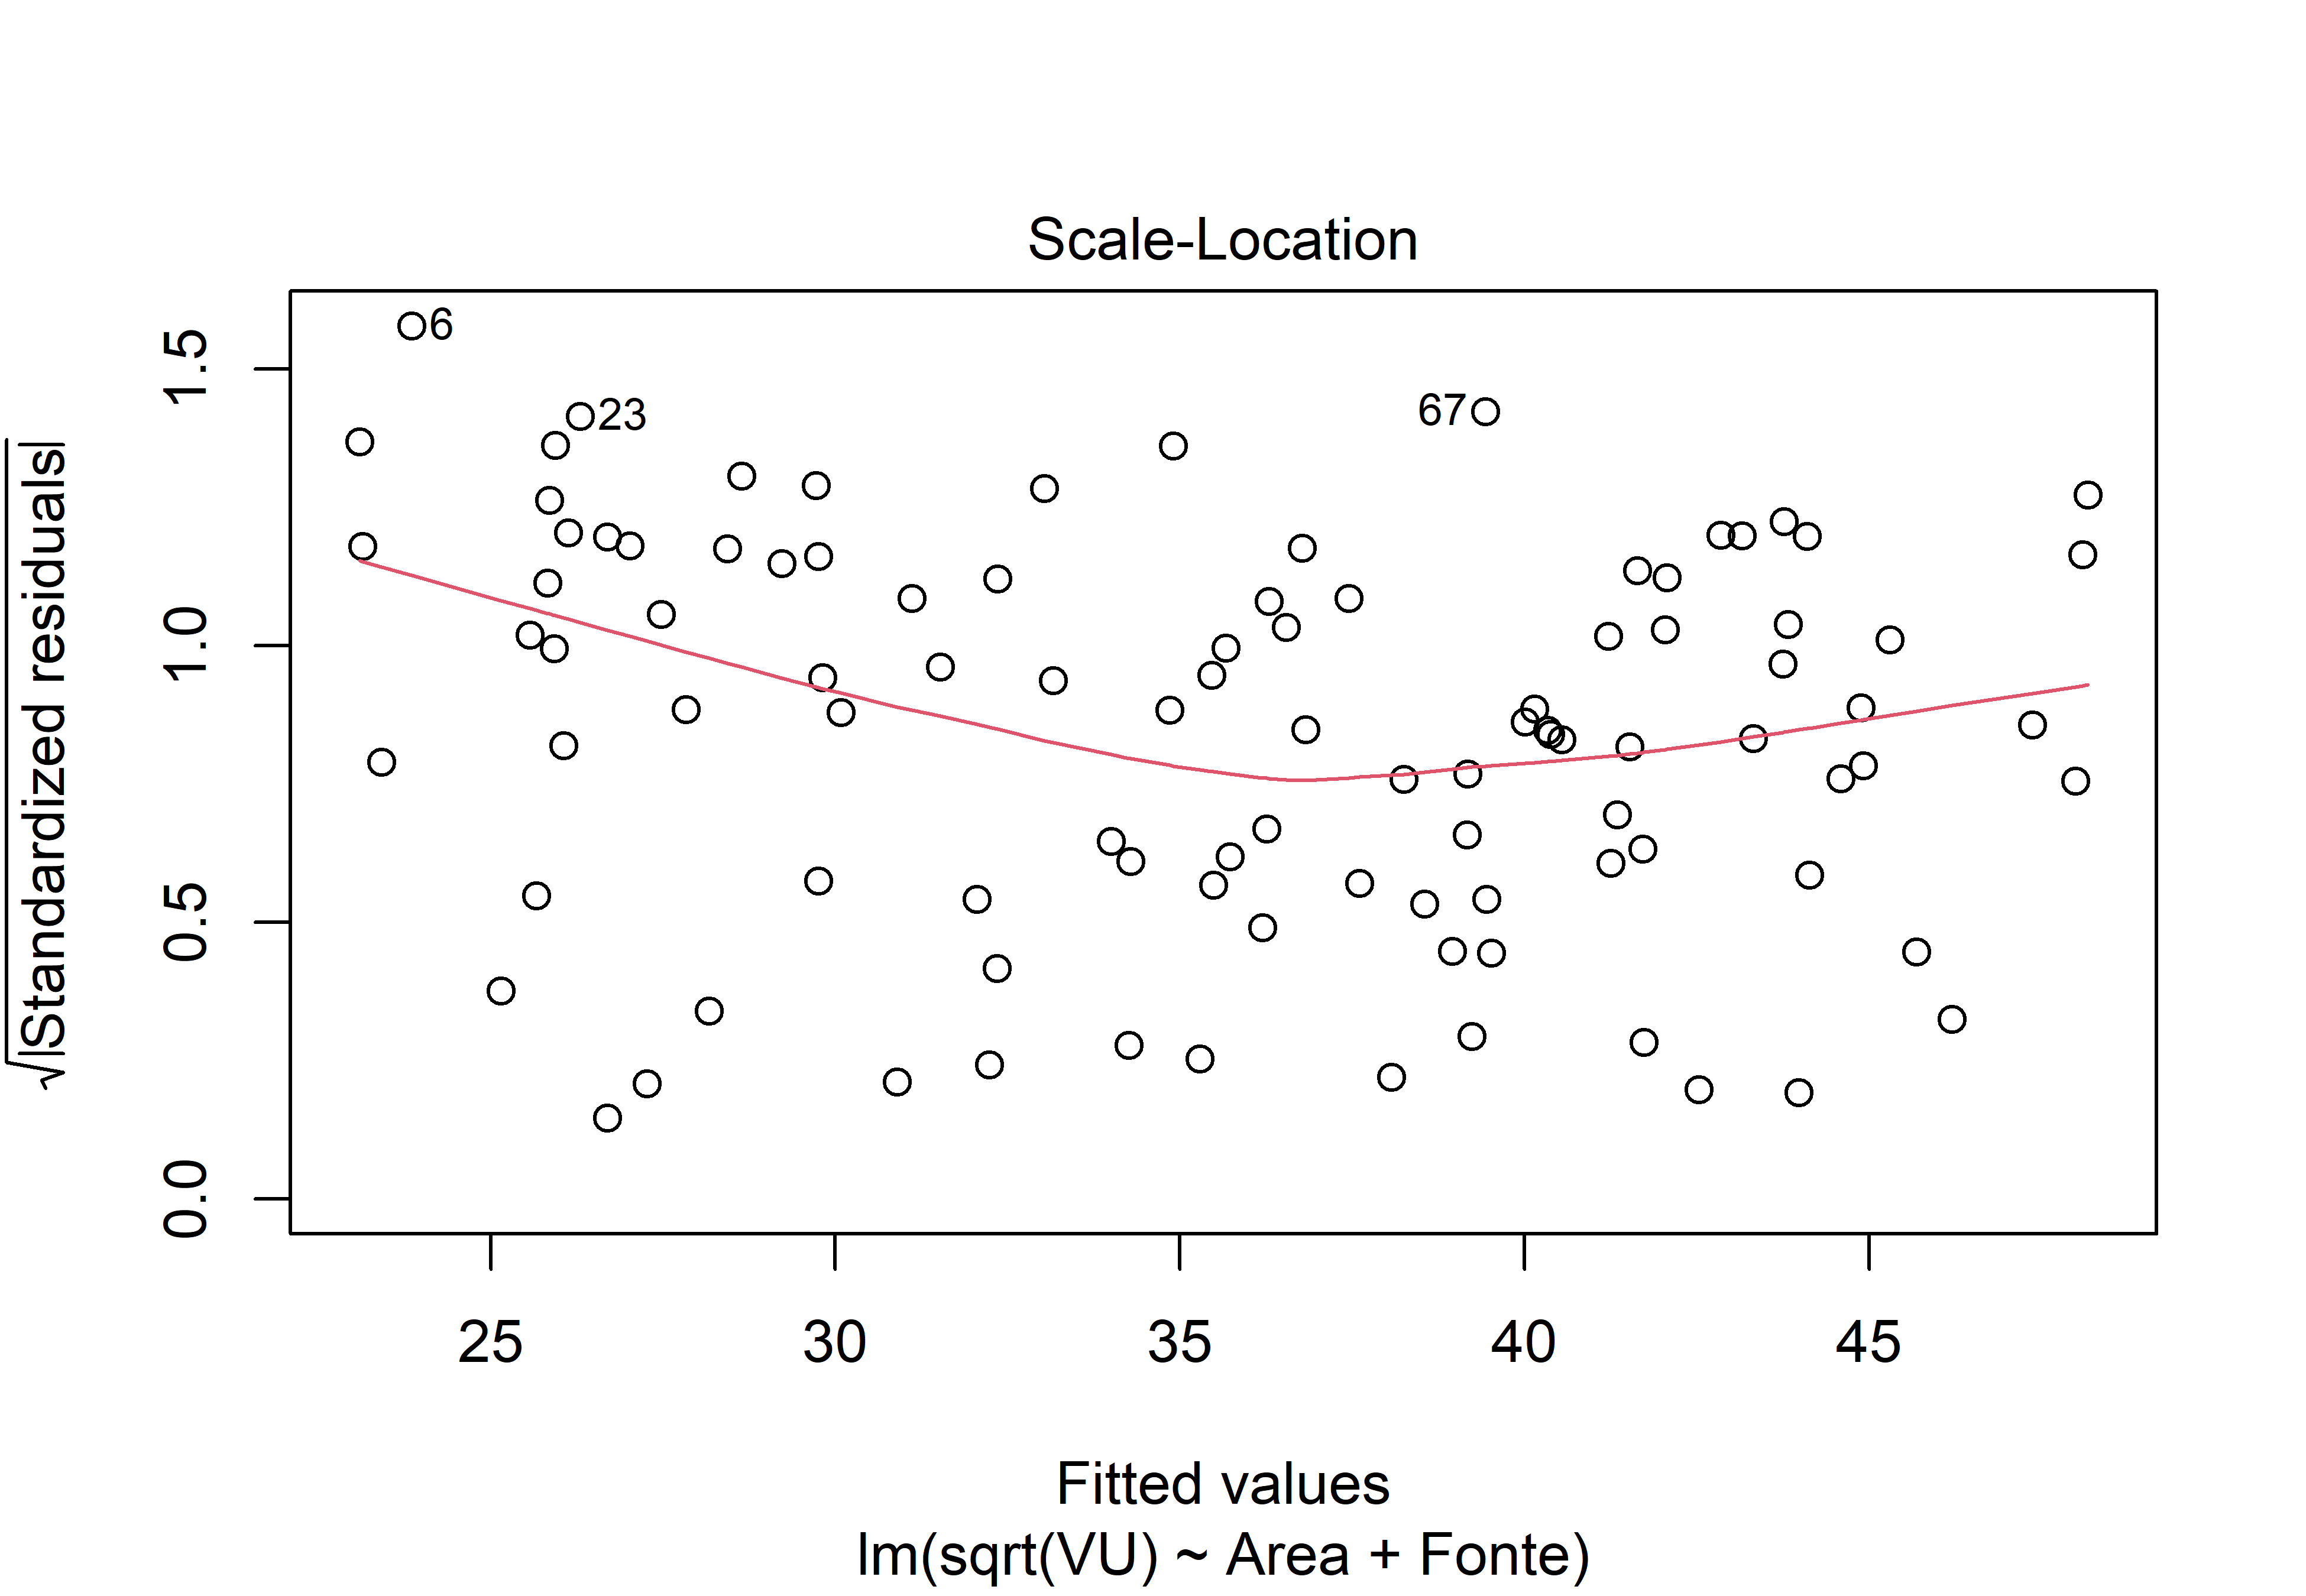
\includegraphics[width=0.5\linewidth]{./images/fit3Diagnostics-3} 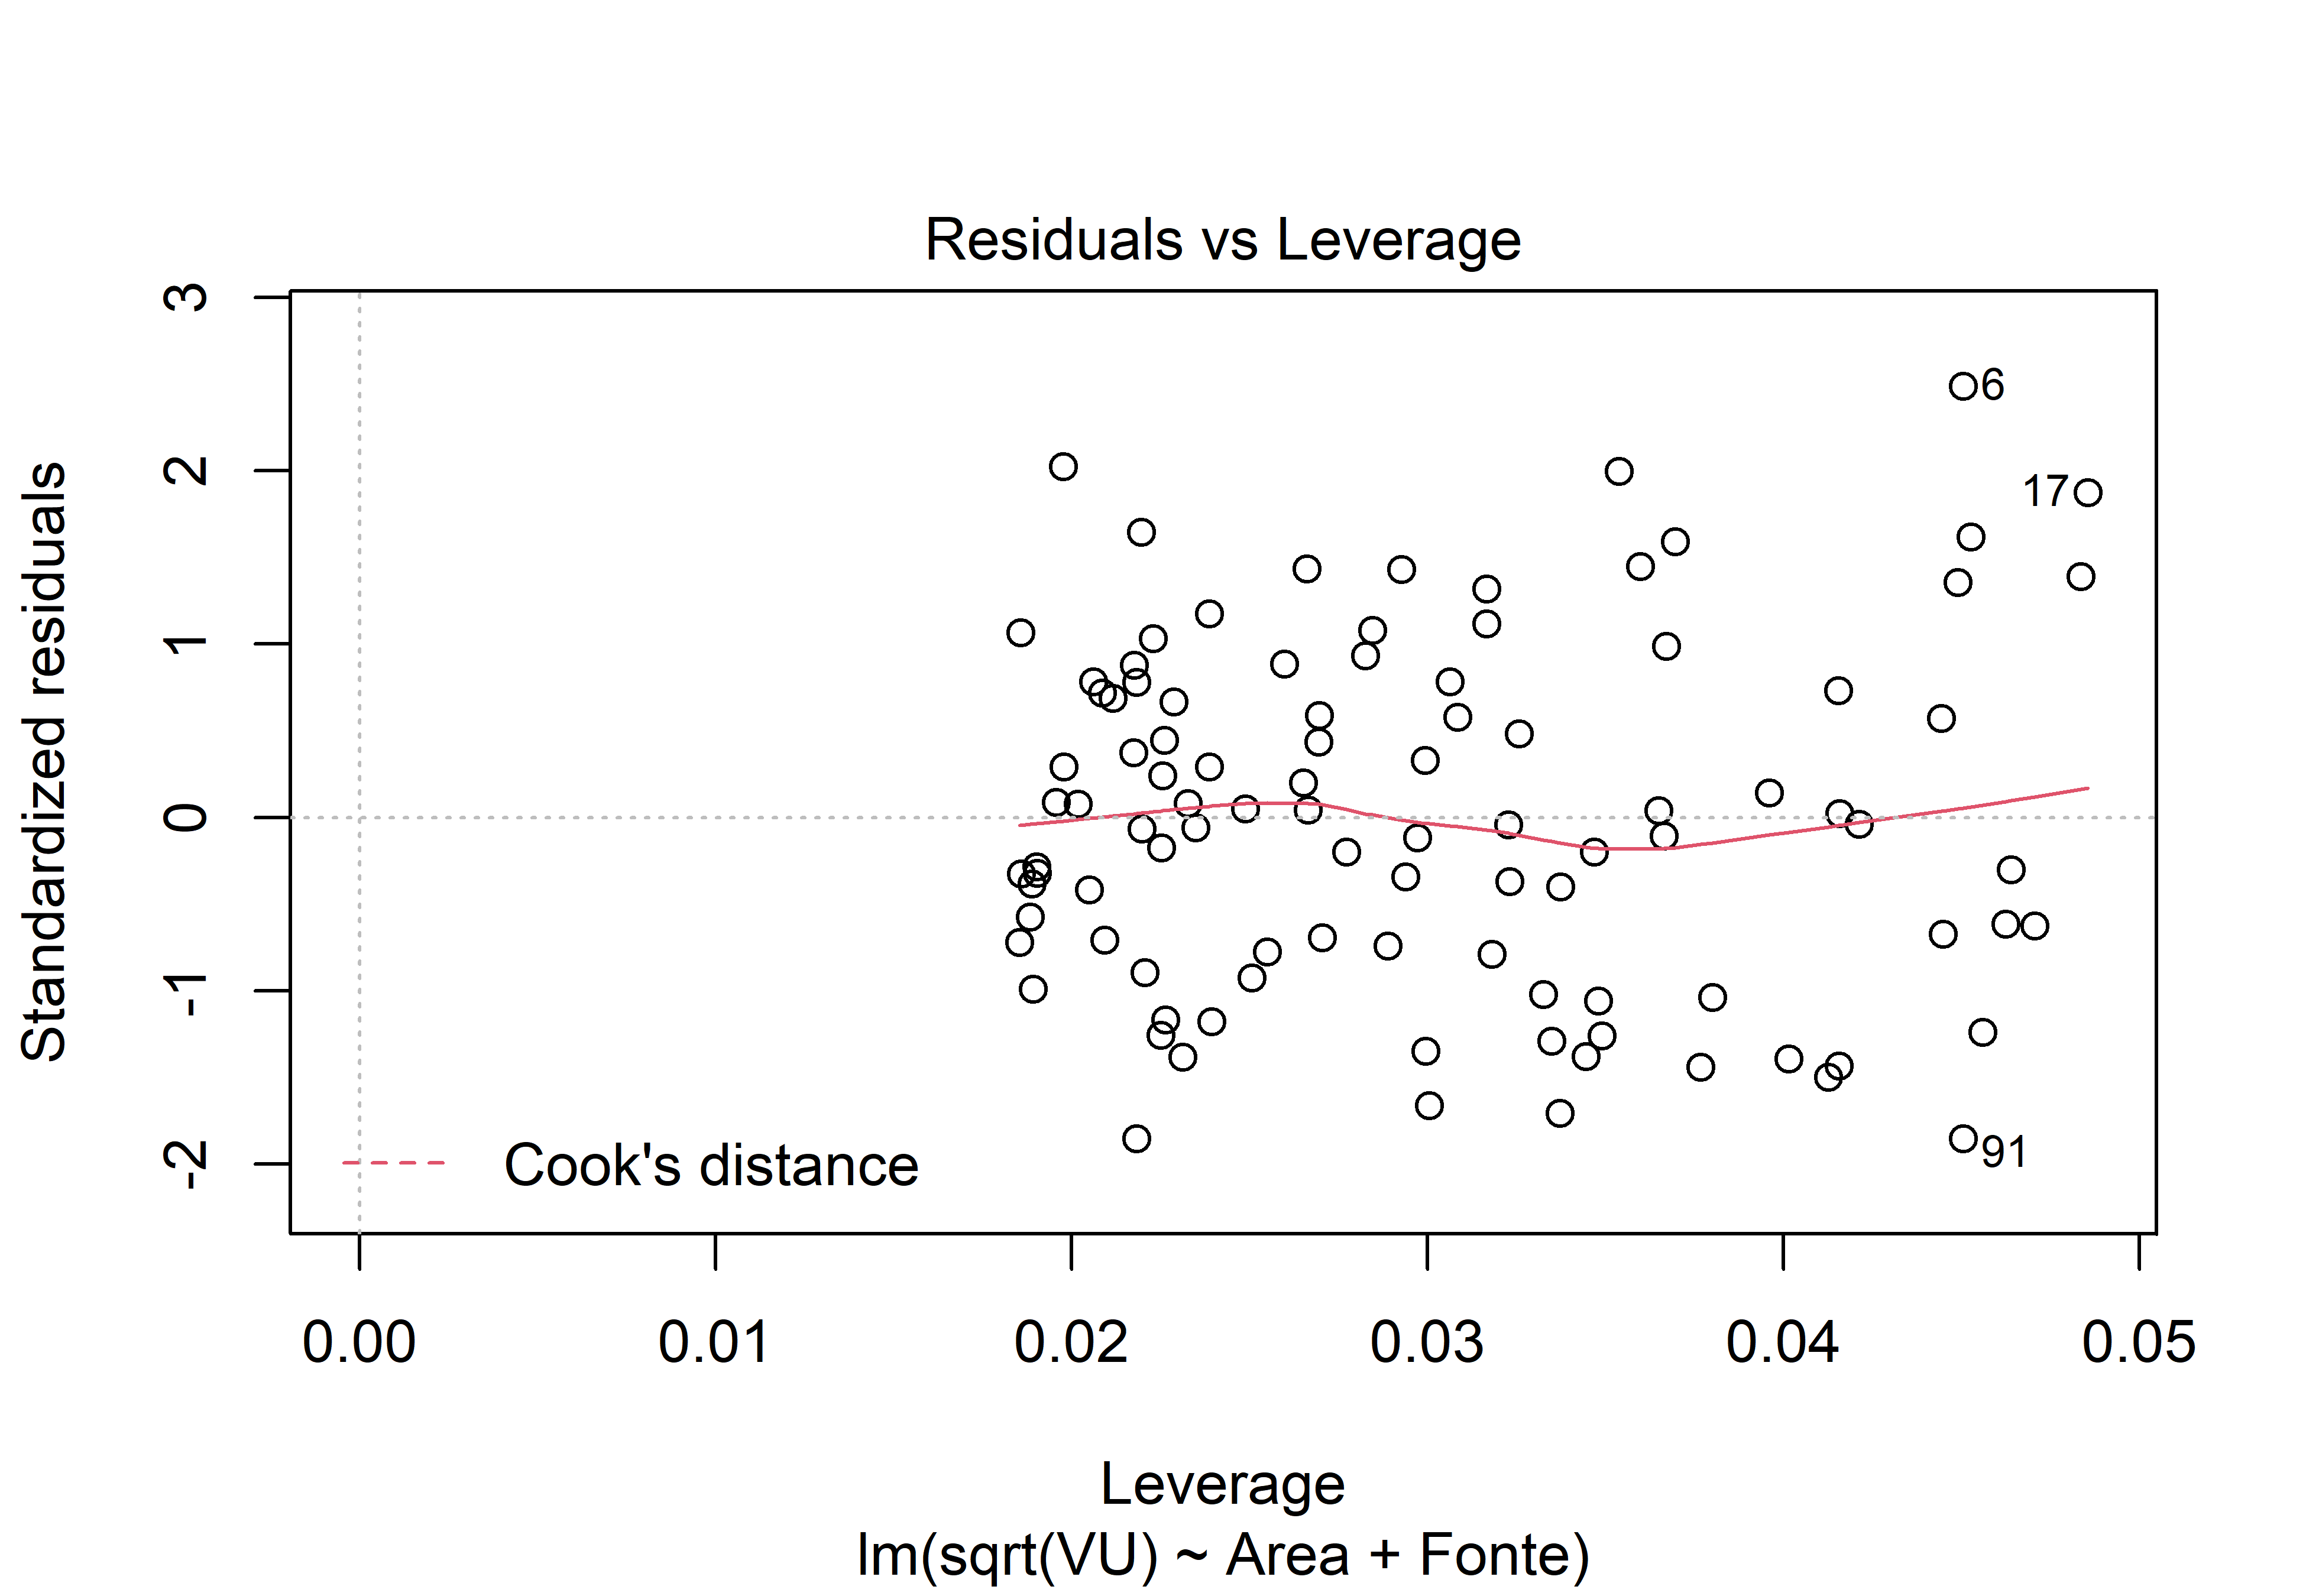
\includegraphics[width=0.5\linewidth]{./images/fit3Diagnostics-4} \caption{Modelo mau especificado. Fator oferta.}\label{fig:fit3Diagnostics}
\end{figure}

\begin{figure}
\centering
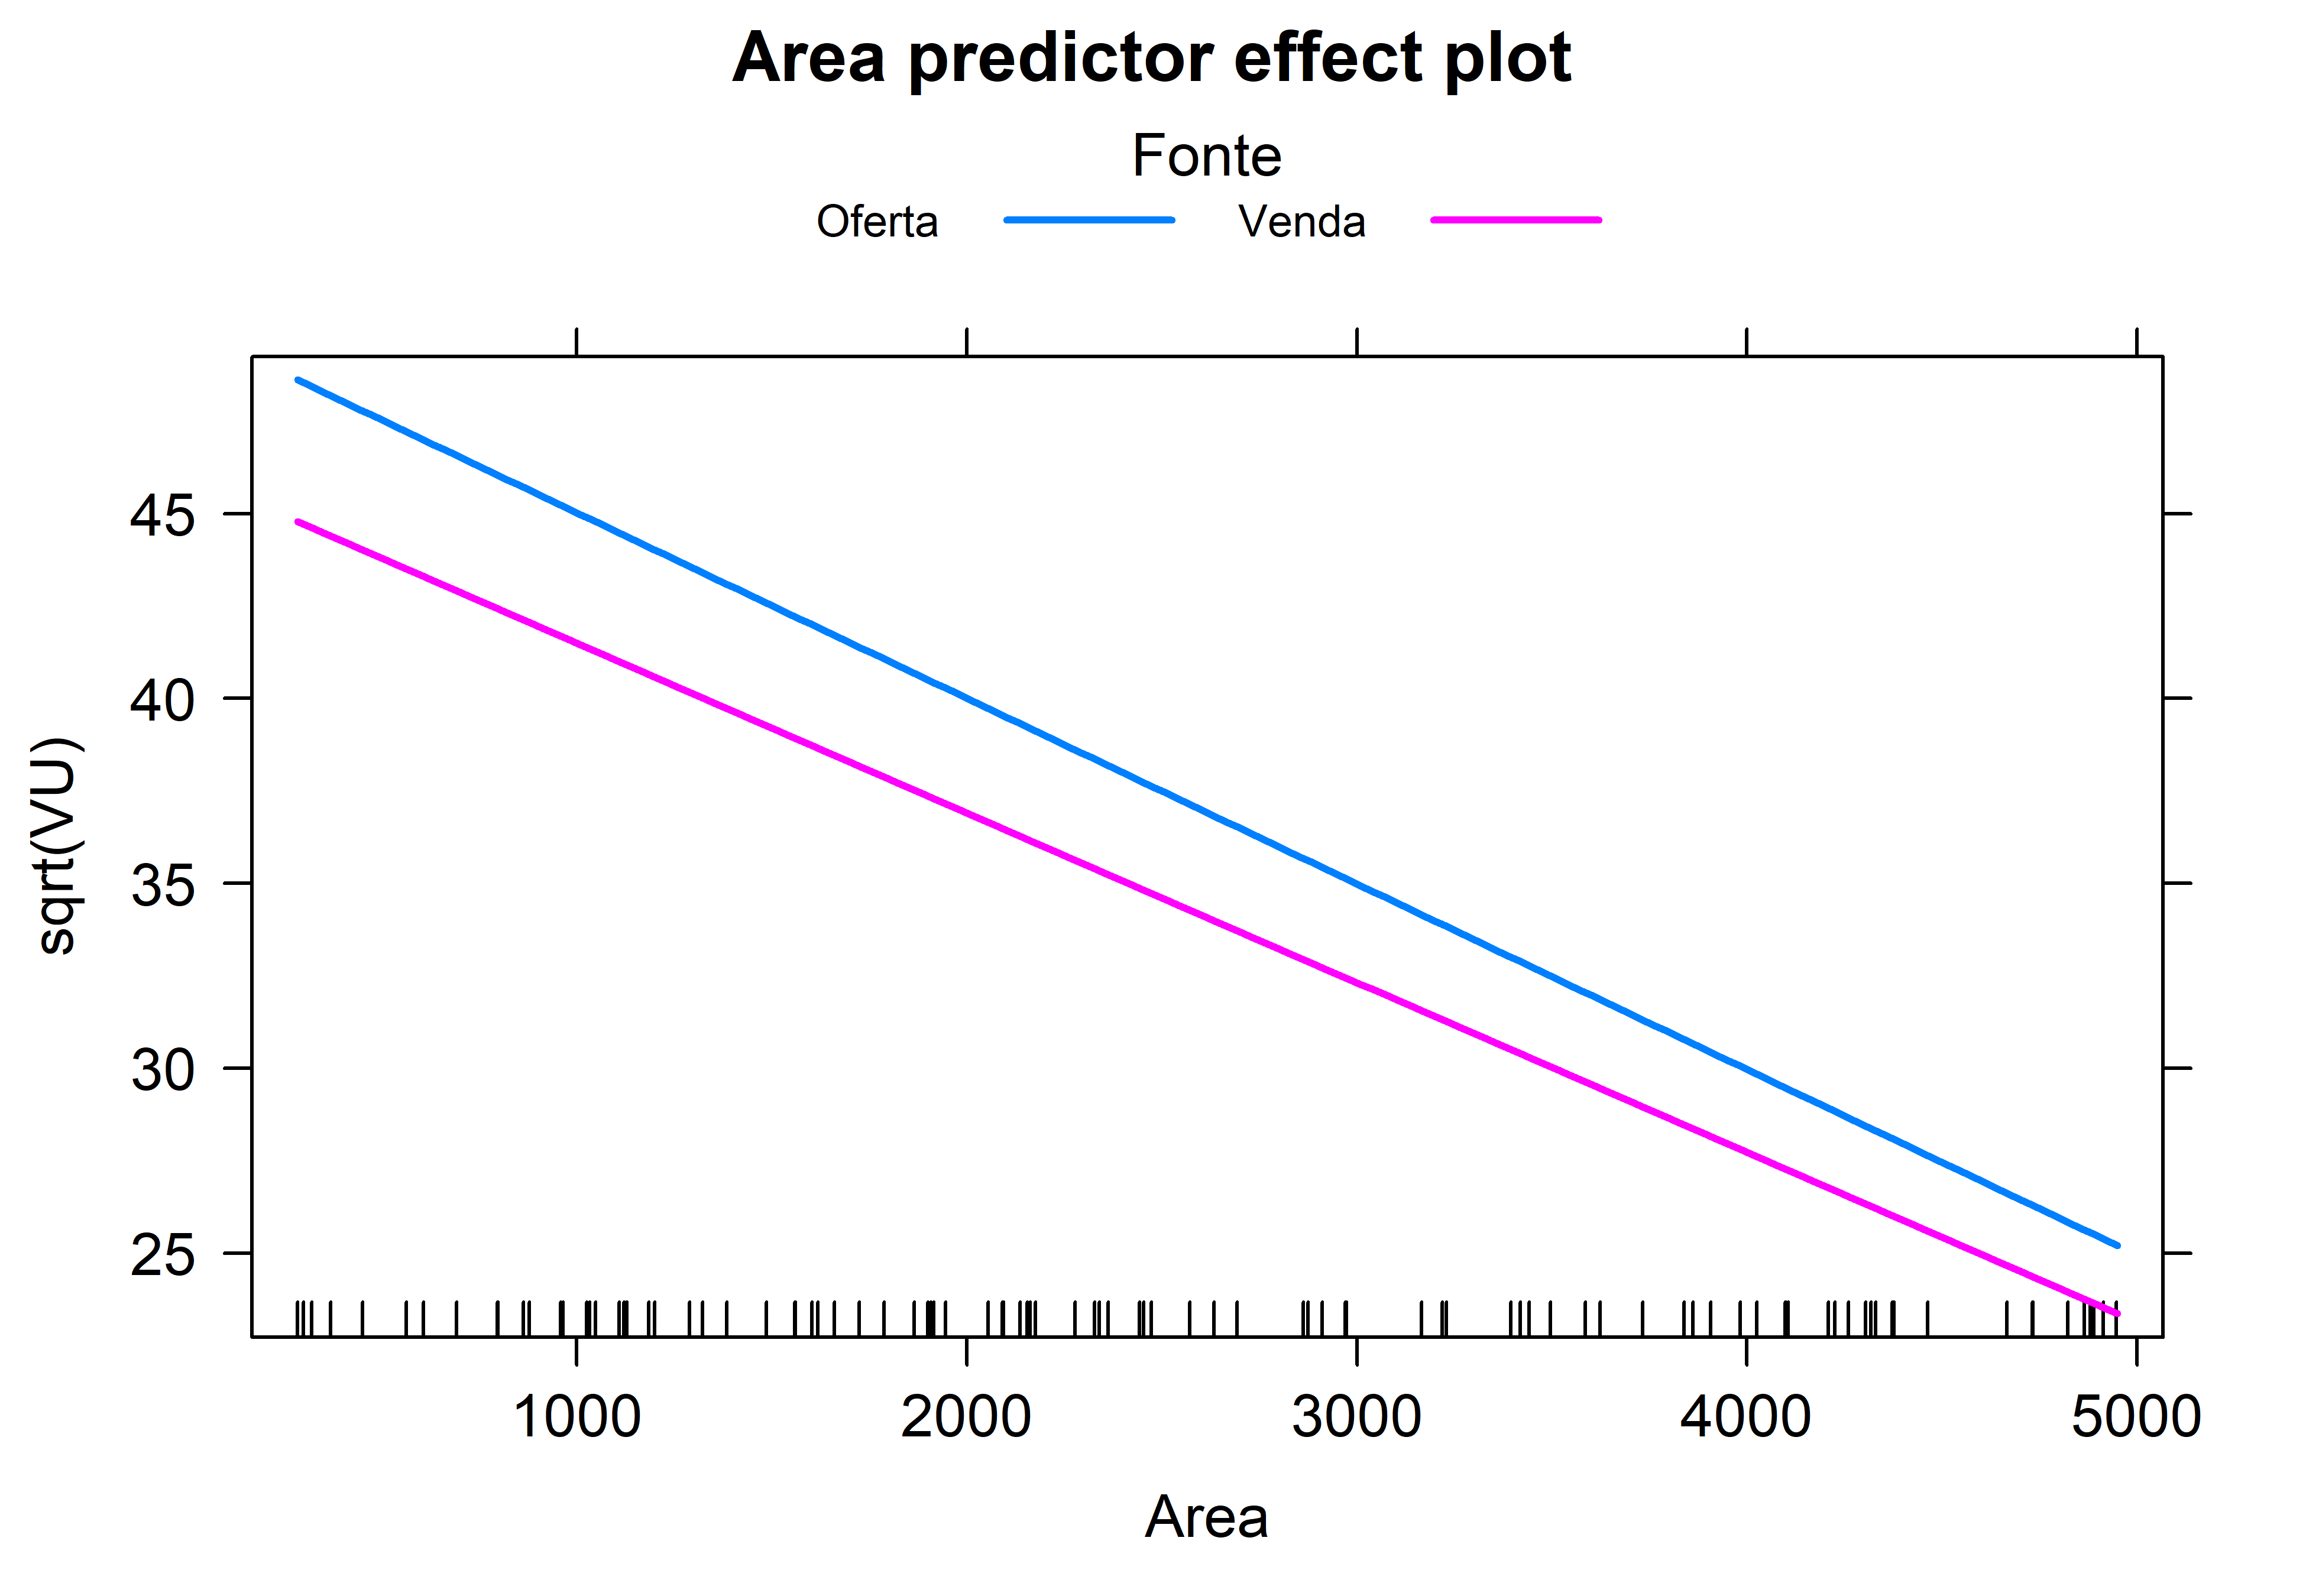
\includegraphics{./images/rightModel3-1.png}
\caption{Fator oferta com transformação raiz quadrada. Modelo
especificado corretamente.}
\end{figure}

\begin{verbatim}
## `geom_smooth()` using method = 'loess' and formula 'y ~ x'
\end{verbatim}

\begin{verbatim}
## `geom_smooth()` using formula 'y ~ x'
\end{verbatim}

\begin{verbatim}
## `geom_smooth()` using method = 'loess' and formula 'y ~ x'
\end{verbatim}

\begin{figure}
\centering
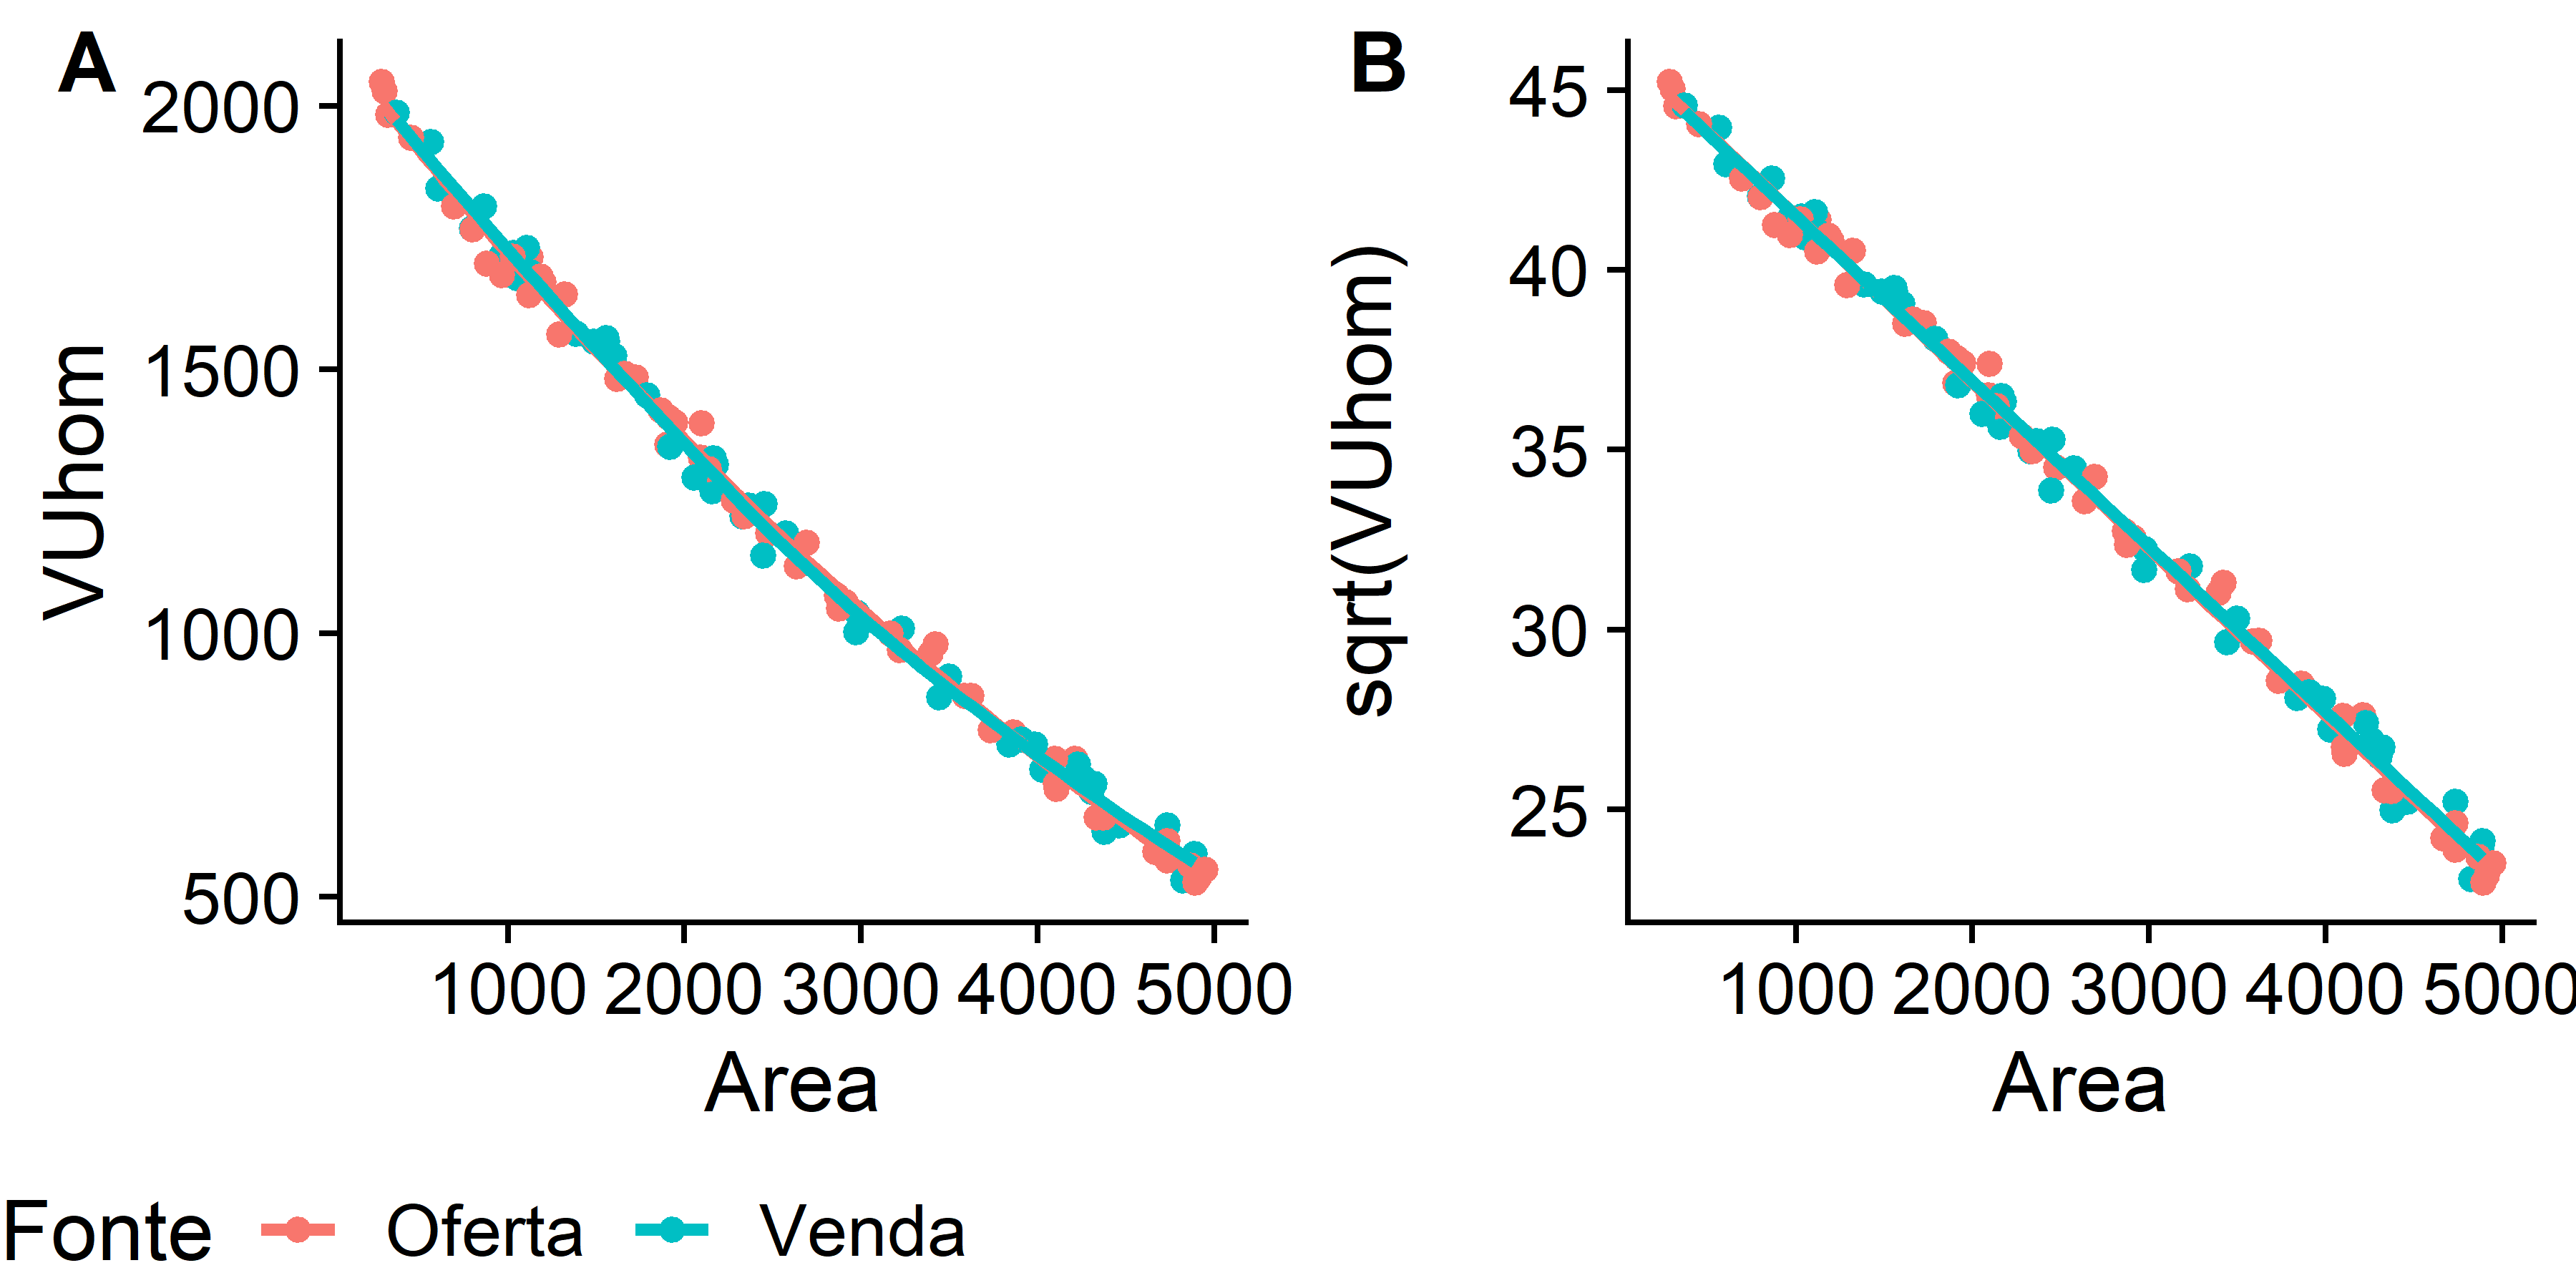
\includegraphics{./images/dadosHomogeneizados3-1.png}
\caption{Dados homogeneizados. Transformação raiz quadrada.}
\end{figure}

\hypertarget{conclusuxe3o}{%
\section{Conclusão}\label{conclusuxe3o}}

Quando da utilização de dados de oferta para elaboração de modelos, além
do valor da estimativa central, também os limites do intervalo de
confiança devem ser ajustados pelo fator oferta.

Pelo procedimento preconizado na atual normativa, o intervalo de
confiança é simplesmente transladado. Isso implica que o valor inferior
do intervalo de confiança acaba minorado por um fator superior ao fator
oferta, enquanto o limite superior do intervalo de confiança é minorado
com um fator menor do que o fator oferta.

Quando a amplitude do intervalo de confiança é relativamente pequena,
como no estudo de caso apresentado, esta diferença tende também a ser
pequena, podendo até, em alguns casos, ser negligenciável.

No entanto, caso a amplitude do intervalo de confiança seja
relativamente grande, isto passa a ser um problema, pois os intervalos
de valores admissíveis calculados conforme preconiza a NBR 14.653-02,
tendem a tornar-se fortemente assimétricos, como ilustrado pelo segundo
caso apresentado, com dados simulados, já que o limite do campo de
arbítrio inferior é atingido.

\hypertarget{referuxeancias}{%
\section*{Referências}\label{referuxeancias}}
\addcontentsline{toc}{section}{Referências}

\hypertarget{refs}{}
\leavevmode\hypertarget{ref-NBR1465302}{}%
ABNT. 2011. \emph{NBR 14653-2: Avaliação de Bens -- Parte 2: Imóveis
Urbanos}. Rio de Janeiro: Associação Brasileira de Normas Técnicas.

\leavevmode\hypertarget{ref-chinloy}{}%
Chinloy, Peter T. 1980. ``An Empirical Model of the Market for Resale
Homes.'' \emph{Journal of Urban Economics} 7 (3): 279--92.
\url{https://doi.org/https://doi.org/10.1016/0094-1190(80)90001-7}.

\leavevmode\hypertarget{ref-faraway2004linear}{}%
Faraway, J. J. 2004. \emph{Linear Models with R}. Chapman \& Hall/Crc
Texts in Statistical Science. Taylor \& Francis.
\url{https://books.google.com.br/books?id=fvenzpofkagC}.

\leavevmode\hypertarget{ref-haurin}{}%
Haurin, Donald, Stanley McGreal, Alastair Adair, Louise Brown, and James
R. Webb. 2013. ``List Price and Sales Prices of Residential Properties
During Booms and Busts.'' \emph{Journal of Housing Economics} 22 (1):
1--10. \url{https://doi.org/https://doi.org/10.1016/j.jhe.2013.01.003}.

\leavevmode\hypertarget{ref-horowitz}{}%
Horowitz, Joel L. 1992. ``The Role of the List Price in Housing Markets:
Theory and an Econometric Model.'' \emph{Journal of Applied
Econometrics} 7 (2): 115--29. \url{http://www.jstor.org/stable/2285023}.

\leavevmode\hypertarget{ref-matloff2009}{}%
Matloff, Norman Saul. 2009. \emph{From Algorithms to Z-Scores:
Probabilistic and Statistical Modeling in Computer Science}. Davis,
California: Orange Grove Books.
\url{http://heather.cs.ucdavis.edu/~matloff/132/PLN/probstatbook/ProbStatBook.pdf}.

\leavevmode\hypertarget{ref-mooya2009}{}%
Mooya, Manya M. 2009. ``Market Value Without a Market: Perspectives from
Transaction Cost Theory.'' \emph{Urban Studies} 46 (3): 687--701.
\url{http://www.jstor.org/stable/43197982}.

\bibliographystyle{unsrt}
\bibliography{references.bib}


\end{document}
